\documentclass[titlepage,12pt,twoside]{article}
%\usepackage[a4paper, inner=25mm, outer=20mm, top=20mm, bottom=20mm, bindingoffset=0mm]{geometry}

\raggedbottom
\pagenumbering{arabic}
\textheight=240mm
\textwidth=150mm
\parskip=0pt plus3pt
\marginparwidth=22mm
\marginparsep=3mm

\setcounter{secnumdepth}{5}
\setcounter{tocdepth}{4}

\usepackage{filecontents}
\usepackage{graphicx}
\graphicspath{{/Users/laci/Schule/Diplomarbeit_GitHub/LATEX_DOKU_DA/src}}
\usepackage{tabularx}
\usepackage{multirow}
\usepackage{xcolor}
\usepackage{caption}
\usepackage[autostyle]{csquotes}
\usepackage{circuitikz}
\usepackage{amsmath}
\usepackage{textgreek}
\usepackage{siunitx}
\usepackage[utf8]{inputenc}
\usepackage[ngerman]{babel}
\usepackage[margin=2.2cm]{geometry}
\usepackage[none]{hyphenat}
\usepackage{float} % für Positionierungsoption [H] beie Tables, figures,...
\usepackage{hyperref} %Für URLS
\usepackage{listings} %Für Codezeilen
\usepackage{titlesec} %Für Buchstaben als Überschriftsnummerierung
\usepackage{enumitem}
\usepackage{pdfpages} %Für A3-Seiten
\usepackage{siunitx}
\lstset{language=C++}
\setlength{\fboxsep}{5pt} % Ändere die Rahmenbreite nach Bedarf
%--------------------------------------------------------------------------
%--------------------------------------------------------------------------
\usepackage{fancyhdr}
\pagestyle{fancy}
\fancyhf{}
\setlength{\headheight}{20pt}
\fancyhead[LE,RO]{\rightmark}

\fancyfoot[L]{\small{Al-Maytah, Schweitzer, Szabo}}
\fancyfoot[C]{}
\fancyfoot[R]{\arabic{page}}

\usepackage[round, sort, authoryear]{natbib}
%\usepackage[nottoc]{tocbibind}
%--------------------------------------------------------------------------
%--------------------------------------------------------------------------
%==DOKUMENTBEGINN==========================================================

\begin{document}

\pagenumbering{gobble}

%--------------------------------------------------------------------------
%--------------------------------------------------------------------------
%==TITELSEITE==============================================================

\begin{titlepage}

	\begin{center}
	\begin{tabular}{p {2.4cm} p{10.8cm} p{2cm}}
	
\includegraphics[width=0.16\textwidth,page=1]{/Users/laci/Schule/Diplomarbeit_GitHub/LATEX_DOKU_DA/src/TGM_logo.pdf}& \large{{\textbf{HTBLVA Technologisches Gewerbemuseum}}}\par\par\centering{\scriptsize{\textbf{Höhere Lehranstalt für Elektronik und Technische Informatik}}}&
\includegraphics[width=0.12\textwidth,page=1]{/Users/laci/Schule/Diplomarbeit_GitHub/LATEX_DOKU_DA/src/HTL.png}\\
	\end{tabular}
	\noindent\rule{1.1\textwidth}{1pt} 
	\end{center}
	
	\begin{center}
	
	\vspace*{1cm}
	\LARGE
	\textbf{DIPLOMARBEIT}
	
	\vspace{1.7cm}
	\normalsize
	Gesamtprojekt\\
	\LARGE
	\textbf{RoboGlove - Bionische Hand}\\
	\end{center}
	
	\vspace{1.7cm}
	
	\normalsize 
	\large
	
	\begin{center}
		\begin{tabular}{llr} 
			\multicolumn{3}{c}{\large{\textbf{3D-Druck, Mechanik, User-Interface Programmierung}}} \\
			\large{Amir Al-Maytah} & \hspace{0.3cm}\large{5BHEL}\hspace{0.3cm} &  \large{Betreuer: Prof. Dipl.-Ing. Christoph Diemberger}\\
			\\
			\multicolumn{3}{c}{\large{\textbf{Mikrokontroller-Programmierung, Testmanagement, Gesamtintegration}}} \\
			\large{Fabian Schweitzer} & \hspace{0.3cm}\large{5BHEL}\hspace{0.3cm} &  \large{Betreuer: Prof. Dipl.-Ing. Christoph Diemberger}\\
			\\
			\multicolumn{3}{c}{\large{\textbf{Hardwareentwicklung, PCB-Design, Projektleitung}}} \\
			\large{Ladislaus Szabo} & \hspace{0.3cm}\large{5BHEL}\hspace{0.3cm} &  \large{Betreuer: Prof. Dipl.-Ing. Christoph Diemberger}\\
			\\
		\end{tabular}
	\end{center}
	
	
	
	\vspace{1.5cm}
	\normalsize
	Ausgeführt im Schuljahr 2023/2024\\
	\vspace{0.7cm}
	\noindent\rule{\textwidth}{1pt}
	\begin{tabular}{lr}
	Abgabevermerk:\\
	\\
	\\
	Datum: 13.2.2024 &\hspace{4cm}   übernommen von:\\
	\end{tabular}
	
	\end{titlepage}
	
	\newpage
	\thispagestyle{empty}
	\clearpage\mbox{}\clearpage

%--------------------------------------------------------------------------
%--------------------------------------------------------------------------
%==EIDESSTATTLICHE-ERKLÄRUNG===============================================

\thispagestyle{empty}
	
\begin {center}
	\begin{tabular} {p{3cm} p{1cm} p{1cm}}
  & 
  & 
  \vspace{1mm}\centering{
\includegraphics[width=0.2\textwidth,page=1]{/Users/laci/Schule/Diplomarbeit_GitHub/LATEX_DOKU_DA/src/TGM_logo.pdf}}\\ 
\end{tabular}

\hspace{40mm}

\color{white}

\color{blue}	
\Large{\bfseries{Eidesstattliche Erklärung}}	
\color{black}	

\end {center}

\hspace{10mm}

Hiermit versichere ich, dass ich die vorliegende Arbeit selbstständig verfasst und keine anderen Hilfsmittel als die angegebenen benützt habe. Die Stellen, die anderen Werken (gilt ebenso für Werke
aus elektronischen Datenbanken oder aus dem Internet) wörtlich oder sinngemäß entnommen sind, habe ich unter Angabe der Quelle und Einhaltung der Regeln wissenschaftlichen Zitierens kenntlich
gemacht. Diese Versicherung umfasst auch in der Arbeit verwendete bildliche Darstellungen, Tabellen, Skizzen und Zeichnungen. Für die Erstellung der Arbeit habe ich auch folgende Hilfsmittel generativer
KI-Tools (z. B. ChatGPT, Grammarly Go, Midjourney) zu folgendem Zweck verwendet: [Bitte hier Einsatzgebiet anführen.]. Die verwendeten Hilfsmittel wurden vollständig und wahrheitsgetreu inkl. Produktversion 
und Prompt ausgewiesen. \\

\begin{tabular}{p{7cm}}
\\
\vspace{3cm}
------------------------------------------------\\
Amir Al-Maytah\\
\vspace{3cm}
------------------------------------------------\\
Fabian Schweitzer\\
\vspace{3cm}
------------------------------------------------\\
Ladislaus Szabo\\


\end{tabular}

\newpage
\thispagestyle{empty}
\clearpage\mbox{}\clearpage

%--------------------------------------------------------------------------
%--------------------------------------------------------------------------
%==DANKSAGUNG==============================================================

\thispagestyle{empty}

\begin{center}
\Large{\textbf{Danksagung}} 
\end{center}

\hspace{2cm}
\\
Wir möchten uns herzlich bei unserem Betreuer Dipl.-Ing. Christoph Diemberger bedanken, 
der uns bei diesem Projekt grundlegend unterstützt und motiviert hat. \\
\\
Des Weiteren gilt unser Dank auch Fachlehrer Robert Offner und allen anderen Lehrpersonen, 
die uns in der Werkstatt betreut und geholfen haben. \\
\\
Wir danken allen, die uns im Rahmen dieses Projekts zur Seite standen.      

\newpage
\thispagestyle{empty}
\clearpage\mbox{}\clearpage

%--------------------------------------------------------------------------
%==========================================================================
%== Diploma Thesis Englisch ===============================================

\thispagestyle{empty}
	
\begin {center}
\begin{tabular} {|p {3cm}|p{8cm}|p{4.55cm}|}
 \hline 
\vspace{1mm}
 \centering{
\includegraphics[width=0.20\textwidth,page=1]{/Users/laci/Schule/Diplomarbeit_GitHub/LATEX_DOKU_DA/src/TGM_logo.pdf}} &
\centering{\normalsize{\textbf{HTBLVA Wien 20}}\par\small{\textbf{College of}\par Electronic and Technical Information Technology}} &
	\small{\bfseries{Diploma\par Exam}}\\ 
	\hline
\end{tabular}

\vspace{5mm}
\Large{\textbf{DIPLOMA THESIS\\}}
\vspace{1mm}
\small{\textbf{DOCUMENTATION\\}}
\vspace{5mm}  

	\begin{tabular} {|p {6cm}|p{10cm}|}
	 \hline 
		\bfseries{\small{Authors}} & \small{Amir Al-Maytah, Fabian Schweitzer, Ladislaus Szabo}\\
	 \hline
	  \bfseries{\small{From\par Academic year}} & \small{5BHEL 2023/2024}\\
	 \hline 
	  \bfseries{\small{Topic}} & \small{RoboGlove - Bionische Hand}\\ 
	 \hline 
	  \bfseries{\small{CO-operation partners}} & \small{}\\ 
	 \hline
	\multicolumn{2}{l}{\large{ \textbf{}}}\\
	 \hline
	  \bfseries{\small{Assignment of tasks}} & \small{As part of a feasibility study, a robotic hand is to be controlled by means of a glove. For
	  this purpose, various sensors must be tested for accuracy and the evaluated data then
	  transmitted wirelessly to the robotic hand. The positions of the fingers are to be displayed in a
	  user interface.}\\
	 \hline
	\multicolumn{2}{l}{\large{ \textbf{}}}\\ 
	 \hline
	  \bfseries{\small{Realization}} & \small{The movements of the human hand are recorded with Flex sensors on the glove.
	  The required data is then transmitted to the robotic hand via Bluetooth. A website will serve as
	  the user interface.}\\  
	 \hline
	\multicolumn{2}{l}{\large{ \textbf{}}}\\ 
	 \hline
	  \bfseries{\small{Results}} & \small{The hand movements can be correctly evaluated and transmitted. The user wears the
	  glove and grasps an object. The servo motors interpret the received data by means of the PCB
	  and enable the robot hand to also grasp the same object. When the hand is opened, the robot
	  hand must also move back to its starting position.}\\
	 \hline
	\end{tabular}
\end {center}

\thispagestyle{empty}
	
\newpage
\thispagestyle{empty}

\begin{centering}
\begin{tabular} {|p {3cm}|p{8cm}|p{4.55cm}|}
 \hline 
\vspace{1mm}
 \centering{
\includegraphics[width=0.20\textwidth,page=1]{/Users/laci/Schule/Diplomarbeit_GitHub/LATEX_DOKU_DA/src/TGM_logo.pdf}} &
\centering{\normalsize{\textbf{HTBLVA Wien 20}}\par\small{\textbf{College of}\par Electronic and Technical Information Technology}} &
	\small{\bfseries{Diploma\par Exam}}\\ 
	\hline
\end{tabular}

\vspace {2mm}

	\begin{tabular} {|p {6cm}|p{10cm}|}
	 \hline 
		\bfseries{\small{Illustrative graph, photo\par (with explanation)}} & \vspace{0.0mm} \small{
		
\includegraphics[width=0.666\textwidth]{/Users/laci/Schule/Diplomarbeit_GitHub/LATEX_DOKU_DA/src/TGM_logo.pdf} \par Final construction of the System
		}\\
	 \hline
	  \multicolumn{2}{l}{\large{ \textbf{}}}\\
	 \hline
	  \bfseries{\small{Participation in competitions,\par Awards}} & \small{}\\
	 \hline 
	  \multicolumn{2}{l}{\large{ \textbf{}}}\\
	 \hline
	  \bfseries{\small{Accesibility
		of\par Diploma Thesis}} & \small{Department administration}\\ 
	 \hline 
	  \multicolumn{2}{l}{\large{ \textbf{}}}\\
	\end{tabular}  
	
	\begin{tabular} {|p {6cm}|p{5cm}|p{4.6cm}|}
	 \hline
   \vspace{5mm}
	  \bfseries{\small{Approval\par (Date/Signature)}} \vspace{5mm} & \tiny{Examiner} & \tiny{Head of College/Department}\\ 
	 \hline 
	\end{tabular} 
	\end{centering}

\thispagestyle{empty}

\newpage

%--------------------------------------------------------------------------
%==========================================================================
%== Diploma Thesis Deutsch ================================================

\thispagestyle{empty}
	
\begin {center}
\begin{tabular} {|p {3cm}|p{8cm}|p{4.55cm}|}
 \hline 
\vspace{1mm}
 \centering{
\includegraphics[width=0.20\textwidth,page=1]{/Users/laci/Schule/Diplomarbeit_GitHub/LATEX_DOKU_DA/src/TGM_logo.pdf}} &
\centering{\normalsize{\textbf{HTBLVA Wien 20}}\par\small{\textbf{Höhere Technische Lehranstalt für}\par Elektronik und Technische  Informatik}} &
	\small{\bfseries{Reife- und\par Diplomprüfung}}\\ 
	\hline
\end{tabular}

\vspace{5mm}
\Large{\textbf{DIPLOMARBEIT\\}}
\vspace{1mm}
\small{\textbf{DOKUMENTATION\\}}
\vspace{5mm}  

	\begin{tabular} {|p {6cm}|p{10cm}|}
	 \hline 
		\bfseries{\small{Namen der\par Verfasser/innen}} & \small{Amir Al-Maytah, Fabian Schweitzer, Ladislaus Szabo}\\
	 \hline
	  \bfseries{\small{Jahrgang\par Schuljahr}} & \small{5BHEL 2023/2024}\\
	 \hline 
	  \bfseries{\small{Thema der Diplomarbeit}} & \small{RoboGlove - Bionische Hand}\\ 
	 \hline 
	  \bfseries{\small{Kooperationspartner}} & \small{}\\ 
	 \hline
	\multicolumn{2}{l}{\large{ \textbf{}}}\\
	 \hline
	  \bfseries{\small{Aufgabenstellung}} & \small{Im Rahmen eines Diplomprojekts soll eine Roboterhand mittels eines Handschuhs gesteuert werden. 
	  Dazu müssen verschiedene Sensoren auf Genauigkeit getestet und aanscließend die ausgewerteten Daten kabellos an die
	  Roboterhand übertragen werden. Die Bewegungen der Finger sollen mit Motoren nachgebildet werden und die Stellungen
	  dieser soll im User-Interface dargestellt werden.}\\
	 \hline
	\multicolumn{2}{l}{\large{ \textbf{}}}\\ 
	 \hline
	  \bfseries{\small{Realisierung}} & \small{Die Bewegungen der menschlichen Hand werden mit Flexsensoren am Handschuh erfasst. Die benötigten Daten werden
	  anschließend über ein drahtloses Protokoll an die Roboterhand übertragen. Die Bewegungen der Roboterfinger werden mit
	  Servomotoren realisiert. Als User-Interface soll eine Application dienen.}\\  
	 \hline
	\multicolumn{2}{l}{\large{ \textbf{}}}\\ 
	 \hline
	  \bfseries{\small{Ergebnisse}} & \small{Die Handbewegungen können korrekt ausgewertet und übertragen werden. Der Benutzer trägt den Handschuh und greift 
	  ein Objekt. Die Servomotoren interpretieren mittels des PCBs die empfangenen Daten und ermöglichen es der Roboterhand 
	  ebenfalls das gleiche Objekt zu greifen. Beim Öffnen der Hand muss sich die Roboterhand in ihre Ausgangsstellung 
	  zurückbewegen.}\\
	 \hline
	\end{tabular}
\end {center}
\thispagestyle{empty}
	
\newpage
\thispagestyle{empty}

\begin{centering}
\begin{tabular} {|p {3cm}|p{8cm}|p{4.55cm}|}
 \hline 
\vspace{1mm}
 \centering{
\includegraphics[width=0.20\textwidth,page=1]{/Users/laci/Schule/Diplomarbeit_GitHub/LATEX_DOKU_DA/src/TGM_logo.pdf}} &
\centering{\normalsize{\textbf{HTBLVA Wien 20}}\par\small{\textbf{Höhere Technische Lehranstalt für}\par Elektronik und Technische  Informatik}} &
	\small{\bfseries{Reife- und\par Diplomprüfung}}\\ 
	\hline
	\multicolumn{3}{l}{\large{ \textbf{}}}\\
\end{tabular} 

\vspace {1mm}

	\begin{tabular} {|p {6cm}|p{10cm}|}
	 \hline 
		\bfseries{\small{Typische Grafik, Foto etc.\par (mit Erläuterung)}} & \vspace{0.0mm} \small{
		
\includegraphics[width=0.666\textwidth]{/Users/laci/Schule/Diplomarbeit_GitHub/LATEX_DOKU_DA/src/TGM_logo.pdf} \par Vollständiger Aufbau des Systems
		}\\
	 \hline
	  \multicolumn{2}{l}{\large{ \textbf{}}}\\
	 \hline
	  \bfseries{\small{Teilnahme an Wettbewerben,\par Auszeichnungen}} & \small{}\\
	 \hline 
	  \multicolumn{2}{l}{\large{ \textbf{}}}\\
	 \hline
	  \bfseries{\small{Möglichkeiten der\par Einsichtnahme in die Arbeit}} & \small{Abteilungsadministration}\\ 
	 \hline 
	  \multicolumn{2}{l}{\large{ \textbf{}}}\\
	\end{tabular}
	
	\begin{tabular} {|p {6cm}|p{5cm}|p{4.6cm}|}
	 \hline
   \vspace{5mm}
	  \bfseries{\small{Approbation\par (Datum/Unterschrift)}} \vspace{5mm} & \tiny{Prüfer/Prüfernin} & \tiny{ Direktor/Direktorin\par Abteilungsvorstand/Abteilungsvorständin}\\ 
	 \hline 
	\end{tabular} 
	\end{centering}
	
\thispagestyle{empty}

\newpage
\thispagestyle{empty}
\begin{center}
    \vspace*{\fill}
    \Huge{\textbf{Inhaltsverzeichnis}}
    \vspace*{\fill}
\end{center}

\newpage

%==INHALT==================================================================

\tableofcontents

%--------------------------------------------------------------------------
%--------------------------------------------------------------------------

\newpage

\pagenumbering{arabic}

\section{Einleitung}
\label{chap:Einleitung}
In einer sterilen Umgebung ist es unerlässlich, eine keimfreie Methode zu haben, um Aufgaben zu erledigen, die normalerweise von 
menschlichen Händen ausgeführt werden. Beispielsweise muss ein Objekt gegriffen und an eine andere Position innerhalb dieser 
geschlossenen Umgebung bewegt werden. Zusätzlich ist es hilfreich, eine Möglichkeit zur Analyse gefährlicher Güter zu haben.
Diese Anforderungen können durch eine bionische Hand erfüllt werden. Diese Hand wird drahtlos vom Menschen über eine, in einen 
Handschuh integrierte elektronische Schaltung, gesteuert. Weitere Hardware-, Software- und Mechanikkomponenten sind erforderlich, 
um den gewünschten Anwendungsfall zu realisieren. Ein Prototyp eines Roboterarms wird entwickelt, der je nach Einsatzgebiet 
drahtlos gesteuert und vielfältig eingesetzt werden kann. \\
\\
Diese Diplomarbeit wurde von mehreren Autoren verfasst und ist in verschiedene Kapitel unterteilt, um eine klare Struktur zu 
gewährleisten. Dadurch können die benötigten Informationen schnell gefunden werden. Zunächst werden grundlegende theoretische 
Kenntnisse festgehalten, um den Einstieg in das Thema zu erleichtern. Anschließend beschreiben wir die Umsetzung der Mechanik, 
gefolgt von der Hardware und der Software. Alle relevanten Aspekte der bionischen Hand werden in diesen Hauptkapiteln abgedeckt. 
Darüber hinaus werden Tests, Messungen und die während der Entwicklungsphase erzielten Ergebnisse aufgeführt und ausgewertet. Die 
abschließenden Erkenntnisse geben einen Überblick darüber, inwiefern die gewünschte Realisierung möglich ist. Jedes dieser 
Hauptkapitel enthält auch Unterkapitel, um die jeweilige Thematik detaillierter zu beschreiben. \\
\\
In dieser Diplomarbeit sind alle durchgeführten Überlegungen und Entwicklungsschritte genau dokumentiert. Dadurch wird der gesamte 
Arbeitsfortschritt nachvollziehbar. Die verwendeten Informationen stammen aus eigener Erfahrung, Internetrecherchen oder 
Fachliteratur. Falls externe Quellen genutzt wurden, sind diese in Fußnoten mit entsprechenden Verweisen gekennzeichnet. \\
\\

\subsection{Ausgangslage und grundlegende Motivation}
\label{chap:Ausgangslage und grundlegende Motivation}
Es gibt Produktionsbereiche, die klinisch sauber gehalten werden müssen, da durch Menschen Kontaminationen entstehen
können. Für dieses Vorhaben soll ein Prototyp einer Roboterhand, die über einen Sensorhandschuh kabellos gesteuert wird,
entwickelt und aufgebaut werden. Diverse Parameter der Roboterhand sollen in einem Interface für den Benutzer 
dargestellt werden. \\

\subsection{Themenerläuterung}
\label{chap:Themenerläuterung}
Ziel des Projekts ist es, eine Roboterhand zu bauen, die über einen kabellos verbundenen
Handschuh gesteuert werden kann. Das Ziel ist es, Daten der Fingergelenkssensoren auszulesen,
zu übertragen und die Bewegungen mit der Roboterhand nachzustellen. Endziel ist es, Daten
richtig zu verarbeiten und die Roboterhand entsprechend zu bewegen. Daten sollen in einem
Interface dargestellt werden. \\
\\
Es soll eine Erfassung der Sensordaten möglich sein. Diese sollen übertragen und empfangen
werden können. Die Roboterhand soll die Finger nach der Vorgabe des Handschuhs bewegen
können. Als Endergebnis soll eine halbvolle 500mL Plastikflasche umschlossen und in der Luft
gehalten werden. In dem Interface, dem User-Interface, sollen wichtige Daten dargestellt und
Parameter verändert werden können. \\

\subsection{Grundgliederung der Arbeit}
\label{chap:Grundgliederung der Arbeit}
Folgende Schüler des TGMs haben, das in \autoref{chap:Themenerläuterung} erläuterte Projekt, entwickelt und gefertigt: \hfill \break
\\
Projektleiter:    Ladislaus Szabo (Hardwareentwicklung, PCB-Design, Projektleitung)\\
Mitarbeiter: Fabian Schweitzer (Mikrokontroller-Programmierung, Testmanagement, Gesamtintegration)\\
Amir Al-Maytah (3D-Druck, Mechanik, Userinterface-Programmierung) 
\\
\\
Die folgenden beiden Betreuer haben uns jeder Zeit geholfen:
\\
Dipl.Ing. Christoph Diemberger \\
Fachlehrer Robert Offner

\subsection{Untersuchungsanliegen der individuellen Themenstellungen}
\label{chap:Untersuchungsanliegen der individuellen Themenstellungen}
Mit dieser Diplomarbeit soll eine Roboterhand nach einem fertigen Design aufgebaut werden,
die mit einem kabellos angebundenen Handschuh gesteuert wird. Zu diesem Zweck müssen
verschiedene Sensoren getestet werden, die die Fingergelenksstellung messen. Deren Daten
müssen ausgelesen und mittels kabelloser Schnittstelle an die Roboterhand übertragen werden
(Schweitzer). Um die Fingerbewegungen an der Roboterhand nachzustellen, muss folglich eine
Motoransteuerung entwickelt werden (Szabo). Um die elektronischen Bauelemente
unterzubringen, muss ein entsprechendes Gehäuse, in Form einer menschlichen Hand
beziehungsweise eines Arms, gefertigt werden. Zusätzlich soll ein Interface erstellt werden, in
dem der Benutzer Daten des Roboterarms und des Handschuhs einsehen kann. (Al-Maytah) \\

\hfill \break
\hfill \break
\hfill \break
\hfill \break
\hfill \break
\hfill \break
\hfill \break
\hfill \break

\newpage
%--------------------------------------------------------------------------
%--------------------------------------------------------------------------
\section{Lastenheft}
\label{chap:Lastenheft}

\begin{table}[H]
    \centering
    \caption{Lastenheft}
    \begin{tabular}{|c|c|c|c|}
        \hline
        Requirement Nr. & Requirement Text & Mandatory (Y/N) & Erfüllungsgrad \\
        \hline
        1 & \fcolorbox{white}{white}{\parbox{5cm}{Es soll ein Handchuh (Eingabe) entwickelt werden, mit dem man eine Roboterhand (Ausgabe) steuern kann.}} & Y &  \\
		\hline
		2 & \fcolorbox{white}{white}{\parbox{5cm}{Der Handschuh soll kabellos mit der Roboterhand verbunden werden können.}} & Y &  \\
        \hline
		3 & \fcolorbox{white}{white}{\parbox{5cm}{Die Bewegungen der Roboterhand sollen möglichst gut die einer echten Hand immitieren.}} & Y &  \\
		\hline
		4 & \fcolorbox{white}{white}{\parbox{5cm}{Die Roboterhand ist ein fertiges Design (3D Druck), dass im Projekt integriert wird.}} & Y &  \\
        \hline
		5 & \fcolorbox{white}{white}{\parbox{5cm}{Die Bewegungserfassung soll mit entsprechender Sensorik erfolgen.}} & Y &  \\
		\hline
		6 & \fcolorbox{white}{white}{\parbox{5cm}{ - Flex Sensoren für die Finger}} & Y &  \\
        \hline
		7 & \fcolorbox{white}{white}{\parbox{5cm}{ - Gyro Sensor für die Drehung des Handgelenks}} & N &  \\
		\hline
		8 & \fcolorbox{white}{white}{\parbox{5cm}{Die Datenauswertung soll mit einem Mikrokontroller erfolgen.}} & Y &  \\
        \hline
		9 & \fcolorbox{white}{white}{\parbox{5cm}{Eine Platine für das Verbinden aller Komponenten am Handschuh muss gebaut werden.}} & Y &  \\
		\hline
		10 & \fcolorbox{white}{white}{\parbox{5cm}{ - soll auf den Handrücken des Handschuhs passen}} & Y &  \\
        \hline
    \end{tabular}
    \label{tab:zeilenumbruch_parbox}
\end{table}

\begin{table}[H]
    \centering
    \caption{Lastenheft}
    \begin{tabular}{|c|c|c|c|}
        \hline
        Requirement Nr. & Requirement Text & Mandatory (Y/N) & Erfüllungsgrad \\
        \hline
		11 & \fcolorbox{white}{white}{\parbox{5cm}{ - Anschlussmöglichkeiten für einen Akku (Akkupack oder LiPo), plus alternativ für eine externe Stromversorgung müssen vorhanden sein}} & Y &  \\
		\hline
		12 & \fcolorbox{white}{white}{\parbox{5cm}{ - USB Anschluss zum Programmieren des ESP32}} & Y &  \\
        \hline
		13 & \fcolorbox{white}{white}{\parbox{5cm}{ - Upload und Reset Button für ESP32}} & Y &  \\
		\hline
		14 & \fcolorbox{white}{white}{\parbox{5cm}{ - Annähen?}} & Y &  \\
        \hline
		15 & \fcolorbox{white}{white}{\parbox{5cm}{Mit einem ADC, sollen mindestens 30 verschiedene Positionen der Flexsensoren detektiert werden können.}} & Y &  \\
		\hline
		16 & \fcolorbox{white}{white}{\parbox{5cm}{ - diese Positionen sollen wiederherstellbar sein}} & Y &  \\
        \hline
		17 & \fcolorbox{white}{white}{\parbox{5cm}{Das Maximalgewicht des Handschuhs soll 500g nicht übersteigen.}} & Y &  \\
		\hline
		18 & \fcolorbox{white}{white}{\parbox{5cm}{Fertigung mittels 3D-Druck (fertiges Design)}} & Y &  \\
        \hline
		19 & \fcolorbox{white}{white}{\parbox{5cm}{ - metallische Gelenke für die Finger}} & Y &  \\
		\hline
		20 & \fcolorbox{white}{white}{\parbox{5cm}{ - Abmessungen der Hand und Finger wie eine echte !!}} & Y &  \\
        \hline
		21 & \fcolorbox{white}{white}{\parbox{5cm}{Drucksensoren an den Fingerspitzen}} & Y &  \\
		\hline
		22 & \fcolorbox{white}{white}{\parbox{5cm}{Nachstellung der Bewegungen mit Motoren}} & Y &  \\
        \hline
		23 & \fcolorbox{white}{white}{\parbox{5cm}{ - Servomotoren}} & Y &  \\
		\hline
		24 & \fcolorbox{white}{white}{\parbox{5cm}{Die Finger sollen sich kontrolliert zum und vom Handballen weg bewegen können.}} & Y &  \\
        \hline

    \end{tabular}
    \label{tab:zeilenumbruch_parbox}
\end{table}

\begin{table}[H]
    \centering
    \caption{Lastenheft}
    \begin{tabular}{|c|c|c|c|}
        \hline
        Requirement Nr. & Requirement Text & Mandatory (Y/N) & Erfüllungsgrad \\
        \hline
		25 & \fcolorbox{white}{white}{\parbox{5cm}{Die Finger sollen sich seitlich bewegen können.}} & Y &  \\
		\hline
		26 & \fcolorbox{white}{white}{\parbox{5cm}{Die Finger sollen sich zitterfrei bewegen können.}} & Y &  \\
        \hline
		27 & \fcolorbox{white}{white}{\parbox{5cm}{Die Finger sollen sich störungsfrei bewegen können.}} & Y &  \\
		\hline
		28 & \fcolorbox{white}{white}{\parbox{5cm}{ - stabile kabellose Verbindung !! (störungstolerantes Kommunikationsprotokoll)}} & Y &  \\
        \hline
		29 & \fcolorbox{white}{white}{\parbox{5cm}{ - stabile Spannungsversorgung für jeden einzelnen Motor}} & Y &  \\
		\hline
		30 & \fcolorbox{white}{white}{\parbox{5cm}{ - Mikrokontroller für die Kommunikation mit dem Handschuh und die Steuerung der Servomotoren (ESP32)}} & Y &  \\
        \hline
		31 & \fcolorbox{white}{white}{\parbox{5cm}{ - Anschluss für externes Netzteil}} & Y &  \\
		\hline
		32 & \fcolorbox{white}{white}{\parbox{5cm}{ - USB Anschlus zum Programmieren des ESP32}} & Y &  \\
        \hline
		33 & \fcolorbox{white}{white}{\parbox{5cm}{ - Upload -und Reset Button für ESP32}} & Y &  \\
		\hline
		34 & \fcolorbox{white}{white}{\parbox{5cm}{Jeder einzelne Servomotor soll eine Stromüberwachung haben.}} & Y &  \\
        \hline
		35 & \fcolorbox{white}{white}{\parbox{5cm}{ - mit dieser soll die Griffkraft der Finger kontrolliert werden können. (leicht - mittel - stark)}} & Y &  \\
		\hline
		36 & \fcolorbox{white}{white}{\parbox{5cm}{ - die Parameter der Griffkraft soll eingestellt werden können.}} & Y &  \\
        \hline

    \end{tabular}
    \label{tab:zeilenumbruch_parbox}
\end{table}

\begin{table}[H]
    \centering
    \caption{Lastenheft}
    \begin{tabular}{|c|c|c|c|}
        \hline
        Requirement Nr. & Requirement Text & Mandatory (Y/N) & Erfüllungsgrad \\
        \hline
		37 & \fcolorbox{white}{white}{\parbox{5cm}{Die Hand soll eine 500mL Plastikflasche, die zur Hälfte gefüllt ist, als Endziel greifen können und in der Luft halten.}} & Y &  \\
		\hline
		38 & \fcolorbox{white}{white}{\parbox{5cm}{Das User Interface soll folgende Elemente aufweisen:}} & Y &  \\
        \hline
		39 & \fcolorbox{white}{white}{\parbox{5cm}{ - 3D Modell der Hand}} & Y &  \\
		\hline
		40 & \fcolorbox{white}{white}{\parbox{5cm}{ - Griffkraftanzeige (in kg)}} & Y &  \\
        \hline
        41 & \fcolorbox{white}{white}{\parbox{5cm}{ - Anzeige der Servostellung (Winkel)}} & Y &  \\
		\hline
		42 & \fcolorbox{white}{white}{\parbox{5cm}{ - in Form einer Applikation}} & Y &  \\
        \hline
    \end{tabular}
    \label{tab:zeilenumbruch_parbox}
\end{table}


\newpage
%--------------------------------------------------------------------------
%--------------------------------------------------------------------------
\section{Vorwissenschaftlicher Theorieteil}
\label{chap:Vorwissenschaftlicher Theorieteil}

\subsection{\textcolor{purple}{Platzhalter Thema Amir}}
\subsection{\textcolor{purple}{Platzhalter Thema Fabian}}
\subsection{Sicherheitsaspekte der Mensch-Roboter-Kollaboration}


\newpage
%--------------------------------------------------------------------------
%--------------------------------------------------------------------------
\section{Theoretische Grundlagen des Diplomprojekts}
\label{chap:Theoretische Grundlagen des Diplomprojekts}

\subsection{Flexsensor}
\label{chap:Flexsensor}
\begin{figure}[H]
	\begin{center}
		\scalebox{1.0}
		{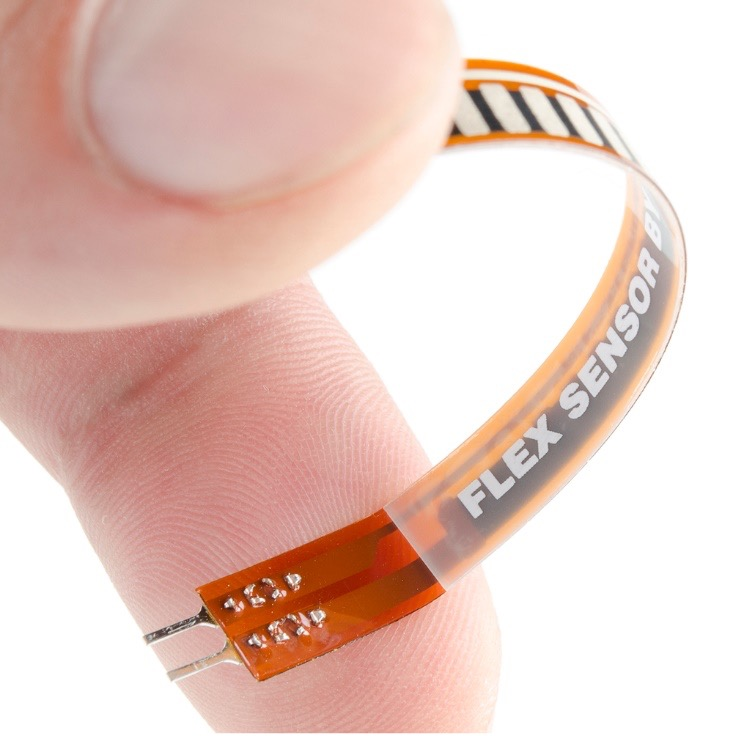
\includegraphics[width=0.8 \linewidth]{Flexsensor}}
		\caption{Flexsensor}
		\label{fig:Flexsensor}
	\end{center}
\end{figure}
\hfill \break
\textcolor{red}{\url{https://commons.wikimedia.org/wiki/File:Flex_Sensor.jpg\#/media/File:Flex_Sensor.jpg}} \\
Ein Flexsensor (Biegesensor) misst die Biegung des aus Kunststoff bestehenden 
Streifens. Die Kohlenstoffbeschichtung macht diesen dann zu einem variablen 
Widerstand. Je mehr der Flexsensor gebogen wird, desto größer wird der Widerstand. 
Die Biegung kann somit gemessen werden. Diese Information wird dann in ein 
elektrisches Signal umgewandelt, was auch für das Einlesen in den Mikrocontroller 
nötig ist. Diese Flexsensoren können beispielsweise auf einem Handschuh angenäht 
werden, um zu messen, wie sehr ein Finger abgebogen wurde. \\
\\

\subsection{Servomotor}
\label{chap:Servomotor}
\begin{figure}[H]
	\begin{center}
		\scalebox{1.0}
		{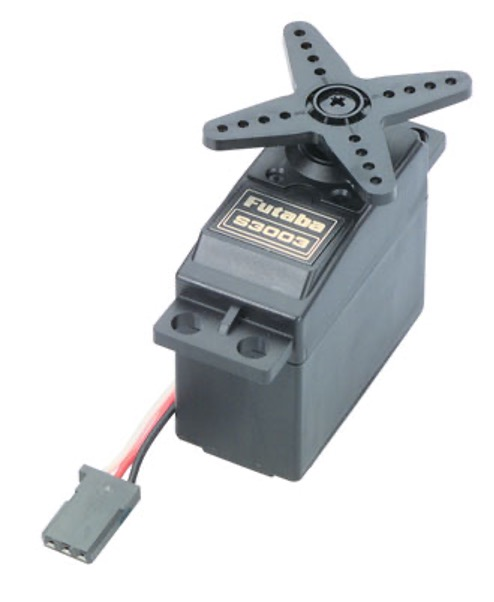
\includegraphics[width=0.8 \linewidth]{Servomotor}}
		\caption{Servomotor}
		\label{fig:Servomotor}
	\end{center}
\end{figure}
\hfill \break
\textcolor{red}{\url{https://3.bp.blogspot.com/-_Qhk9H-K3tI/UVQhc8-bxSI/AAAAAAAABT4/bWZ8dEICtZY/s640/Futaba_S3003_Servo.jpg}} \\
Ein Servomotor ist ein kleiner Elektromotor. Er besteht aus einer Steuereinheit, 
sowie einer Antriebseinheit. Ein Servo kann die Winkelposition einstellen, die 
Drehgeschwindigkeit variieren und dadurch auch die Beschleunigung beeinflussen. 
Dies funktioniert über einen Sensor, der die Positionsbestimmung durchführen kann. 
Der Servo kann über die Software festlegen, wie sich dieser drehen soll. Durch 
Sollwerte wird angegeben, wie weit sich dieser drehen soll. Für die Ansteuerung 
von einzelnen 3D-gedruckten Fingern ist ein Servo die optimale Wahl, da dieser 
die an ihm befestigten Schnüre spannen oder entlasten kann. \\
\\

\subsection{ESP-NOW \textcolor{red}{Fabian}}
\label{chap:ESP-NOW}
Das ESP-NOW Protokoll macht es möglich, dass man Daten problemlos per 
Funkstrecke versenden kann. Dabei kann dieses auf dem ESP32 und ESP8266 
verwendet werden, da nur diese dafür ausgewählt wurden. Der Hersteller 
$"$Espressif$"$ hat dieses Protokoll entwickelt. Es können bis zu 250 Bytes 
pro Sendevorgang ausgetauscht werden. Dies ist auch bis zu einer maximalen Anzahl 
von zwanzig ESP32/ESP8266 Slaves möglich. Das Mischen der beiden genannten 
Boards ist möglich. Dabei kann auch jeder der ESPs jeweils als Transmitter, 
Receiver oder Transceiver verwendet werden. Ein Vorteil dieser Übertragungsmöglichkeit 
ist, dass die dafür benötigten Bibliotheken in der Arduino IDE zu finden 
sind. Diese sind nämlich schon standardmäßig im Paket für den ESP32 und 
ESP8266 vorhanden. \\
\\
Als Erstes muss die MAC-Adresse des jeweiligen ESPs identifiziert werden. 
Bei Bedarf kann diese auch geändert werden. Es wird hierfür also kein 
Router benötigt. Diese besteht aus sechs Bytes. Angegeben wird sie im 
Hexadezimalsystem, wobei zwischen Zweierblöcken von Buchstaben und Zahlen 
jeweils ein Doppelpunkt steht. Um auf alle WIFI-Funktionen nutzen zu können, 
muss auch die Bibliothek für WIFI eingebunden werden. Wichtig ist, dass WIFI 
zuvor aktiviert wurde, da sonst keine Daten übertragen werden können. Durch 
den Aufruf der Funktion esp\_now\_init$()$ kann ESP-NOW initialisiert werden, 
mit esp\_now\_deinit$()$ kann es wieder rückgängig gemacht werden. Durch die 
Funktion esp\_now\_add\_peer$()$ können neue Geräte, an die man dann etwas sendet, 
in die Liste der Geräte aufgenommen werden. Zu beachten ist, dass Kanäle von 0 bis 14 vorhanden 
sind, wobei 0 für den aktuellen Kanal steht. Darüber wird dann auch gesendet, 
außer man stellt einen spezifischen Kanal ein, auf dem sich das lokale Gerät 
befindet. \\
\\
Um Daten zu senden, muss die Funktion esp\_now\_send$()$ aufgerufen werden. 
Dadurch können dann Daten gesendet werden. Die Funktion esp\_now\_register\_send\_cb$()$ 
ist dafür da, um die Sende-Callback-Funktion zu registrieren. Es wird ein 
Wert zurückgeliefert, der angibt, ob die Daten erfolgreich gesendet wurden oder 
nicht. Bei einem erfolgreichen Sendevorgang wird ESP\_NOW\_SEND\_SUCCESS zurückgeliefert. 
Dies passiert, wenn sie erfolgreich am MAC-Layer der Empfängerseite empfangen wurden, ansonsten 
ESP\_NOW\_SEND\_FAIL. Warum eine Fehlermeldung ausgegeben wird, kann nicht 
nur einen Grund haben. Beispielsweise existiert die angestrebte MAC-Adresse 
nicht, die Kanäle sind nicht identisch oder der Action frame geht bei der 
drahtlosen Übertragung verloren. Um doppelte Daten auszuschließen, ist es 
möglich, dass man eine Sequenznummer verwendet, um zu überprüfen, ob es eine 
fehlerbehaftete Übertragung sein könnte. Ein zu kurzes Intervall zwischen 
dem Senden der verschiedenen Daten kann dazu führen, dass eine Störung 
auftreten kann. Die Sende-Callback-Funktion kann dadurch gestört werden. Es 
sollte deshalb auf jeden Fall der Moment abgewartet werden, bis die Sende-Callback-Funktion 
eine Antwort geliefert hat. Dabei wird diese Funktion jedes Mal mit hoher 
Priorität beim Wifi-Task ausgeführt. In der Callback-Funktion sollen auf 
jeden Fall nur die wichtigsten Operationen abgearbeitet werden. \\
\\
Um Daten zu empfangen, muss die Funktion esp\_now\_register\_recv\_cb$()$ aufgerufen 
werden. Dies ist dafür verantwortlich, um die Empfangs-Callback-Funktion zu 
realisieren. Genauso, wie beim Sender, wird hierzu der WIFI-Task verwendet, 
weshalb nur die nötigsten Operationen abgearbeitet werden sollen. \\
\\
Mit der Funktion esp\_wifi\_config\_espnow\_rate$()$ kann die ESP-NOW Datenrate angegeben 
werden. Dabei muss beachtet werden, dass die gewünschte Schnittstelle bereits 
konfiguriert wurde. Eine Energiesparen Funktion kann über 
esp\_wifi\_connectionless\_module\_set\_wakre\_interval$()$ festgelegt werden. Hier 
meist durch eine Wand, in seltenen Fällen sogar durch zwei, abhängig von der Dicke 
kann man dann einstellen, wann sich der ESP einschalten soll. \\
\\
Im Freien, ohne störende Wände oder Möbel, kann ESP-NOW Daten auf jeden Fall 100 
bis 250 Meter weit übertragen. In geschlossenen Räumen funktioniert die Übertragung 
und anderen störenden Einflüssen. \footnote{\url{https://wolles-elektronikkiste.de/esp-now\#range}, (Stand: 21.02.2024)} \\
\\
Das OSI-Modell wird bei dem ESP-NOW Modell von sieben Schichten auf 
zwei reduziert. Daten müssen somit nicht den Network-Layer, den 
Transport-Layer, den Session-Layer, den Presentation-Layer und 
den Application-Layer durchlaufen. Nur der Data-Link-Layer (SLIP/PPP/MTU), 
sowie der Physical-Layer (802.11b/g/n), werden verwendet. 
Der große Vorteil liegt außerdem 
darin, dass man einige Dinge nicht berücksichtigen muss. Es gibt keine 
Paketköpfe oder Entpacker auf jeder Schicht. Dies führt zu einer schnelleren 
Reaktion, zu weniger Overhead und die Paketverluste werden dadurch in überlasteten Netzen 
reduziert. Dies führt zu einer deutlichen Verbesserung der möglichen 
Verzögerung, indem diese sehr niedrig gehalten werden kann. \footnote{\url{https://www.espressif.com/en/solutions/low-power-solutions/esp-now}, (Stand: 21.02.2024)} \\
\begin{figure}[H]
	\begin{center}
		\scalebox{1.0}
		{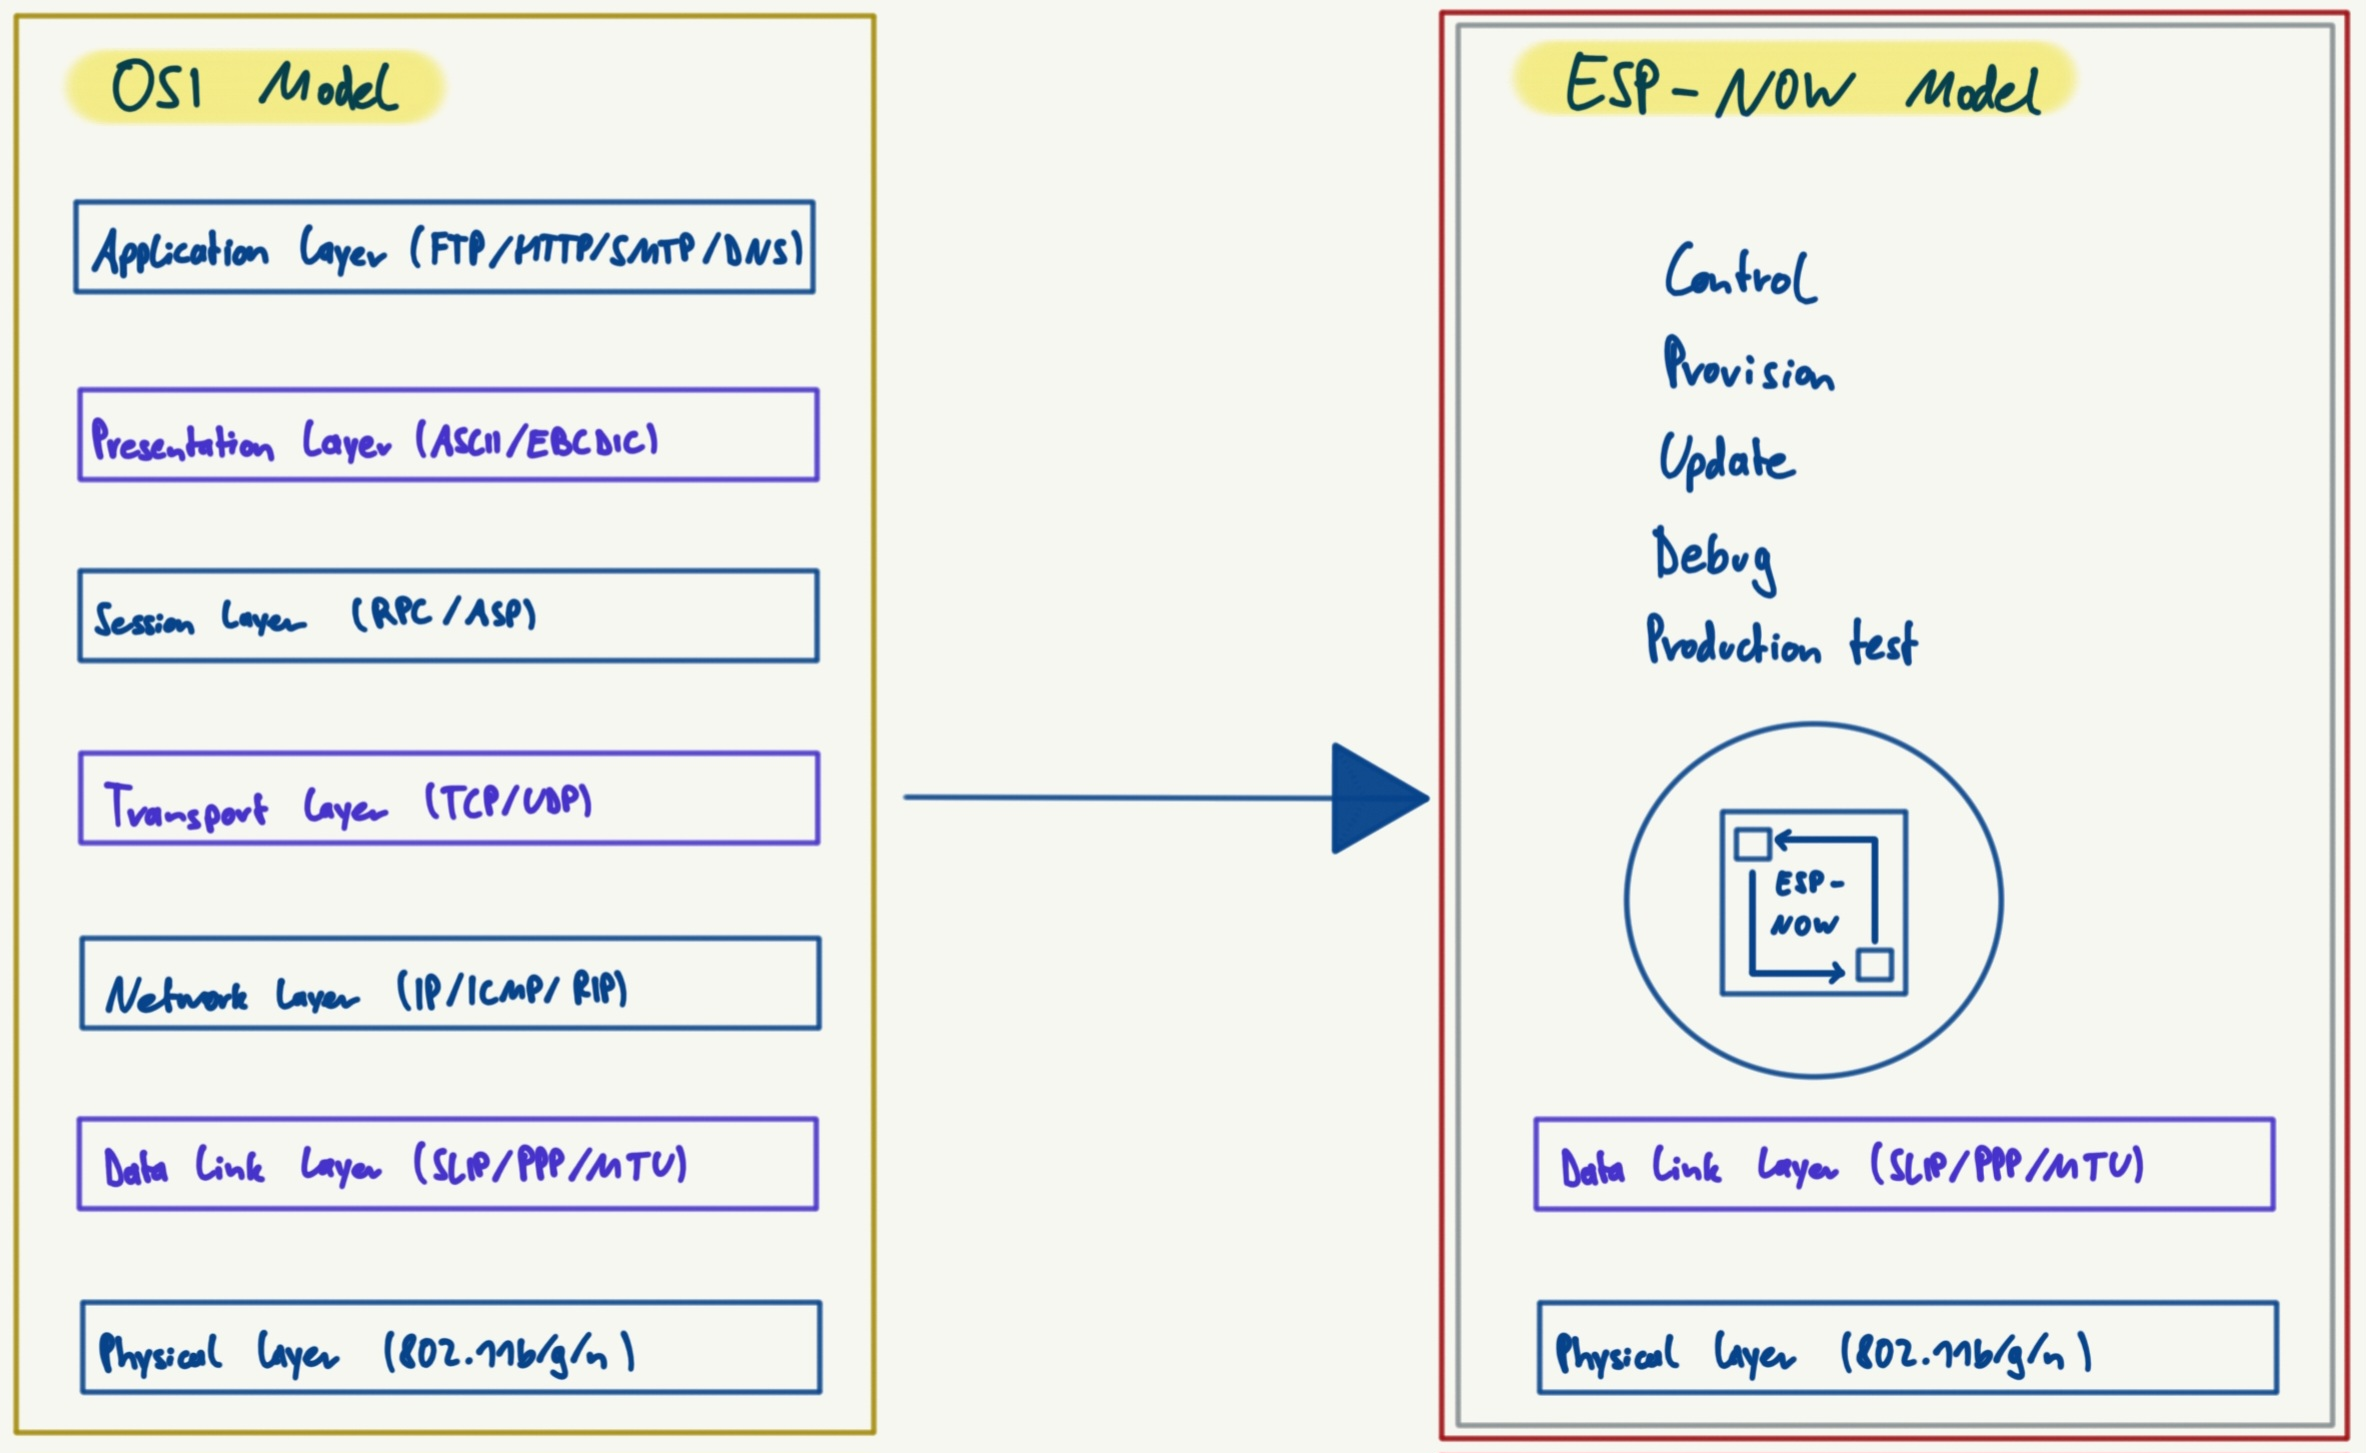
\includegraphics[width=0.8 \linewidth]{ESPNOW_Model}}
		\caption{ESPNOW - Model}
		\label{fig:ESPNOW_Model}
	\end{center}
\end{figure}

\subsubsection{OSI-Modell}
\label{chap:OSI-Modell}
Das OSI-Modell ist standardisiert und ermöglicht die Kommunikation zwischen den 
verschiedensten Computersystemen. OSI (Open Systems Interconnection) wurde von der 
ISO (International Organization for Standardization) erfunden. 
Es besteht aus 7 Schichten (application layer, presentation layer, session layer, 
transport layer, network layer, data link layer und physical layer). Wichtig ist, 
dass jede einzelne Schichte eine andere Aufgabe erfüllt. Durch das System der 
einzelnen Schichten kann die Fehlersuche vereinfacht werden, da man die jeweiligen 
durchforsten kann. Zu beachten ist allerdings, dass diese untereinander ebenfalls 
Daten austauschen und untereinander kommunizieren können. Dabei ist jede Schicht 
nach international standardisierten Protokollen definiert. Das bedeutet, dass gewisse 
Regeln zur Kommunikation eingehalten werden müssen. Dabei ist es möglich, dass sich 
ein Protokoll über mehrere Schichten verteilt. \\
\\
Beim Sender und Empfänger werden diese sieben Schichten jeweils einmal angewandt. \\
\\

\paragraph{Physical Layer}
\label{par:Physical Layer}
\hfill \break
\hfill \break
Beschreibt die mechanische und funktionale Schnittstelle zum Übertragungsmedium. Die 
Datenübertragung der physischen Geräte, wie Schalter, Kabel, usw. ist hiermit gemeint. 
Daten werden in einen Bitstrom umgewandelt. Zu beachten ist, dass das Übertragungsmedium 
an sich nicht zur 1. Schicht gehört, nur die Datenübertragung bei Einschalten des 
physischen Geräts gehört in diese.\\

\paragraph{Data Link Layer}
\label{par:Data Link Layer}
\hfill \break
\hfill \break
Beschreibt die Sicherungsschicht, die eine stabile und funktionierende Verbindung 
zwischen Endgerät und Übertragungsmedium herstellt. Der Data Link Layer verarbeitet 
Pakete vom Network Layer, spaltet diese in kleinere Teile namens Frames und ist für 
den Datentransfer zwischen zwei Geräten im selben Netzwerk verantwortlich. Die 
physikalische Adressierung von Datenpaketen wird hier durchgeführt. Außerdem werden 
auch eine Fehlererkennung, Fehlerbehebung und Datenflusskontrolle angewandt. \\

\paragraph{Network Layer}
\label{par:Network Layer}
\hfill \break
\hfill \break
Beschreibt den regulierten Datentransfer zwischen zwei verschiedenen Netzwerken. Hier 
werden einzelne Segmente auf dem Sendergerät von dem Transport Layer in Fragmente 
aufgeteilt und auf dem Empfängergerät dann wieder zusammengefügt. Die logische Adressierung 
findet ebenfalls statt. \\

\paragraph{Transport Layer}
\label{par:Transport Layer}
\hfill \break
\hfill \break
Beschreibt das Bindeglied zwischen den transportorientierten und den anwendungsorientierten 
Schichten. Wie immer, werden die Daten in kleinere Bestandteile zerlegt. Header-Informationen 
und eine Fehlerkontrolle werden von den Segmenten beinhaltet, falls nicht alle Daten 
erfolgreich angekommen sind oder fallengelassen wurden, kann dies hilfreich sein. \\

\paragraph{Session Layer}
\label{par:Session Layer}
\hfill \break
\hfill \break
Beschreibt die Verbindung zwischen den Endsystemen. Session nennt man den zeitlichen 
Bereich zwischen dem Starten und Beenden der Kommunikation. Wichtig ist auch, dass 
dieser Layer dafür verantwortlich ist, dass genug lange Daten übertragen werden können 
und die Verbindung nicht schon zuvor beendet wird. Für die Effizienz soll allerdings 
nach einem abgeschlossenen Vorgang die Verbindung unterbrochen werden. \\

\paragraph{Presentation Layer}
\label{par:Presentation Layer}
\hfill \break
\hfill \break
Beschreibt die Aufbereitung der Daten, sodass der Nutzer diese verstehen kann. Damit 
ist gemeint, dass beispielsweise verschlüsselte Daten zuerst entschlüsselt werden 
müssen, bevor sie der Nutzer verstehen kann. Die Komprimierung und Dekomprimierung 
von Daten werden hier auch durchgeführt. \\

\paragraph{Application Layer}
\label{par:Application Layer}
\hfill \break
\hfill \break
Beschreibt die Bereitstellung von Funktionen für Anwendungen und die Verbindung zu 
den unteren Schichten. Die Dateneingabe und Datenausgabe werden hier ebenfalls 
durchgeführt. Softwareanwendungen sind auf den Application Layer angewiesen (http, SMTP, …). 
Diese Protokolle sind für die Kommunikation notwendig und standardisiert. \\

\paragraph{ESP-NOW Schichten}
\hfill \break
\hfill \break
Es gibt bei ESP-NOW zwei Schichten, den Data Link Layer und den Physical Layer 
(siehe \autoref{chap:OSI-Modell}). Dabei beruht der Physical Layer auf dem IEEE 802.11b/g/n Standard. 
Da jedoch nicht so viele Schichten, wie bei dem OSI-Modell vorhanden sind, gibt es 
mehrere Möglichkeiten, wo Fehler liegen können und es ist nicht so leicht den Fehler 
an der richtigen Stelle zu suchen. \\

\paragraph{IEEE 802.11b/g/n Standard}
\label{par:802.11b/g/n Standard}
\hfill \break
\hfill \break
Es ist ein internationaler Standard für die drahtlose Kommunikation, der von 
Electrical and Electronics Engineers (IEEE) entwickelt wurde. Besonders wird Wert auf 
die geringe Datenrate und dem daraus folgend geringen Stromverbrauch Wert gelegt. Der 
802.11b Standard hat eine maximale Datenübertragungsrate von 11Mbit/s, 802.11g eine 
maximale Datenübertragungsrate von 54Mbit/s und 802.11, kann bis zu 600Mbit/s übertragen. 
Der letztgenannte Standard ist der einzige, der auch das 5GHz-Band nutzen kann, alle 
drei können jedoch das 2,4GHz-Band zum Datenaustausch verwenden.  \\
\\
\begin{figure}[H]
	\begin{center}
		\scalebox{0.8}
		{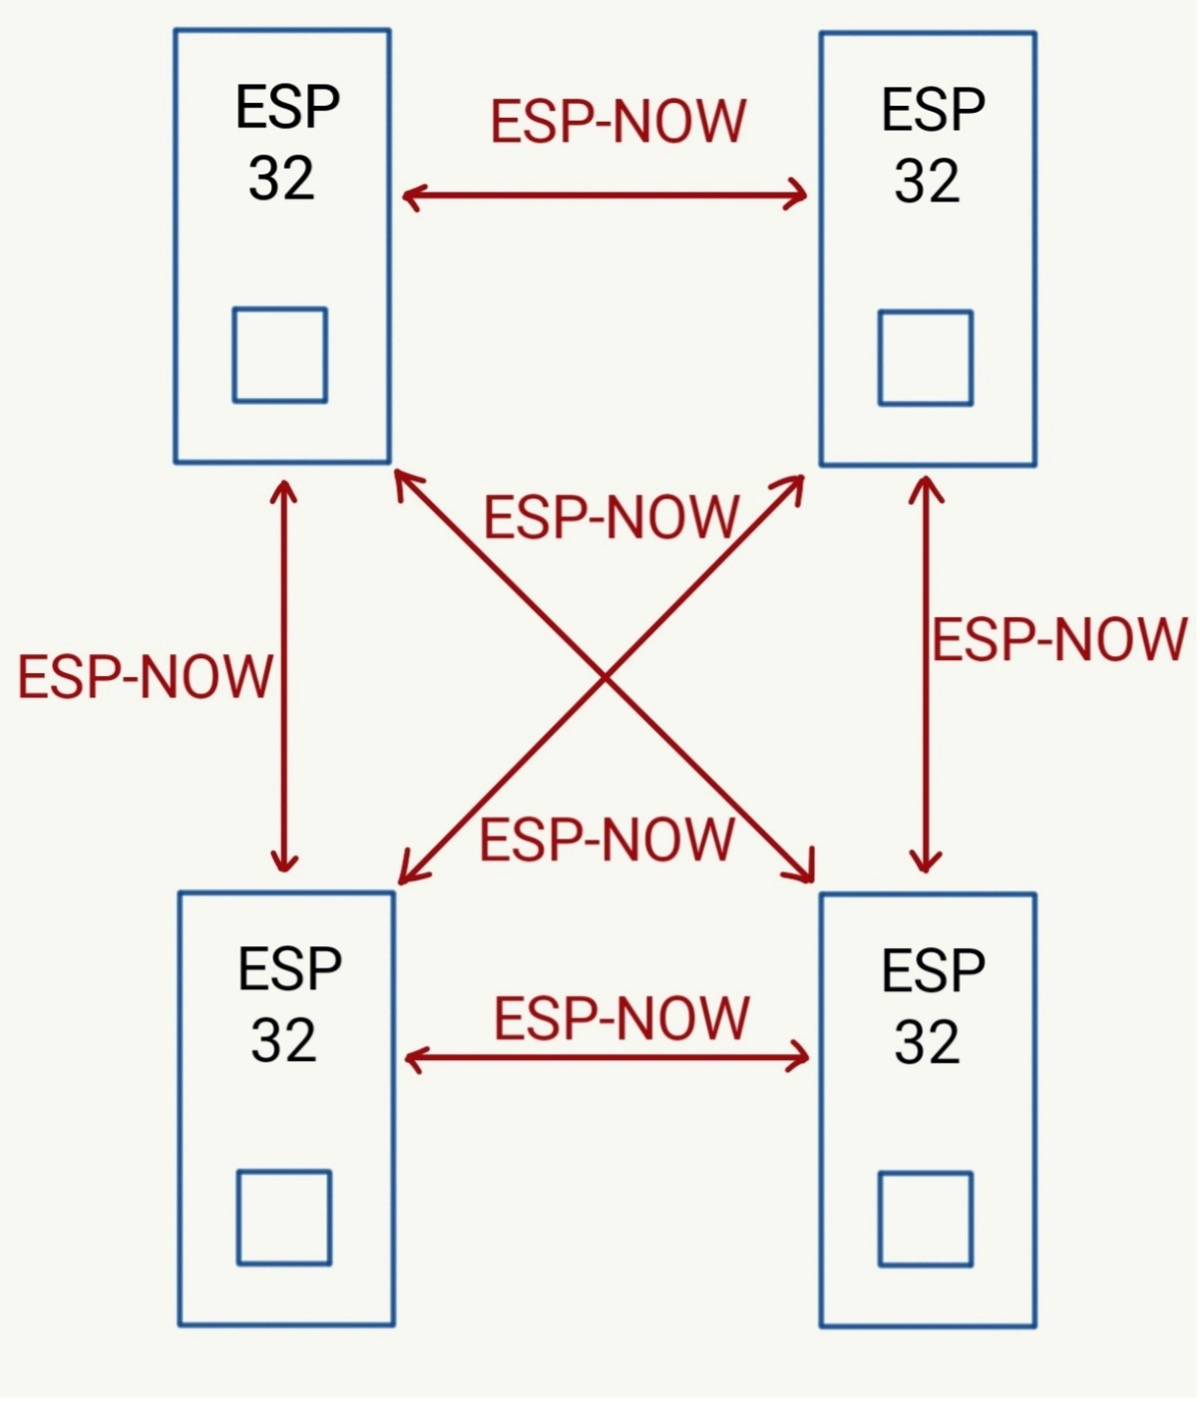
\includegraphics[width=0.8 \linewidth]{ESP_NOW_Theorie}}
		\caption{ESPNOW - Theorie}
		\label{fig:ESP_NOW_Theorie}
	\end{center}
\end{figure}
\hfill \break

\subsection{OPV Technologien \textcolor{red}{Laci}}
\label{chap:OPV Technologien}
Ein Operationsverstärker, kurz OPV, ist ein analoger Gleichspannungsverstärker, der sich durch seine üblicherweise sehr hohe 
Verstärkung auszeichnet. Der elektroische Grundbaustein ist ein Differenzverstärker, der durch äußere Beschaltungen angepasst werden kann.
In der grundlegendsten Funktion, verstärkt ein OPV die Differenz der beiden Eingangsspannungen am $"$+$"$ und $"$-$"$ Anschluss. Das Ergebnis
dieses Verstärkungsprozesses wird anschließend über $"$Vout$"$ ausgegeben. \\
\\
Operationsverstärker können mit einem sogenannten $"$Single-Supply$"$ oder $"$Dual-Supply$"$ versorgt werden. Dies bezieht sich auf
die Art der Versorgungsspannung. \\
\\
\subsubsection{Single-Supply}
Bei dieser Art der Versorgung, wird ausschließlich eine positive Spannung und das Groundpotential genutzt. Das bedeutet, dass der OPV
theoretisch einen maximalen Ausgangsbereich von GND bis VCC haben kann. Negative Spannungen können nicht ausgegeben werden. \\
\\

\subsubsection{Dual-Supply}
Beim Dual-Supply Betrieb, wird der OPV von einer positiven und negativen Spannung versorgt. Das bedeutet, dass der OPV nun die Fähigkeit
besitzt auch negative Spannungen auszugeben und der Ausgangsspannungsbereich somit größer als beim Single-Supply ist.

\subsubsection{Rail-to-Rail Technologie}
Hat ein OPV die sogenannte $"$Rail-to-Rail Technologie$"$, so ist die Rede von Spannweite des Ausgangsspannungsbereichs. Bei diesem Feature
ist der Operationsverstärker dazu fähig fast bis auf das positive und negative Versorgungspotential Spannung auszugeben. Dies ist oft 
von Vorteil, da dadurch die Versorgungsspannungen nicht übermäßig hoch sind und somit die Schaltungen mit niedrigeren Spannungen arbeiten
kann. Dies ist auch für die Benutzer der entsprechenden Endgeräte sicherer.\\
\\
In \autoref{fig:RAILtoRAIL_OPV} sind die Ausgangsspannungsbereiche eines normalen OPVs, in blau, und eines OPVs mit Rail-to-Rail Technologie,
in Orange, dargestellt. \\
\begin{figure}[H]
	\begin{center}
		\scalebox{1.2}
		{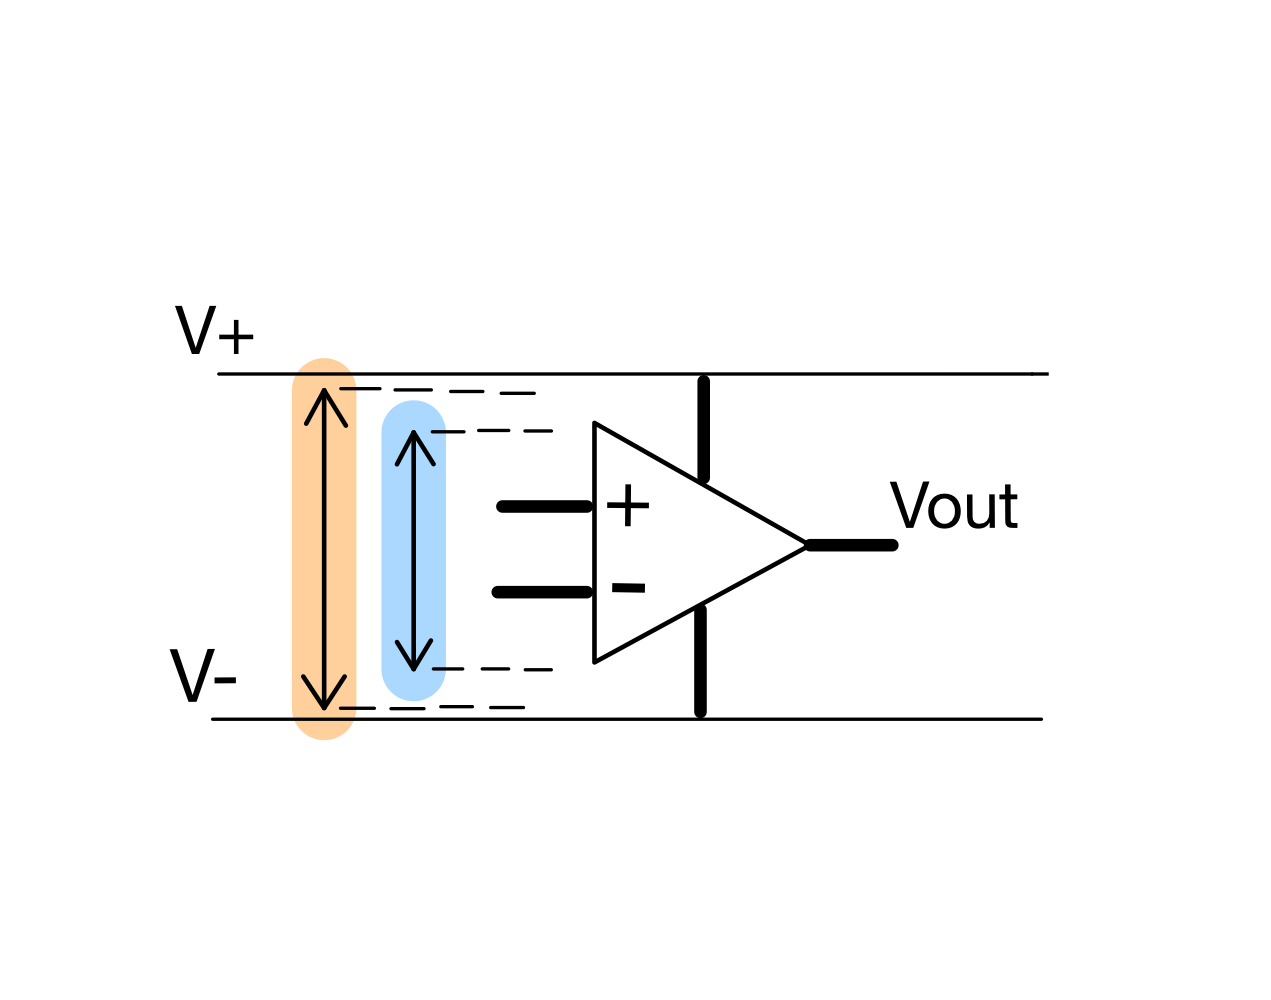
\includegraphics[width=0.8 \linewidth]{RAILtoRAIL_OPV}}
		\caption{OPV Ausgangsspannungbereiche}
		\label{fig:RAILtoRAIL_OPV}
	\end{center}
\end{figure}

\subsection{Analog-Digital-Wandler}
\label{chap:Analog-Digital-Wandler}
\begin{figure}[H]
	\begin{center}
		\scalebox{1.2}
		{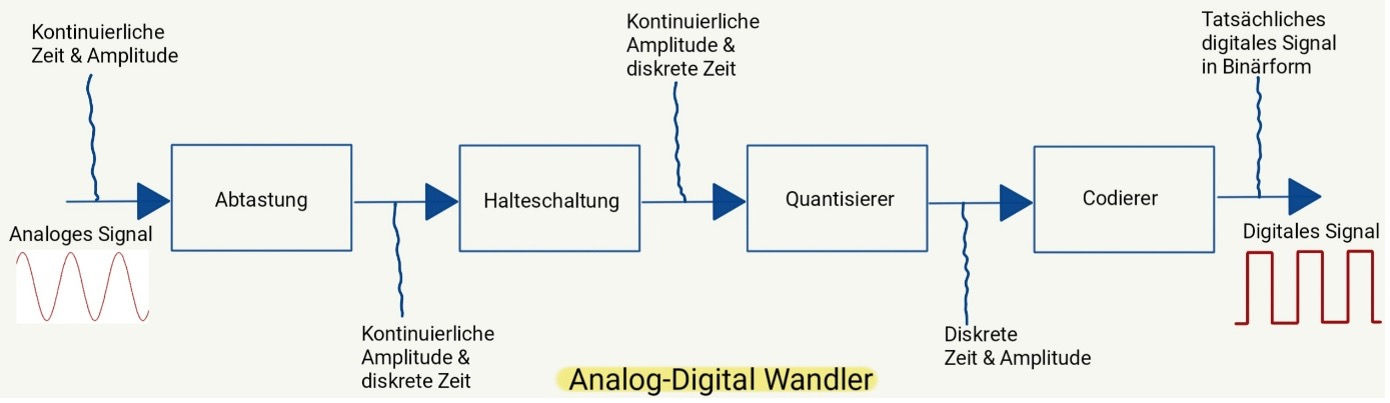
\includegraphics[width=0.8 \linewidth]{ADC_Blockschaltbild}}
		\caption{Blockschaltbild Analog-Digital-Wandler}
		\label{fig:ADC_Blockschaltbild}
	\end{center}
\end{figure}
\hfill \break
Ein ADC (Analog-Digital-Converter) wandelt kontinuierliche analoge Signale 
(physikalische Größen) in digitale Signale um. Dies ist notwendig, damit ein 
Prozessor die Werte verarbeiten kann. Deshalb kommen ADCs in elektronischen 
Schaltungen häufig vor. \\
\\
Abtastung: Es werden kontinuierliche analoge Signale mit einer bestimmten 
Abtastrate abgetastet. Das kontinuierliche Signal wird hierbei zu einem 
zeitdiskreten, wobei die Amplitude stets kontinuierlich bleibt. \\
\\
Halteschaltung: \\
Die nach der Abtastung vorhandenen Messwerte werden in der Halteschaltung so 
lange zurückgehalten, bis ein neuer die Halteschaltung erreicht. \\
\\
Quantisierer: \\
Die Messwerte werden hier in diskrete Amplitudenwerte aufgeteilt. Das Signal 
ist ab dem Quantisierer zeitdiskret und besitzt nun eine diskrete Amplitude. \\
\\
Codierer: \\
Der Codierer wandelt dann das quantisierte Signal in ein binäres um. Am Ende ist 
dann ein digitales Signal in Binärform vorhanden. \\
\\

\subsection{Multiplexer}
\label{chap:Multiplexer}
Untenstehend kann man noch anhand einer einfachen Logikschaltung eines 2-zu-1 
Multiplexers die Funktionsweise eines Multiplexers. Grundsätzlich wird über elektrische 
Signale einer von mehreren Eingangssignalen an den Ausgang durchgeschaltet. Meist 
funktioniert dies durch Halbleiterelemente. Das Steuersignal s schaltet noch zusätzlich. \\
\\
\begin{figure}[H]
	\begin{center}
		\scalebox{1.2}
		{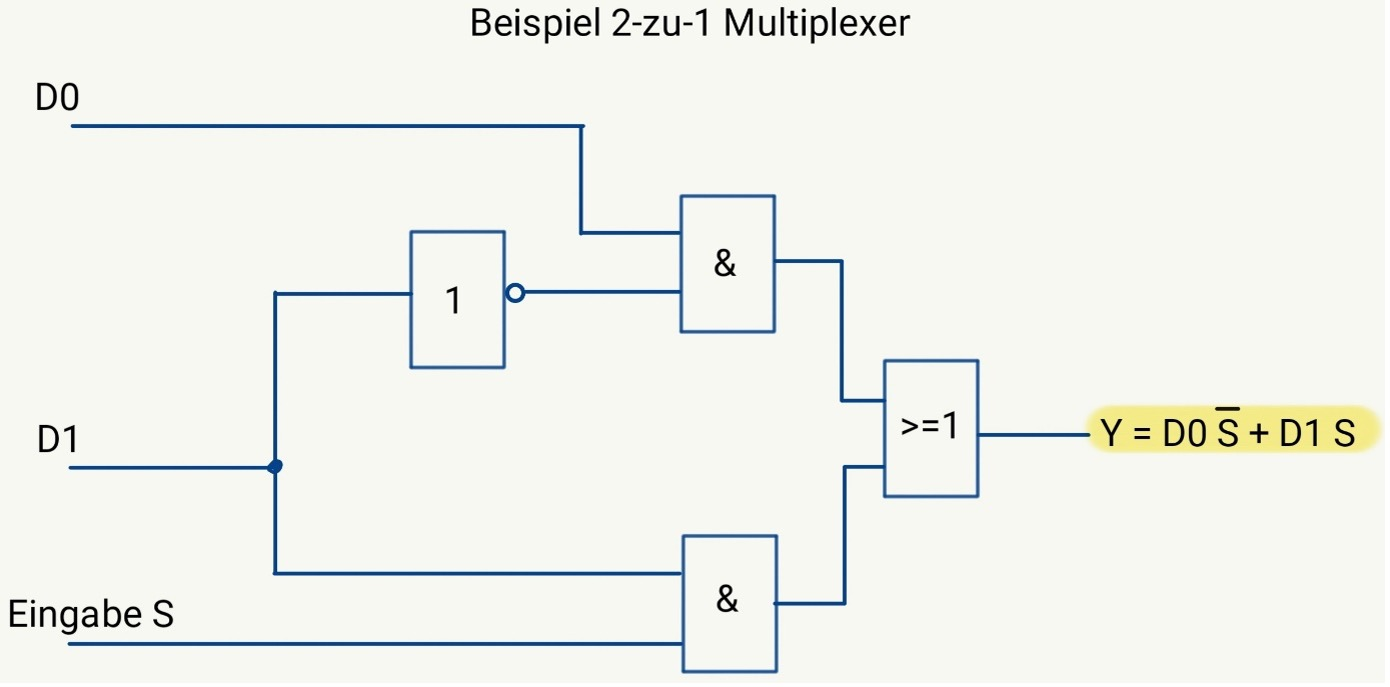
\includegraphics[width=0.8 \linewidth]{Multiplexer_Beispiel}}
		\caption{Multiplexer Beispiel}
		\label{fig:Multiplexer_Beispiel}
	\end{center}
\end{figure}
\hfill \break

\subsection{PWM-Signale}
\label{chap:PWM-Signale}

\subsection{I2C Funktionsweise}
\label{chap:I2C Funktionsweise}
\textbf{I2C Funktionsweise}
\\
I2C beschreibt eine Möglichkeit, über die zwei verschiedene Geräte miteinander 
kommunizieren können. Die Daten werden hintereinander gesendet und dies über zwei 
Datenleitungen. Es kann dabei mit bis zu 128 Teilnehmern kommuniziert werden. Am Ende 
interpretiert der I2C-Bus die Daten und steuert den Ablauf. Bei unserem Projekt ist 
der ESP32 der Master und die Flexsensoren beispielsweise die Slaves. Der Master ist 
dann der wichtige Bestandteil, da dieser für alle anderen Slaves derjenige ist, der 
sagt, was welches Bauteil machen soll. Dabei hängen alle Geräte beziehungsweise 
Bauteile an zwei Leitungen. Eine heißt SDA (serial data) und ist für die serielle 
Übertragung der Daten verantwortlich. Jedoch ist zu erwähnen, dass diese bidirektional 
benutzt wird. Das heißt es kann in beide Richtungen gesendet werden (Master zum 
Slave und umgekehrt). Es muss aber der Master regeln, also entweder Daten senden 
oder welche von einem Slave anfordern. Die zweite Leitung heißt SCL (serial clock) 
und ist für den Takt zuständig, der für alle per I2C verbundenen Geräte gilt. Es 
wird also ein synchroner Bus verwendet. \\
\\
\textbf{Beispiel Protokoll I2C}
Die Daten sind grundsätzlich in Datenpaketen verpackt, jedes besteht aus 1 Byte. 
Wenn nichts kommuniziert wird, dann hat SDA und SCL den Wert 1. Nachdem eine 
Start-Condition gesendet wurde, durch die alle Slaves wissen, dass sie nun auf den 
Master jederzeit reagieren sollen, wird die Adresse des Slaves gesendet, mit dem 
nun Daten ausgetauscht werden sollen. 7 Bit werden hierfür standardmäßig verwendet. 
Danach wird ein weiteres Bit gesetzt. Dieses kann den Wert 0, was Schreiben bedeutet, 
oder 1, was lesen bedeutet, haben. Nun ist der Slave an der Reihe. Dieser muss 
ebenso 0, wenn die Kommunikation bereitsteht, an den Master zurücksenden. Der Master 
sendet dann oder empfängt Daten vom Slave. Sobald alle Daten versendet wurden, 
kommt die Bestätigung. Der ganze Vorgang des Senden und Empfangens wird am Ende 
dann durch die Stop-Condition beendet. SDA wird hier auf 1 gesetzt, währenddessen 
SCL auch den Wert 1 besitzt. \\
\\
\textcolor{red}{http://fmh-studios.de/theorie/informationstechnik/i2c-bus/}
\\
\begin{figure}[H]
	\begin{center}
		\scalebox{1.2}
		{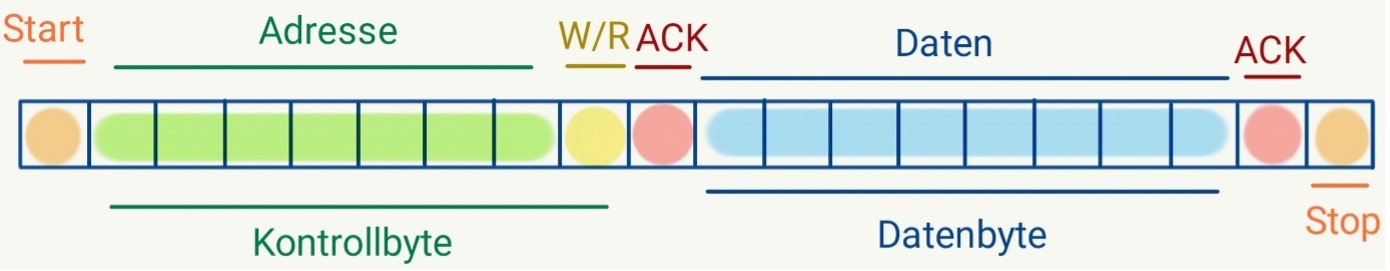
\includegraphics[width=0.8 \linewidth]{I2C}}
		\caption{I2C Adressierung}
		\label{fig:I2C}		
	\end{center}
\end{figure}
\hfill \break

\subsection{UART Funktionsweise}
\label{chap:UART Funktionsweise}
Der Arduino, beziehungsweise der ESP, werden über die serielle Verbindung UART 
(Universal Asynchronous Receiver and Transmitter) vom Computer angesprochen. 
Dabei stellt diese Verbindung eine asynchrone Datenübertragung mit fester Baudrate, 
Datenbits, Paritätsbits und Stoppbits dar. Es sind zwei Datenleitungen vorhanden, wobei 
eine für das Senden (TX) und die andere für das Empfangen (Rx) von Daten zuständig ist. 
Die Start- und Stopbits geben an, wann gesendet werden soll und wann dies nicht 
mehr geschehen soll. Sobald der Sender ein Startbit erhält, beginnt die Übertragung 
der Daten, aber beim Empfangen des Stopbit wird diese unterbrochen. Es wird 
dadurch keine Clock benötigt, da die Baud Rate dies regelt, allerdings ist zu 
beachten, dass diese maximal 10\% von jeder des anderen Geräts abweichen darf. 
Die Baud Rate gibt an, wie viele Symbole pro Sekunde übertragen werden. Dabei 
kann ein Symbol ein einzelnes Bit oder eine Gruppe von Bits sein. Die Baudrate 
gibt also an in welchem Abstand jeweils ein Symbol gesendet wird (1s/Baudrate) 
oder eben im Umkehrschluss auch, wie viele Symbole pro Sekunde gesendet werden 
(Baudrate/1s). \\
\\
\textbf{Beispiel Protokoll für 8-Bit Packet}
Es ist ein Startbit vorhanden (LOW), dann noch 8 Datenbits (inklusive einem 
Paritybit, das Fehler identifizieren kann) und ein oder zwei Stopbits (HIGH). 
Zur Kontrolle, ob es eine gerade oder ungerade Anzahl von Highbits gibt, wird 
ein Paritybit mitgesendet, das angibt, ob die Anzahl dieser gerade oder ungerade 
ist. Es gibt klarerweise keine hundertprozentige Sicherheit, aber man kann sich 
mehr auf die Nutzbarkeit der Daten verlassen. Bei der UART-Kommunikation bedeutet 
ein Paritybit von 0 (odd), dass die Summe der Highbits eine ungerade Zahl ist. Ein 
Paritybit von 1 (even) hingegen zeigt an, dass die Summe der Highbits eine gerade 
Zahl ist. Üblicherweise werden zwei Stopbits am Ende einer Übertragung gesendet, 
um eine verlängerte Ruhephase zu gewährleisten. 
Dies führt zu einer stabileren Synchronität und Erhöhung der Robustheit gegen 
Signalstörungen. Bei UART wird das LSB (least significant bit) immer ganz rechts 
in den Daten gefunden. Sollte das Paritybit nicht stimmen, dann wird vom 
Empfänger an den Sender eine Anfrage mit der Bitte um erneutes Senden gesendet, 
da der Datensatz nicht stimmt. \\

\textcolor{red}{https://edistechlab.com/wie-funktioniert-uart/?v=fa868488740a}

\begin{figure}[H]
	\begin{center}
		\scalebox{1.0}
		{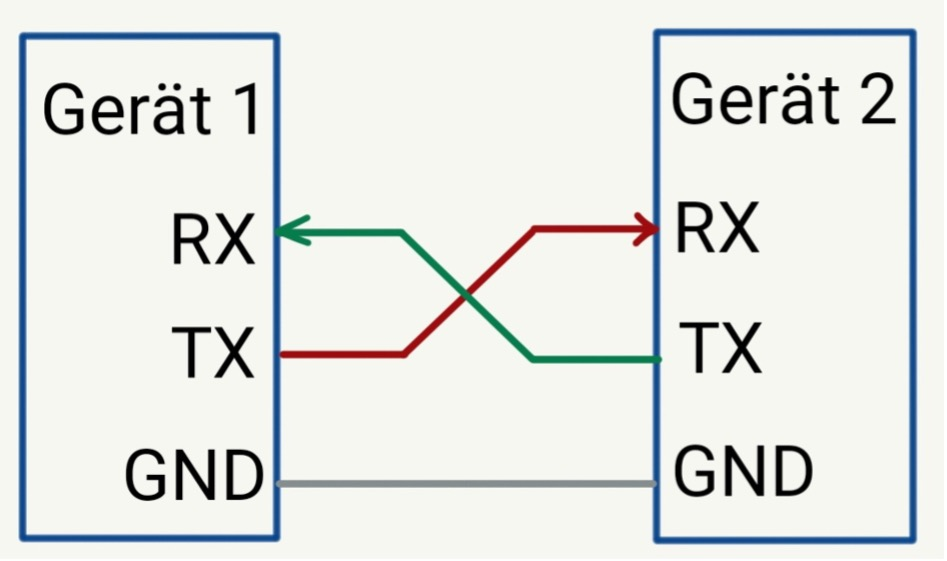
\includegraphics[width=0.8 \linewidth]{UART}}
		\caption{UART erklärendes Diagramm}
		\label{fig:UART}		
	\end{center}
\end{figure}
\hfill \break

\subsection{WiFi}
\label{chap:WiFi}
\begin{figure}[H]
	\begin{center}
		\scalebox{1.2}
		{
\includegraphics[width=0.8 \linewidth]{WiFi_Logo}}
		\caption{WiFi Logo}
		\label{fig:WiFi_Logo}
	\end{center}
\end{figure}
\hfill \break
\textcolor{red}{\url{https://commons.wikimedia.org/wiki/File:WiFi_Logo.svg\#/media/Datei:WiFi_Logo.svg}}
WIFI (Wireless Fidelity) ist eine Technologie zur Verbindung von drahtlosen Netzwerken. Es wird 
hauptsächlich dazu verwendet, um einen Zugang zum Internet herzustellen. Mobile Geräte werden meistens 
über WIFI mit dem Internet oder untereinander verbunden. WLAN (Wireless Local Area Network) ist dabei 
der Name für die lokale drahtlose Verbindung der Geräte innerhalb des lokalen Netzwerkes. Es können 
Datenpakete gesendet und empfangen werden. Der Vorteil dieser drahtlosen Verbindung liegt darin, dass 
die Geräte keine Verbindung per Datenkabel benötigen, sondern auch innerhalb einer bestimmten Reichweite 
überall miteinander kommunizieren können. Die Reichweite von WIFI kann dabei von verschiedenen Faktoren 
vermindert werden, wie beispielsweise durch Wände. \\
\\

\newpage
%--------------------------------------------------------------------------
%--------------------------------------------------------------------------

\section{Grundlegende Systemkonzepte}
\label{chap:Grundlegende Systemkonzepte}

\subsection{Gesamtsystemkonzept}
\label{chap:Gesamtsystemkonzept}

\subsubsection{Systembeschreibung}

	\begin{figure}[H]
		\begin{center}
			\scalebox{1.2}
			{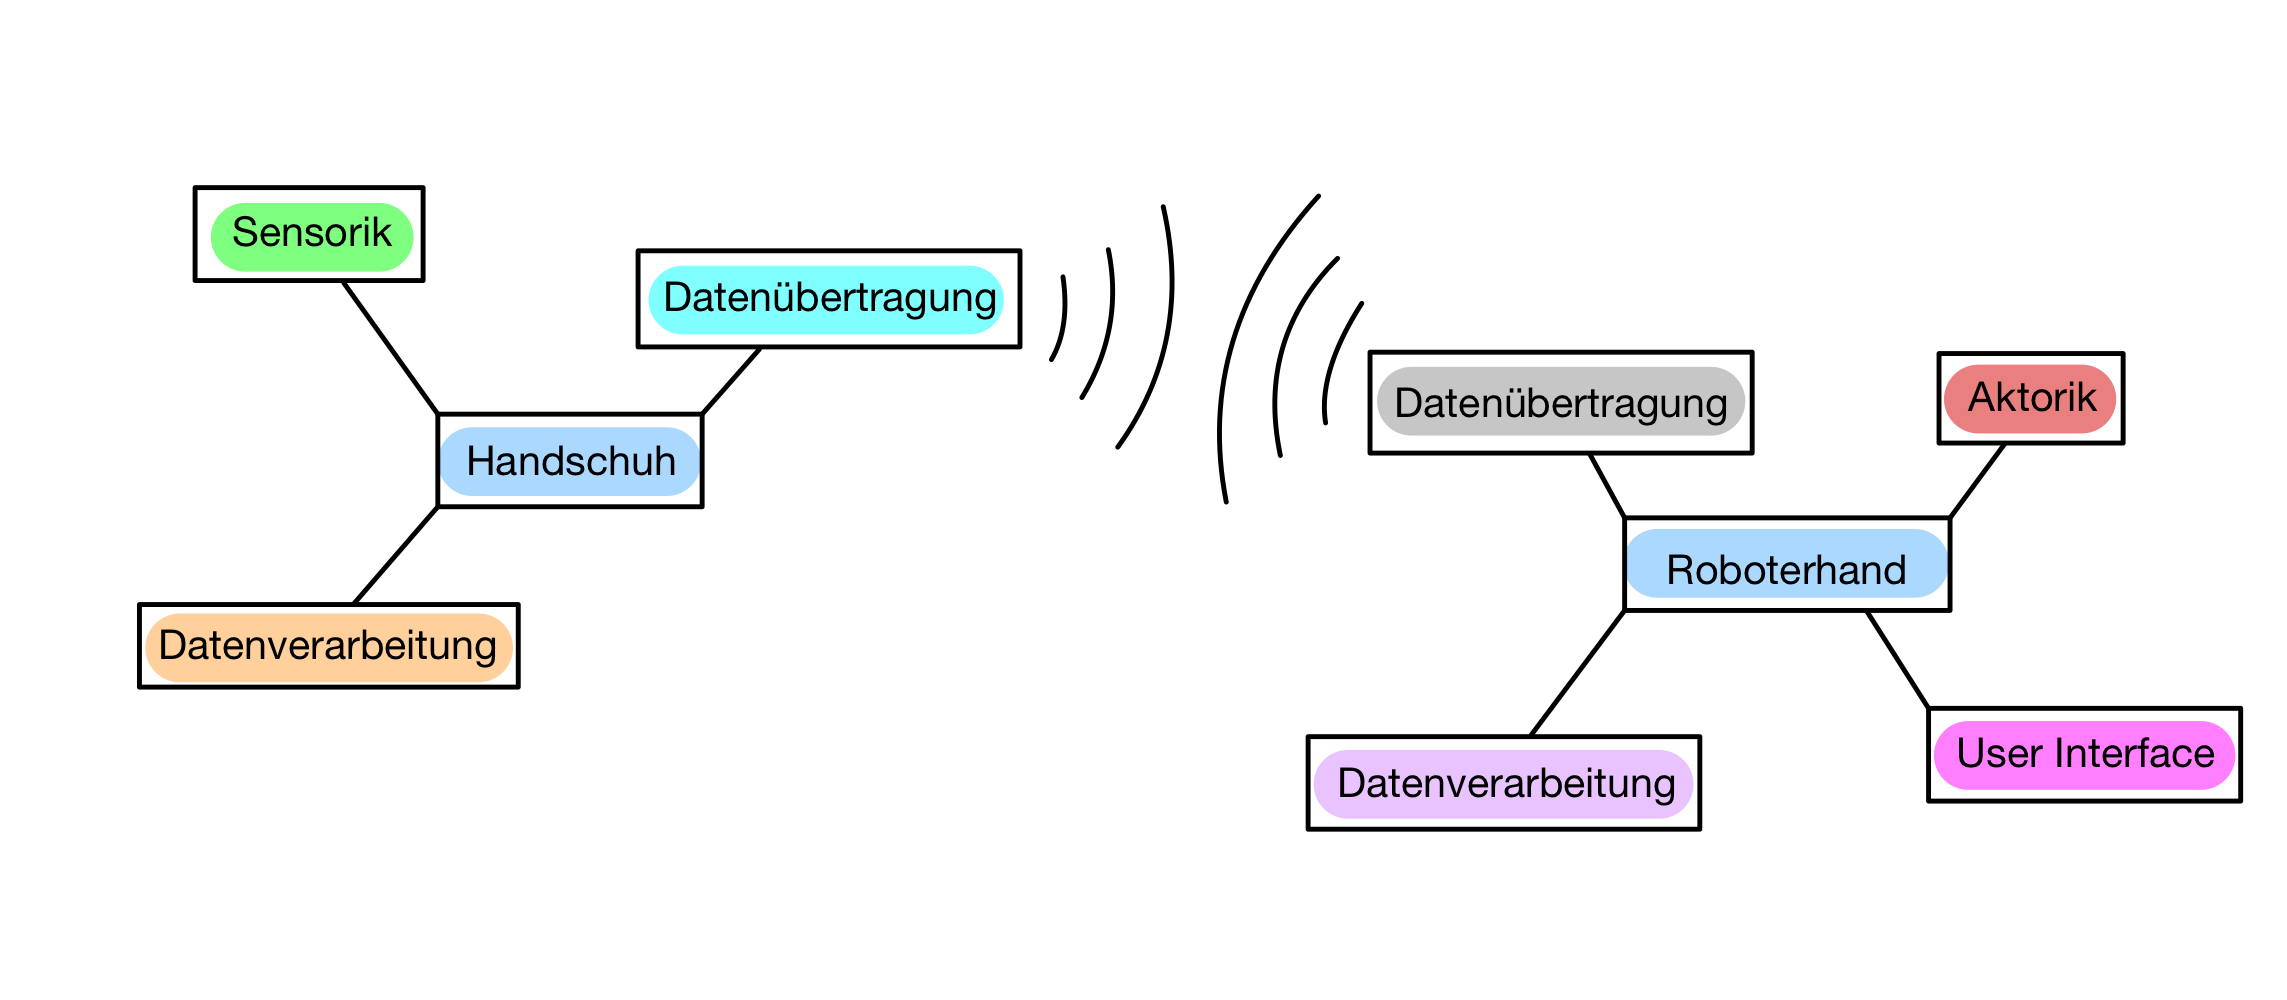
\includegraphics[width=0.8 \linewidth]{Blockschaltbild_Gesamtsystem}}
			\caption{Blockschaltbild des Gesamtsystems}
			\label{fig:Blockschaltbild_Gesamtsystem}		
		\end{center}
	\end{figure}

Das Gesamtsystem ist in \autoref{fig:Blockschaltbild_Gesamtsystem} grafisch veranschaulicht. Die linke Hälfte zeigt das Konzept des 
Handschuhs (Eingabe) und die rechte Hälfte die Roboterhand (Ausgabe). Die grundlegende Konzeptionierung der Bewegungserfassung 
besteht darin, dass mithilfe von Sensoren die Fingerbeugung aller fünf Finger gemessen wird. Anschließend werden die Sensordaten
ausgewertet und verarbeitet. Die resultierenden Informationen werden folglich über eine drahtlose Verbindung an das zweite 
Subsystem, nämlich der Roboterhand, übertragen. Dort wird das Gesendete empfangen, weiterverarbeitet und interpretiert. Die Aktorik
setzt die digitalen Anweisungen in mechanische Bewegungen um, wodurch die Roboterhand gesteuert wird. Im Ausgabesystem ist auch 
ein User-Interface enthalten. Die diversen Funktionen werden in späteren Punkten näher erläutert.

\subsection{Eingabesubsystem}
\label{chap:Eingabesubsystem}

	\begin{figure}[H]
		\begin{center}
			\scalebox{0.8}
			{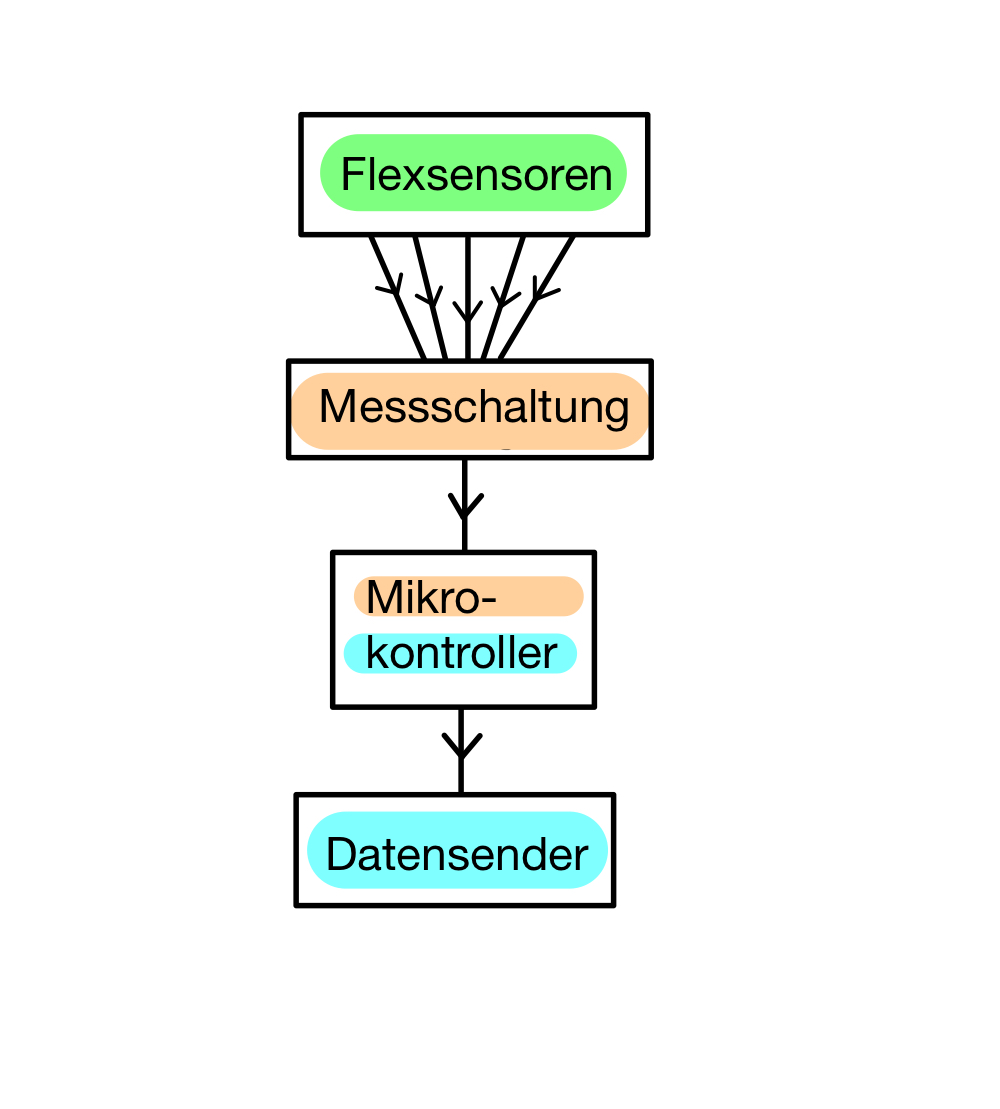
\includegraphics[width=0.8 \linewidth]{Blockschaltbild_Handschuhsystem}}
			\caption{Blockschaltbild des Eingabesubsystems}
			\label{fig:Blockschaltbild_Handschuhsystem}			
		\end{center}
	\end{figure}

Der Handschuh ermöglicht dem Benutzer die Roboterhand zu steuern. Dies geschieht 
durch Flexsensoren, die an den Fingern des Handschuhs angebracht sind. Wird ein 
Finger gebeugt, so ändert sich der Widerstandswert des Sensors. Diese Änderungen 
werden von einem Mikrokontroller erfasst, der per Kabel über UART die Werte 
kontinuierlich ausliest. Anschließend wird die kabellose Übertragung über den 
Funkstandard ESP-NOW realisiert. Das Senden an die Roboterhand wird vorbereitet. 
Damit der Handschuh funktioniert, bedarf es einer Spannungsversorgung. Diese wird 
in Form einer Batterie oder eines Akkus vorgesehen sein, funktioniert aber allenfalls 
über ein USB-C Kabel. Für einen möglichen stationären Betrieb kann der Handschuh 
auch mit einem Netzteil betrieben werden. Die Passform des Handschuhs soll 
möglichst komfortabel sein, um eine möglichst lange Benützung zu ermöglichen. 
Dies setzt eine gut überlegte Integration der Elektronik voraus. Die Flexsensoren 
sollen fest auf dem Handschuh befestigt sein. Die Widerstandswerte sind ansonsten 
bei jedem Mal biegen unterschiedlich, wenn die Flexsensoren nicht an einer Stelle 
am Handschuh bleiben, sondern sich verschieben. Diese Montage wird bei diesem 
Projekt auch bestmöglich beachtet. Der Handschuh ist so gebaut, dass er auch von 
Personen ohne elektronische Ausbildung und ohne Vorwissen bedient werden kann. 
Das liegt daran, dass nur die Finger gebeugt oder gestreckt werden müssen. Jede 
Handbewegung kann also gemacht werden, die Werte werden per Software automatisch 
richtig verarbeitet. \\

\subsection{Ausgabesubsystem}
\label{chap:Ausgabesubsystem}

\begin{figure}[H]
	\begin{center}
		\scalebox{0.8}
		{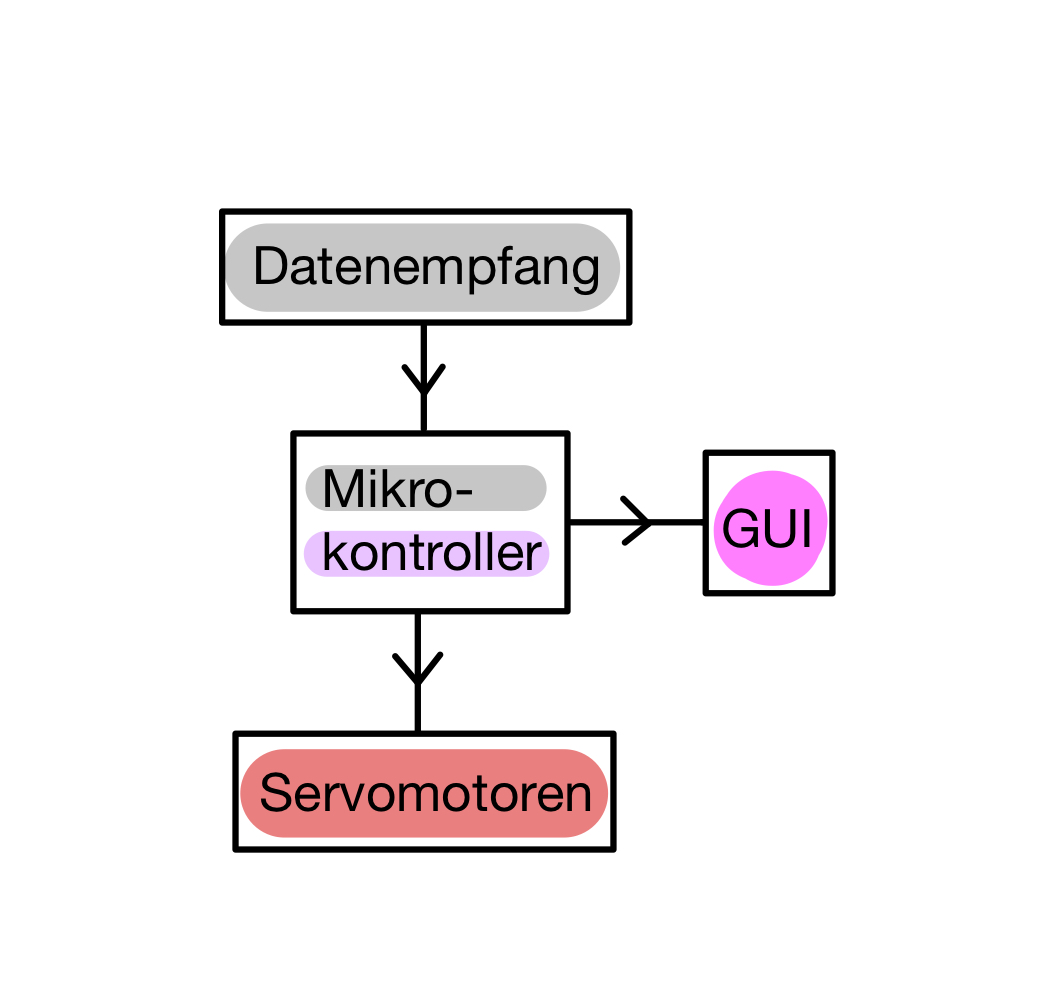
\includegraphics[width=0.8 \linewidth]{Blockschaltbild_Roboterhandsystem}}
		\caption{Blockschaltbild des Ausgabesubsystems}
		\label{fig:Blockschaltbild_Roboterhandsystem}		
	\end{center}
\end{figure}

Sind die Daten des Eingabesubsystems empfangen, müssen diese in ein geeignetes Format für die Steuerung der Aktorik, also den Servomotoren,
umgewandelt werden. Dies geschieht mit dem Mikrokontroller. Angebunden an das Ausgabesubsystem, ist ein Graphical-User-Interface, 
welches in \autoref{chap:User Interface} näher erklrärt wird. \\

\newpage
%--------------------------------------------------------------------------
%--------------------------------------------------------------------------
\section{Mechanische Realisierung}
\label{chap:Mechanische Realisierung}

\subsection{Handschuh \textcolor{red}{Amir}}
\subsubsection{\textcolor{purple}{Platzhalter für diverse Unterpunkte von Amir}}


\newpage
\subsection{Roboterhand \textcolor{red}{Amir}}
\subsubsection{Der Grundgedanke}
Der Grundgedanke der Mechanik in der Roboterhand ist es alle drei Glieder eines Fingers,
darunter das Fingergrundglied, das Fingermittelglied und das Fingerendglied mit 
ausschließlich der Bewegung eines einzelnen Servomotors auf oder zu zuklappen. 
Umsetzbar ist dies durch ein Zugsystem, welches für ein Aufklappen und ein Zuklappen 
des Fingers ermöglicht. Gezogen wird durch den Finger der Roboterhand ein oder mehrere 
Schnüre, ähnlich wie bei einer Marionette. Diese Schnüre bringen den Finger je nach 
Verlängern oder Verkürzen zum Bewegen. Ebenso ist je nach Zug wählbar in welcher 
Stellung der Finger sich dann befindet. Befestigt wird dies an einem mit dem Servomotor 
gesteuertem Zugmechanismus. \\

\paragraph{Fertigung und CAD}
\label{par:Fertigung und CAD}
\hfill \break
\hfill \break
Der Entwurf eines Modells ist mit ständiger Weiterentwicklung verbunden, sind in 
solch einem Modell mechanische Komponenten vorhanden nimmt die Fertigungsschleife 
ersichtlich mehr Komplexität an und erfordert die Möglichkeit in kürzester Zeit 
flexibel Anpassungen und Optimierungen am Entwurf ausgiebig zu testen. Speziell 
während der Entwicklung der mechanischen Komponente einer Roboterhand ist auf 
viele Faktoren zu achten, es ergeben sich ständig neue Erkenntnisse sowie auch 
Problematiken, welche eine Lösung erfordern. Sei es mangelnde Stabilität unter 
hoher Belastung, zu viel Reibung oder gängige Konstruktionsfehler. \\
\\
Dank dem neuen Fertigungsverfahren des 3D-Drucks ist es möglich Versuchsaufbauten 
in einem CAD-Programm zu entwerfen, diese folglich zu drucken und dementsprechend 
auf ihr Verhalten zu testen. \\
\\
Ein CAD-Programm ist eine Software, welche zur Erstellung von zweidimensionalen 
oder auch dreidimensionalen Komponenten Modellen dient, CAD steht für Computer-Aided 
Design(engl.) und bedeutet übersetzt „Computerunterstütztes Entwerfen“. Neben 
dem reinen Entwerfen von Modellen haben solche Programme auch die Eigenschaft, 
das Modell je nach Material auf Stabilität, maximal Belastung oder sonstige 
Verhaltensmuster zu testen. \\
\\
Das 3D-Verfahren arbeitet mit den exportierten Modell-Dateien eines CAD-Programms 
und setzt diese in ein greifbares Modell um. \\
Dabei gibt es darunter mehrere Fertigungsmethoden, die von uns gewählte ist die 
gängigste, FDM (Fused Deposition Modeling), dieses Verfahren arbeitet hauptsächlich 
mit Kunststoffen. Dabei zeichnet ein Extruder mit eingeführtem Filament Sichtweise 
ein Modell auf eine Druckplatte und formt damit ein reales Objekt. Kunststoffe, 
die für dieses Fertigungsverfahren verwendet werden ist PLA, ABS, PETG und weitere. \\
Die Vorteile des FDM-Drucks sind, dass die Druckgeräte sowie das Filament billig 
zu erhalten sind. Aber auch die das Verfahren einfach und nicht besonders komplex 
ist, sowie auch schnell. \\
\\
In der initialen Entwicklungsphase des Projekts „Bionic-Hand“ kommen zwei private 3D, 
Drucker zum Einsatz, welche das FDM-Verfahren nutzen. Der sich daraus erschließende 
Vorteil ist eine effektive und besonders effektive Prototypenherstellung. Von großer 
Bedeutung ist die Möglichkeit, jederzeit ein Modell in den Drucker zu laden und damit 
innerhalb weniger Stunden neues Versuchsobjekt zu erhalten. \\
Im Laufe der ersten Versuchsaufbauten war die Druckqualität nicht sehr relevant, denn 
der Fokus lag auf der Zeitersparnis und hauptsächlich auf dem Gewinn von Erkenntnissen, 
sowie auf dem Verständnis der in der CAD-Software entworfenen Mechanismen. \\
\\
\textcolor{red}{(Quelle: Zum zitieren und Quellenverzeichnis: https://filamentworld.de/3d-druckverfahren/)}

\subsubsection{Versuchsaufbauten}
In diesem Versuchsaufbau war es das Ziel mit einem simplen Testmodell Erkenntnisse über 
den Mechanismus zu erhalten und dadurch mehr aus ihm zu lernen. 
Dafür wurde in der CAD Software Fusion360 ein erstes Testmodell entworfen. \\

\paragraph{Aufbau}
\hfill \break
\hfill \break
Das Modell besteht aus den drei Gliedern eines Fingers, einer Halterung für einen 
Servomotor, sowie aus den im Inneren vorhandenen Führungen. \\
\\
Zwischen jedem Fingerglied befindet sich 1cm Abstand, verbunden sind diese durch eine 
3mm dicke Fläche. Die Fläche hat den Zweck sich bei Zug an der Schnur zu biegen, durch 
die Führungen wird nur eine Biegung an der „Fläche“ ermöglicht. Befestigt wird die
Schnur an einer Halterung am Servomotor und wir dadurch bei Rotation des Servos 
entsprechend angezogen. Die Fingerglieder haben eine nach außen gewölbter Form und sind 
in Richtung der Fläche verjüngt, dies ermöglicht dem Finger sich auf noch engeren Raum 
zusammenzuziehen.

\paragraph{Versuchsresultat}
\label{par:Versuchsresultat}
\hfill \break
\hfill \break
Das Versuchsresultat war nahrhaft und bot einen breiten Einblick in den Mechanismus. 
Dabei gab es zahlreiche Erkenntnisse über Reibung, Stabilität und mechanische Abnutzung 
sowie aber auch Belastung. \\
\\
Einer der Erkenntnisse war es, dass die Schnur eine gewisse Zugfestigkeit benötigt. 
Getestet wurden dabei mehrere Schnüre unter anderem auch Nylonschnüre. Als besonders 
stabil haben sich dann Angelschnüre bewiesen.
Festgestellt wurde ebenso, dass ein mechanischer Widerstand benötigt wird, welcher den 
Finger wieder in seine Ursprungsposition: ausgestreckt – versetzt. Anfangs war dafür 
die freie Fläche vorgesehen, diese hat sich jedoch über die Zeit abgenutzt und hat den 
Finger nicht in die Ursprungsposition befördert. Eine mögliche Lösung während 
Gummikordeln, elastische Schnüre, welche am „Fingerrücken“ platziert werden und sich 
bei Biegen des Fingers spannen. Desto kürzer die Zugschnur im Finger, desto länger die 
Gummikordel. \\

\subsubsection{Erste Testhand}
\label{chap:Erste Testhand}
\paragraph{Konzept Einführung}
\hfill \break
\hfill \break
Die erste Testhand zielt darauf ab ein Modell welches durchgängig erweitert 
werden kann zu schaffen. Mit Rücksicht auf etwaige Testergebnisse des 
Versuchsresultats (siehe \autoref{par:Versuchsresultat}) soll ein Modell geschaffen werden, 
welches den im Versuch aufgetretenen Problematiken entgegenwirkt. Unter anderem 
der nicht vorhandene Rückzug, eine Schnur für den Zug mit ausreichender 
Reißfestigkeit sowie eine anwendungsgemäße Konstruktion des Fingers. \\
\\
Eine konkrete Lösung, um für mehr Sicherheit im Zusammenhang mit dem Zugsystem 
zu sorgen wurde für diesen Aufbau eine Angelschnur mit einem Durchmesser von 
XXmm gewählt, diese hat eine Kraft von XX/m. Aufgrund der XXX ist die Schnur 
ebenso schnittfest. \\
\\
Im Versuch (Verweis) hat sich erwiesen, dass eine Fläche aus PLA welche die 
Fingerglieder verbindet nicht genügend Kraft aufbringt, um den Finger wieder in 
seine Ursprungsposition zu bewegen. Demnach wird eine Kraft benötigt, welche 
ständig dem Zug der Angelschnur entgegenwirkt und den Finger entsprechend 
austreckt. \\
In diesem Modell wird daher ein Elastomer, ein elastisches Material in Form 
eines Bandes mit ausreichender Kraft gewählt. \\

\paragraph{Realisierung und Zusammenbau}
\hfill \break
\hfill \break
Das Konzept wird anhand einer Testhand realisiert, diese setzt sich im Wesentlichen 
aus zwei Komponenten zusammen: dem Motorblock, welcher für die Antriebsmechanik 
zuständig ist, und der Roboterhand, welche die eigentliche die Bewegungen der Motoren 
in der Bionic Hand umsetzen. \\
\\
\begin{figure}[H]
	\begin{center}
		\scalebox{1}
		{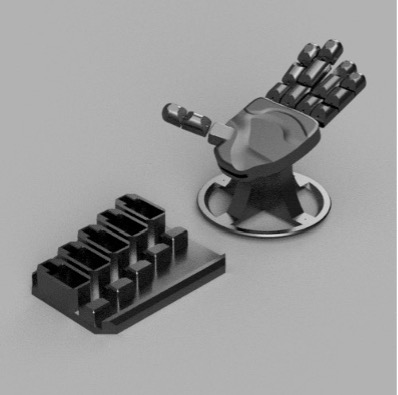
\includegraphics[width=0.8 \linewidth]{Hand_1}}
		\caption{ergonerg}
		\label{fig:Hand_1}		
	\end{center}
\end{figure}
\hfill \break
Das komplexeste Modell ist die Roboterhand, die aus mehreren Elementen besteht, 
darunter die Handfläche sowie die einzelnen Finger, die sich jeweils in drei Glieder 
unterteilen lassen. Der Mechanismus in jedem Finger erfüllt dieselbe Funktion: Durch 
ziehen an der Schnur verkürzt sich ihre Länge, was dazu führt, dass sich der 
jeweilige Finger zusammenzieht. Im Detail betrachtet beschränkt sich der Mechanismus 
des Fingers nicht nur auf das bloße Ziehen an ihm. Der Finger unterteilt in weitere 
Elemente. Er besteht aus drei Gliedern, von denen jedes eine Abschrägung an beiden 
Kanten, die zum nächsten Glied ausgerichtet sind, aufweist. Durch die Verjüngung der 
Kanten, kann beim sogenannten Falten des Fingers dafür gesorgt werden, dass sich der 
Finger auf kleineren Raum zusammenziehen oder auch falten kann. \\
\\
\begin{figure}[H]
	\begin{center}
		\scalebox{1}
		{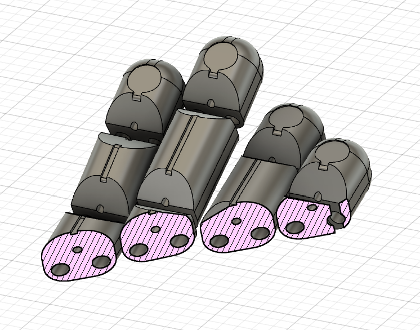
\includegraphics[width=0.8 \linewidth]{Finger_1}}
		\caption{ergonerg}
		\label{fig:Finger_1}		
	\end{center}
\end{figure}
\hfill \break
Wie in dieser Grafik ersichtlich wird hier der Querschnitt aller Finger dargestellt, 
dabei ist es nicht von Relevanz welches der drei Fingerglieder hier genommen wird. 
Alle Glieder, das unterste, das mittlere sowie das oberste Glied haben eine 
gemeinsame Eigenschaft: Durch jeden Finger verlaufen drei Tunnel. Der oberste Tunnel 
hat den Zweck einen Durchgang für die Angelschnur zu schaffen, an dieser wird gezogen 
und bewirkt das Falten des Fingers. \\
\\
\begin{figure}[H]
	\begin{center}
		\scalebox{1}
		{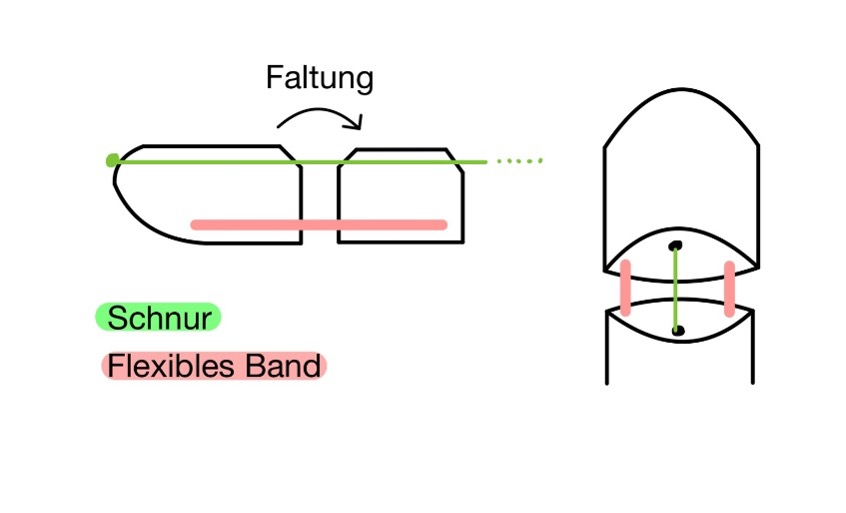
\includegraphics[width=0.8 \linewidth]{Fingerskizze1}}
		\caption{Fingerskizze}
		\label{fig:Fingerskizze1}		
	\end{center}
\end{figure}
\hfill \break
In den beiden unteren Tunneln oder auch Kanälen, 
welche einen ersichtlich größeren Durchmesser von XX mm besitzen verläuft das 
Elastomer, ein elastisches Band. Durch Falten des Fingers, welcher durch Zug an der 
Angelschnur ausgelöst wird, verlängert sich die Strecke auf, die sich das elastische 
Band spannen muss. Dies löst gegengleich zum Zug eine gegenwirkende Spannung aus. 
Anhand der durch das Band entstandenen Zugkraft, behält der Finger seine Position, 
er wird somit gesichert, um weiter in Richtung Zug der Angelschnur zu kippen und 
wiederrum von der Angelschnur, um in Richtung des Bandes zu kippen. Neben der 
Funktion des Rückzuges verbinden die beiden Bänder alle aneinander liegenden 
Fingerglieder sowie auch das unterste Glied mit dem Handflächenelement. Dabei 
spielt auch die Position der Tunnel für das Band eine wesentliche Rolle, denn 
diese verhindern durch ihre Parallele Anordnung, an den unteren äußeren Seiten 
des Gliedes, dass sich die Glieder nach rechts oder links neigen. 
Ebenso befindet sich an dem inneren Teil des Gliedes, welches die Fingerkuppe 
nachstellt, beim Fingerabdruck eine runde Einkerbung sowie ein rechteckiger Kanal. 
Diese Eigenschaft des Modells hält die Option eines optionalen Kraftsensors frei. 
Mit so einem Sensor könnte, bei Integration der Funktion auch die Druckkraft 
gemessen werden. \\
\\
\begin{figure}[H]
	\begin{center}
		\scalebox{1}
		{\includegraphics[width=0.8 \linewidth]{Handfläche_1}}
		\caption{ergonerg}
		\label{fig:Handfläche_1}		
	\end{center}
\end{figure}
\hfill \break
Verbunden sind alle Finger mit dem Element der Handfläche, dieses Element fungiert 
lediglich als Verbindungskomponente zwischen allen Fingern und dem Daumen. 
Im Querschnitt der Handfläche lässt sich erkennen, dass diese von innen einen 
Hohlraum beinhaltet. Dieser Hohlraum hat jeweils einen Kanal zu jedem der Finger, 
sowie Daumen. Dort soll später die Angelschnur durchgeführt werden. Nahe dem 
Handgelenk befindet sich eine große Öffnung, diese ist für alle fünf Schnüre 
gedacht und hat ausreichend Größe für die Schnüre und evtl. auch Kabel für die 
optionalen Kraftsensoren. \\
\\
\begin{figure}[H]
	\begin{center}
		\scalebox{1}
		{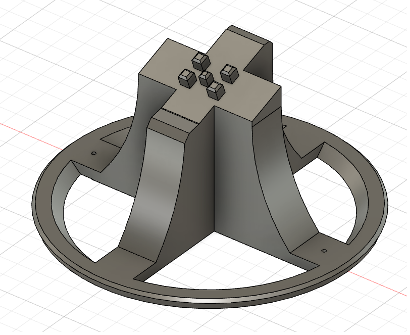
\includegraphics[width=0.8 \linewidth]{Halterung_1}}
		\caption{ergonerg}
		\label{fig:Halterung_1}		
	\end{center}
\end{figure}
\hfill \break
Weiters wurde eine Halterung für die Roboterhand modelliert, diese soll mit 
der Roboterhand verbunden werden. Ihr Zweck ist, die Hand in eine erhöhte und 
leicht geneigte Position zu bringen. Durch das Neigen der Hand werden die fünf 
Angelschnüre bereits in Richtung Antriebsmechanik gerichtet, auch wird bewirkt, 
dass die Hand auf ihrer Höhe nicht unter dem Drehkopf des Servomotors positioniert 
wird. Für die Montage der gesamten Roboterhand auf der Halterung, wird eine 
Aufsteckvorrichtung verwendet. Auf dem Gerüst sind fünf Pins mit einer 
Abschrägung und diese können in die Roboterhand mit Einkerbungen aufgesteckt 
werden. \\
\\
\begin{figure}[H]
	\begin{center}
		\scalebox{1}
		{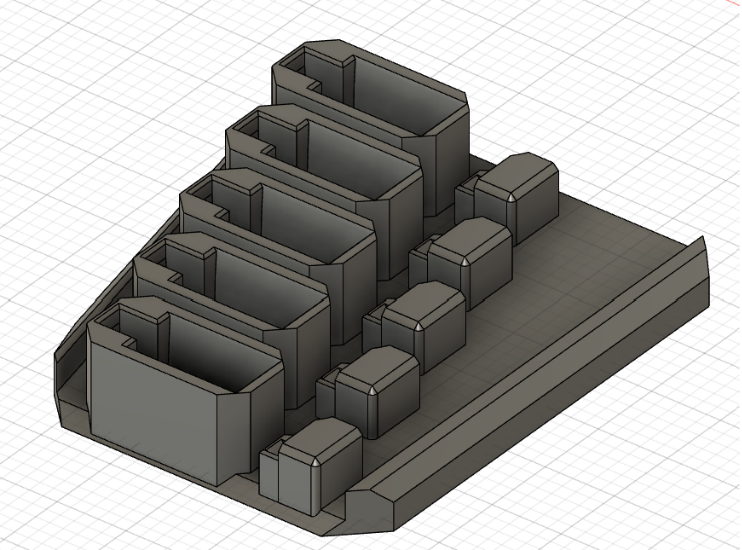
\includegraphics[width=0.8 \linewidth]{Motorblock_1}}
		\caption{ergonerg}
		\label{fig:Motorblock_1}			
	\end{center}
\end{figure}
\hfill \break
Letztlich beinhalt das Modell der Roboterhand ein Element welches hier als 
Motorblock bezeichnet wird, dieses Element trägt diesen Namen da es alle 
für die Antriebsmechanik relevanten Komponenten beinhaltet. \\
Das Modell setzt sich aus einer Grundplatte, der fünf Halterungen für die 
Motoren und jeweils einer passend angeordneten Umlenkung zusammen. \\
Die Halterungen besitzen eine Einkerbung in die der Servomotor eingesteckt 
werden soll, parallel dazu befindet sich eine 90° Umlenkung welche dazu dient, 
dass falls seitlich von unten die Schnur eingeführt wird diese nach oben zum 
Servomotor geführt wird. \\
\\
\textbf{Zusammenbau} \\
\\
Wie bereits erwähnt soll dieser Prototyp mit dem FDM-Druckverfahren gefertigt 
werden. Für den ersten Versuch wurden dabei ausschließlich die Glieder des 
Zeigefingers für den Druck gewählt. \\
Die drei Fingerglieder, wurden mit einem Band und der Schnur befestigt. 
Der erste Versuch, indem ausschließlich der Faltmechanismus und sein 
Verhalten bei Zug am Finger in Erfahrung gebracht werden hat weitlaufende 
Erkenntnisse geliefert. Diese haben zu einem frühzeitigen Abbruch weiterer 
Tests geführt. Die sich dabei erschlossenen Problematiken und Erkenntnisse 
werden im folgenden Kapitel (6.2.2.2 Fazit und Ergebnisse) erläutert. \\
\\

\paragraph{Fazit und Ergebnisse}
\hfill \break
\hfill \break
Der Grundstein für eine bewegliche Hand, welche Finger mit einem 
Faltmechanismus inkludiert wurde mit diesem ersten Entwurf bereits gelegt. 
Dennoch haben sich in der Realität anhand eines einzelnen Versuchs 
entsprechend viele unbekannte Problematiken ergeben die zu einem Verwurf des 
Konzepts geführt haben. \\
\\
Die entstandenen Problematiken:
\begin{itemize}
	\item Da die einzelnen Fingerglieder, bei ihren Verbindungen aneinander 
	aufliegen und sich beim Falten mehr oder weniger aneinander abrollen 
	entsteht zusätzlich mehr Reibung. Dies führt dazu, dass für den Mechanismus 
	zusätzlich mehr Zugkraft benötigt wird.
	\item Demnach ist die Verbindung für immer jeweils zwei Glieder über zwei 
	parallel versetzte Bänder nicht die effizienteste Lösung oder gar die zuverlässigste. 
	Der gewünschte Effekt, dass sich der Finger einklappt, beziehungsweise 
	faltet ist geschaffen, jedoch hat der Finger keine Stabilität. Würde man 
	ihn nach hinten biegen wollen, obwohl er bereits zu 50\% eingefaltet ist, 
	hätte man ein Spiel, mit dem es möglich wäre ihn zu formen. Beim Anhängen 
	einer Last direkt an der Fingerkuppe oder auf das mittlere Fingerglied, 
	müsste somit ausschließlich die Zugschnur dafür sorgen, dass der Finger 
	weiterhin seine Form beibehält. Sinnhafter wäre es somit die Fingerglieder 
	so zu modellieren, dass sich der Finger nicht nach Außen falten oder in 
	diesem Fall besser gesagt biegen lässt, sondern ausschließlich nach Innen. 
	Weiters ist auch bei der Verbindung anzumerken, dass der Finger sich auch 
	nach links oder rechts biegen kann. Diese Funktion ist jedoch nicht 
	erwünscht und muss mechanisch blockiert werden, nur die Verwendung der 
	Bänder ist zu schwach um dies zu verhindern.
	\begin{figure}[H]
		\begin{center}
			\scalebox{1}
			{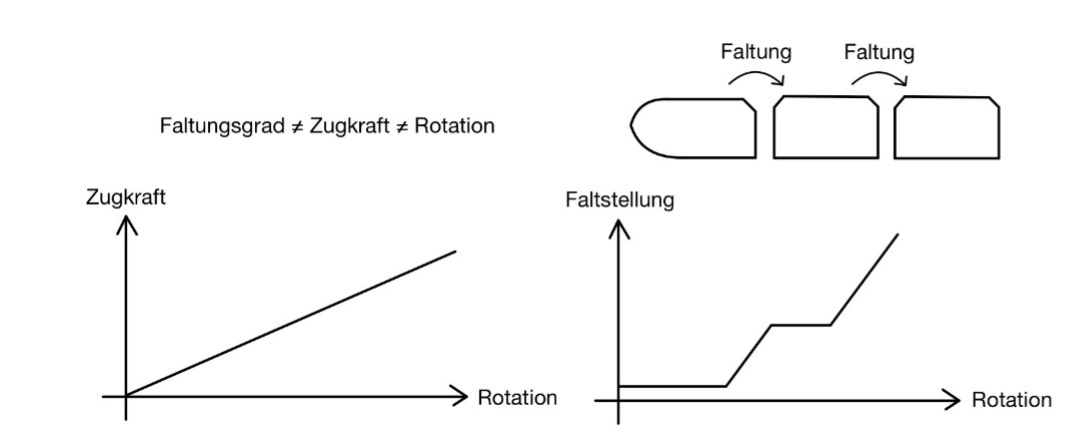
\includegraphics[width=0.8 \linewidth]{Fingerskizze2}}
			\caption{Fingerskizze}
			\label{fig:Fingerskizze2}			
		\end{center}
	\end{figure}
	\hfill \break
	\item Eine Fehlkonstruktion war wie bereits erwähnt die Fläche zwischen 
	beiden Fingern, die zu einem zu mehr Reibung führt aber auch den einzelnen 
	Glieder aufgrund ihrer flachen Fläche und kantigen Fläche nicht ermöglicht 
	sich aneinander abzurollen. Dies führt dazu, dass sich der Finger bei ausreichend 
	Zugkraft einklappt und nicht gleichmäßig abrollt. Wobei dies von großer 
	Bedeutung ist, da somit nicht mit linear ansteigender Zugkraft für eine 
	gleichmäßige Faltung gesorgt werden kann.
	\item Ebenso führt auch der Durchgang, welcher für die Zugschnur ist zu 
	einem Problem. An jedem Ausgang des Tunnels reibt die Schnur stark an den 
	Rändern und dies führt zu mehr Reibung, sowie einem Schaden am Finger.
	Somit muss zusätzlich mehr Kraft angewendet werden.
\end{itemize}

\textbf{Fazit} \\
\\
Wie im Kapitel (6.2.2.2 Realisierung und Zusammenbau) erwähnt wurde aufgrund 
dieser Erkenntnisse der weitere Zusammenbau der Hand vorzeitig beendet und das 
Modell der Hand erstmalig verworfen. \\
Dennoch ist dieser Versuch äußerst lehrreich für die Entwicklung eines weiteren 
Prototypen, denn Reibung, Stabilität und die dadurch benötigte Kraft sind nun 
weitere Einflussfaktoren, auf diese in weiteren Designs mehr geachtet werden 
muss. \\
Auch hat sich gezeigt, dass der Faltmechanismus umsetzbar ist, jedoch ein Konstrukt 
erfordert, welches dem Finger ermöglicht sich in einem gleichmäßigen Verhältnis 
zur Zugkraft zu Falten. \\
\\

\subsubsection{Zweite Testhand (Inmoov)}
\label{chap:Zweite Testhand}
\paragraph{Einführung}
\hfill \break
\hfill \break
Im Versuch der „ersten Testhand“ haben sich zahlreiche Problematiken und 
Erkenntnisse ergeben, demnach erfordert die Weiterentwicklung der Hand, 
die Unterstützung externer Fachkenntnisse.
Nach Recherche im Internet, hat sich ergeben, dass ein französischer 
Bildhauer Gael Levin bereits 2012 für einen damaligen Kunden eine Handprothese 
entworfen hat und damit den Grundstein für sein für sein heutiges Projekt 
InMoov gelegt hat. InMoov ist der erste Open-Source 3D-Druckbare humanoide 
Roboter in 1:1 Größe und ist gedacht für Forschung an Universitäten, in 
Laboratorien und auch für private Zwecke. \\
Ein großer Vorteil des Projekts ist es, das bereits viele Erkenntnisse und 
Wissen in dieses eingeflossen sind. Ziel ist es dieses 3D druckbare Hand 
selbst zu realisieren, je nach Anforderung zu modifizieren und anhand dessen 
eine weitere Versuchshand zu schaffen. \\
\\

\paragraph{Mechanismus}
\label{par:Mechanismus_zweite_Hand}
\hfill \break
\hfill \break
Der Mechanismus der zweiten Versuchshand \"InMoov\" ist äußerst umfangreich und weist meist bessere Lösungen für Features der ersten Versuchshand aus \autoref{chap:Erste Testhand} auf. \\
\\
\begin{figure}[H]
	\begin{center}
		\scalebox{1}
		{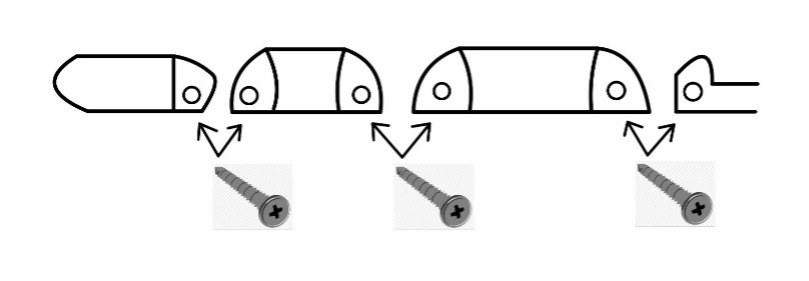
\includegraphics[width=0.8 \linewidth]{Fingerskizze3}}
		\caption{Fingerskizze}
		\label{fig:Fingerskizze3}			
	\end{center}
\end{figure}
\hfill \break
Die Problematik, dass wie beim vorherigen Modell die beiden Glieder aneinander reiben und sich nicht parallel zur Zugkraft kontinuierlich umrollen ist hier nicht vorhanden, da die Konstruktion von Grund auf andere Eigenschaften aufweist. 
Denn die jeweiligen Glieder werden hier nicht mit Bändern verbunden, sondern mit einer Schraube, welche die beiden Glieder, die ineinander gehen verbinden. Durch diese Verbindung sind die Finger zu einem stabil – können nicht nach links und 
rechts kippen und sich ausschließlich vom ausgestreckten Zustand nach innen Falten. Auch wird mechanisch ein Falten in die andere Richtung, verhindert. \\
\\
\begin{figure}[H]
	\begin{center}
		\scalebox{1}
		{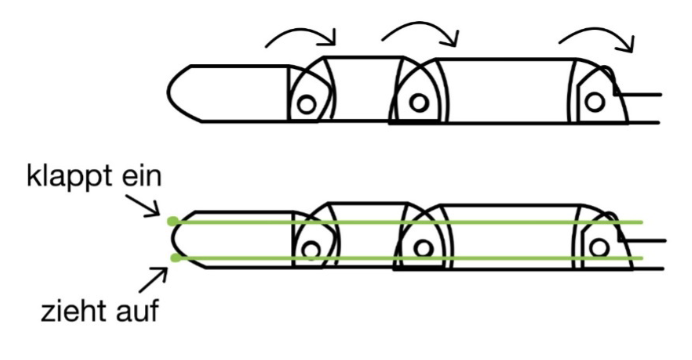
\includegraphics[width=0.8 \linewidth]{Fingerskizze4}}
		\caption{Fingerskizze}
		\label{fig:Fingerskizze4}			
	\end{center}
\end{figure}
\hfill \break
Am tatsächlichen Faltmechanismus hat sich bis auf einer Anpassung am Elastomer nicht viel geändert, denn der Rückzug erfolgt nicht mehr traditionell per elastischem Band. Diese Umsetzung des Faltmechanismus ist jedoch von großer Bedeutung, dar 
nur der Rückzug sowie der Faltung von ein und demselben Motor ausgelöst wird. Im Detail funktioniert der Mechanismus wie mit Hilfe der Grafik ersichtlich wie folgt: Am Servomotor wird eine runde Vorrichtung montiert, diese hat an der Außenkante 
eine beidseitige Verjüngung, an dieser soll die Schnur entlanglaufen. Nun verlaufen beide Schnüre, die für den Ein- sowie Auszug verantwortlichen Schnüre, jeweils auf einer Seite, an dieser Runden Vorrichtung und sind an dem Ende dieser montiert. 
Dreht sich nun der Motor um 90\textdegree gibt er mehr der Schnur(1) her und verkürzt die Schnur(2). Bei diesem Vorgang müssen jedoch beide Schnüre so gespannt sein, dass keine der beiden nachgibt und sich bei Bewegung des Motors lockert. \\
\\
Das Modell der Handfläche, an dem alle Finger und weitere Komponenten zentral zusammenkommen setzt sich selbst aus insgesamt vier tatsächlichen Elementen zusammen und zwei Hilfselementen. \\
Das Hauptelement ist in dem Fall wie in der Grafik ersichtlich (1), dies ist das Größte und Zentrale Element, durch dieses Element verlaufen 15 Kanäle, die mittleren fünf dienen optionaler Sensorik. Die oberen fünf Kanäle sind für die Schnüre, 
welche dem Einfalten dienen, die oberen dienen der Schnüre für den Rückzug. \\
Um die Hand noch dynamischer zu gestalten besitzen der Ringfinger sowie der Kleinefinger ein zusätzliches Element (2) sowie (3), welches sich bei Zug auf wenige Grad mit faltet. Der Daumen hat eine ähnliche Funktion, Element (4) in der Grafik. \\
Als Hilfselement werden hier die Stifte (5) und (6) welche zur Verbindung zwischen Element (1) sowie den weiteren Elementen dienen. \\
\\
Ein ebenso neuer und optionaler Mechanismus ist die des Handgelenks, dieser ermöglicht es der Hand um ihre eigene Achse zu rotieren. Umgesetzt wird dies mit einem Servomotor, welcher mit einer Übersetzung anhand zweier Zahnräder die Hand rotiert. \\
\\
Montiert wird dieser Handgelenksmechanismus auf ein Unterarmkonstrukt, dieses besteht aus mehreren einzelnen Teilen um den Druck auf mit einem kleinen Drucker zu ermöglichen. Grundsätzlich sind alle Modelle des Projekts \"InMoov\" auf einem Drucker 
mit einer Druckfläche von $12x12x12cm$ ausgelegt. \\
\\
\begin{figure}[H]
	\begin{center}
		\scalebox{1.2}
		{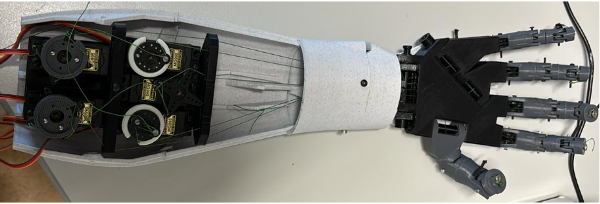
\includegraphics[width=0.8 \linewidth]{Roboterhand_Version2}}
		\caption{Roboterhand zweite Version}
		\label{fig:Roboterhand_Version2}			
	\end{center}
\end{figure}
\hfill \break
Im Unterarm befindet sich an der Innenseite eine Umlenkung, die die Schnüre über den Rotationsmechanismus des Handgelenks lenkt. Dies verhindert vor allem eine Reibung zwischen der Schnüre und dem Servomotor für das Handgelenk, welcher in der 
idealen Strecke zwischen Schnur und Zielmotor steht. \\
\\
Weiters werden daraufhin die Schnüre zum Motorblock der Antriebsmechanik für den Faltmechanismus der Finger geführt. In diesem Block befinden sich fünf Motoren, für die Finger.
Dort wird der bereits beschriebene Mechanismus der beiden Schnüre umgesetzt. \\
\\
Wurde ein Modell in einer CAD-Software wie beispielsweise Fusion 360 entworfen und soll nun in ein reales greifbares Objekt umgewandelt werden, so benötigt man eine sogenannte Slicer-Software. Die Bezeichnung \"Slicer\" stammt dabei vom englischen 
Wort Slice (engl.) und bedeutet so viel wie Scheibe. Dies stammt der Tatsache ab, dass diese Software das 3D-Modell in einzelne Scheiben mit einer Sichthöhe geringer als 1mm teilt, denn wie bereits in \autoref{par:Fertigung und CAD} erklärt, geht das 3D-Druck Verfahren 
FDM so beim Schaffen eines realen Objekts vor. \\
Gewählt wird die Open-Source Software Ultimaker Cura, in der Version 5.6.0, in diesem kann man zahlreiche Optionen treffen: Die Sichthöhe der einzelnen Scheiben, in Fachsprache "Layers", die Druckgeschwindigkeit, die Füllungsdichte, ob Stützstrukturen für den 
Druck vorhanden sein sollen oder nicht. Durch das Regeln dieser Optionen wird die Druckqualität beeinflusst, druckt der Drucker zu schnell so leidet die Qualität und es können Fehler im Druck auftauchen, ist die Schichthöhe zu hoch ist der Druck 
äußerst ungenau und weist eine unschöne Textur an seiner Oberfläche auf. \\
Auch können Faktoren, wie die Drucktemperatur oder das Filament gewählt werden. Je nach Filament gibt es bereits im Vorhinein konfigurierte Optionen. \\
\\
Sind nun alle gewünschten Werte angepasst, kann „gesliced“ werden dabei wird nun von der Software das Objekt in einzelne Scheiben geteilt und ein g-code File erstellt, welches dem Drucker daraufhin Anweisungen gibt. \\
\\
Ein Druck dauert in der Regel mehrere Stunden, dies variiert jedoch je nach Drucker – neuere schaffen das selbe Ergebnis in 20\% der eigentlichen Druckzeit. \\
Nach einiger Zeit ist der Druck fertig und kann von der Druckplatte gelöst werden, vorhandene Stützstrukturen können im Bestfall einfach vom Druck gelöst werden. \\
\\
Für den Zusammenbau der InMoov Hand werden neben dem Druck auch weitere Elemente benötigt, die nicht aus dem 3D-Drucker stammen. 
Als Auflistung die zusätzlich benötigten Komponenten:
\begin{itemize}
	\item 16 Stück M3x20mm Schrauben
	\item 16 Stück M3-Mutter
	\item Superkleber
	\item Angelschnur: 3 Meter
\end{itemize}

\paragraph{Fazit und Ergebnisse}
\hfill \break
\hfill \break
Der Versuchsaufbau hat nur kurzfristig und teilweise funktioniert. Für einen kurzen Moment konnten alle Finger, sowie der Daumen geöffnet und geschlossen werden. Der Faltmechanismus hat sich zwar bewiesen, jedoch mit einigen Unstimmigkeiten. \\
Während dem Testen sind zwei Punkte besonders auffällig gewesen: Zu einem die Stabilität mit und ohne Belastung, sowie die Spannung der jeweils beiden Schnüre. Unter die Stabilität fallen in diesem Fall, das gesamte Gerüst vom einzelnen Finger 
bis zum Motorblock, die Antriebsmechanik und ihre Halterung für die Umwicklung. Sowie die Schnüre, welche einige Probleme und demnach auch Schäden verursacht haben. \\
\\
\textbf{Problematik-1: "Unstimmigkeiten bei dem Umwickeln der jeweils beiden Schnüre"} \\
Wie in \autoref{par:Mechanismus_zweite_Hand} erläutert, sollen sich beide Schnüre um eine runde Halterung wickeln und dabei je nach Drehung den verbundenen Finger ein -oder auffalten. Damit dieser Mechanismus funktioniert müssen beide Schnüre 
ständig unter Spannung stehen, da sonst die Gegenwirkung des Systems nicht vorhanden ist und der Finger Überklappen kann. \\
Es gab mehrere Lösungsversuche, zu einem den Servomotor in 5° Schritten von 0 bis 180\textdegree Grad approximieren und dabei während jedem Schritt die Schnüre nach zu spannen, jedoch blieb auch dies erfolglos. \\
\\
\textbf{Problematik-2: "Instabilität der Halterungen auf dem Motor"} \\
Die Angelschnur hat neben ihren Vorteilen auch einen trivialen Nachteil, denn sie ist sehr dünn und daraus folglich unter Spannung äußerst schneidend. Stand die Schnur unter zu hoher Spannung hat dies dazu geführt, dass diese sich 
selbst aufgrund der zu hohen Reibung durch die Halterung am Motor geschnitten hat und ihn dabei meist auch horizontal zerteilt. Nach Erkenntnis dieses Problems gab es drei grundlegende Lösungsversuch:

\begin{itemize}
	\item \textbf{Lösungsversuch 1:} \\
	Hier wurde versucht das gedruckte Objekt selbst härter und dicker zu drucken. Umgesetzt wurde das durch Erhöhen der Fülldichte von 25\% auf 65\%, dadurch ist das innere Modell von Innen dichter ist. Weiters wurde auch die Wandstärke 
	und -dicke erhöht. \\
	Das Ergebnis war ernüchternd, bereits nach neuem Anspannen führte es bereits wieder zum selben Problem und die Halterung hielt nicht stand.
	\item \textbf{Lösungsversuch 2:} \\
	Nach genauerem Hinblick wurde klar, es liegt am Druckverfahren, denn wie bereits erklärt druckt der Drucker in einzelnen Schichten. Das Problem: Die Schnur liegt parallel zu den einzelnen Schichten und genau zwischen diesen Schichten 
	liegen die Schwachpunkte des Modells. Somit wurde die Entscheidung getroffen das Modell so zu drucken, dass die Schnur und die einzelnen Schichten nicht parallel zueinander liegen, bewirkt wurde dies indem die Halterung in einem 45\textdegree 
	Winkel gedruckt wurde.
\end{itemize}
\hfill \break
Der zweite Lösungsversuch ist somit erfolgreich und die Schnur schneidet oder halbiert nicht mehr die Halterung. Jedoch nicht perfekt, denn die Schnur reibt an der gerippelten Oberfläche der Halterung. In diesem Fall muss ein anderes Material als 
PLA und damit auch ein anderes 3D-Druck Verfahren verwendet werden. Ergeben hat sich der SLS (engl. Selective Laser Sintering). Dies ist ebenso eine additive Fertigungstechnologie, dabei verschmilzt ein Laser selektiv Pulverpartikel und das 
schichtweise um daraus dann das gewünschte 3D-Objekt zu fertigen. Finalerweise entstanden dann für das Projekt Halterungen aus dem Material Nylon mit Glasfaserverstärkung. %\footnote{\url{https://sls3d.de/wissen/was-ist-selektives-lasersintern/\#:\~:text=SLS\%20\%E2%80%93%20engl.,(3D\%2DDruck)\%20aufzubauen}, (Stand: 24.02.2024)} \\
\\
\textbf{Problematik-3:} \\
Zwar sind Angelschnüre sehr stabil und stark, tendieren jedoch unter ständiger Reibung trotz ihrer acht fachen Flechtung mit der Zeit zu reißen. Die Strecke von Fingerkuppe, bis zum Motor beträgt dabei je nach Finger zwischen 20-30cm, 
auf dieser Strecke reibt sich die Schnur an mehreren Stellen des Modells auf. Da dieses Problem erst mit der Zeit auftritt und somit mit der Hand dennoch ausgiebig getestet werden kann bis zum nächsten Riss wurde dieses Problem im Versuchsaufbau der 
zweiten Hand noch nicht behandelt. \\
\\
\textbf{Problematik-4: } \\
Ein weiteres Problem ist die Befestigung der Schnur am Fingerende, der Fingerkuppe. Diese hat zwei Bohrungen bzw. Löcher, zwischen diesen werden beide Schnüre befestigt. Das Problem, da diese Schnüre so klein sind und dauerhaft 
unter Spannung stehen reißt die Fläche zwischen den Löchern meist ein und die Schnüre können nicht mehr befestigt werden. \\
\\
Das Modell löst einige Probleme und schafft neue Ansätze. Der Faltmechanismus wurde grundlegend erweitert, der Rückzug wird nun nicht mehr per Elastomer, sondern mit einer zweiten Schnur bewirkt.
Die einzelnen Fingerglieder, sind tatsächlich mechanisch durch eine Schraube miteinander verbunden. \\
All dies führt zu präziseren und genaueren Bewegungen, der Faltmechanismus erfolgt annähernd linear zur Zugkraft. Trotzdem hat sich herausgestellt, wie brüchig das Modell ist, besonders an den Fingern. Reibung ist weiterhin ein großes Thema und 
wird durch die zweite Schnur im Faltmechanismus noch trivialer. \\
Ziel ist es im dritten Versuchsmodell die Problematik mit der Reibung zu verringern und daraus folglich auch ein stabileres Modell zu ermöglichen.\\
\\

\subsubsection{Dritte Testhand (Projekt-Silikonhand)}
\paragraph{Das Konzept}
\hfill \break
\hfill \break
Nachdem die vorherigen Versuche erwiesen, haben welche Problematiken sich aus einem festen Modell aus PLA ergeben, stand ein großes Umdenken im Raum. Auf Vorschlag einer Betreuungskraft stellte sich heraus, dass das Modell elastischer sein muss und 
ein hartes Material nicht immer die Beste Lösung ist. Der Vorschlag war Silikon in das Modell der Hand zu integrieren, ein ähnliches Projekt habe so bereits eine Hand realisiert. Ähnlich wie bei dem Modell aus \autoref{chap:Erste Testhand} bestanden 
dort die einzelnen Glieder aus einzelnen Teilen, zwar aus Silikon, waren jedoch auch per Elastomer verbunden. Die Handfläche bestand bei dem Modell aus dem Vorschlag dennoch aus harten Kunststoff. \\
\\
Für das Projekt "Bionic-Hand" ergab sich eine neue Ebene und Vielfalt der Möglichkeiten. Die neue Idee ist es die gesamte Hand vollständig aus Silikon zu entwickeln und somit Problemen wie der Reibung und Brüchen unter starker Last aus dem 
Weg zu gehen. \\
\\
Genauer lässt sich das neue Konzept wie folgt beschreiben: Die gesamte Hand besteht aus dem Material Silikon, seien es die einzelnen Finger, der Daumen und die Handfläche. Daraus ergeben sich mehrere Vorteile. Zu einem ein Grip (engl.), aufgrund des 
Silikons hat die Hand beim Greifen mehr Griff und Objekte können gehalten werden, ohne aus der Hand zu rutschen. Der nächste Vorteil ist, dass die Hand anpassbarer wird und sich aufgrund ihrer elastischen Struktur genau um das Objekt stülpen kann, 
dies ist eine große Verbesserung im Vergleich zu der festen Hand aus hartem Kunststoff. \\
Ein Hand aus Silikon springt von selbst wieder in ihre Ursprungsposition zurück, dies liegt an den Eigenschaften des Materials, dadurch wird sich ein externer Elastomer erspart, der Rückzug erledigt sich von selbst. Die Fingerglieder der Hand sollen 
ähnlich wie bei den vorherigen Modellen eine Verjüngung zueinander haben und durch Zug an der Schnur der Finger sich Falten. Reibung dürfte nach Überlegungen nicht mehr existieren, da die Schnur bei Bewegt das Material eher bewegt und nicht wirklich 
reibt. Befestigt wird dies dann an einer Vorrichtung am Handgelenk. \\
\\

\paragraph{Gussform}
\label{par:Gussform}
\hfill \break
\hfill \break
Eine Herausforderung von diesem Versuchsmodell ist das Verfahren des Silikongusses, um das Verfahren des Silikon gießen zu verstehen wird eine Gussform in der CAD-Software entworfen. \\
\\
Als Testobjekt wurde ein einfacher Finger, welcher einen Faltmechanismus ermöglicht entworfen. \\
\\
\begin{figure}[H]
	\begin{center}
		\scalebox{1.2}
		{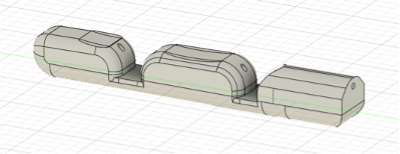
\includegraphics[width=0.8 \linewidth]{Silikon_Testfinger1}}
		\caption{Silikon-Testfinger}
		\label{fig:Silikon_Testfinger1}			
	\end{center}
\end{figure}
\hfill \break
Im oberen Teil des Fingers verläuft durch jedes einzelne Glied ein Kanal, für die Zugschnur, die Verbindungen zwischen den einzelnen Gliedern wird durch eine Fläche geschaffen. Bei Zug faltet sich dann der Finger an den dünneren Punkten des Objekts. \\
\\
\begin{figure}[H]
	\begin{center}
		\scalebox{1.2}
		{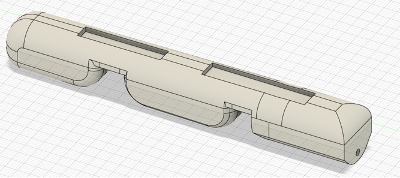
\includegraphics[width=0.8 \linewidth]{Silikon_Testfinger2}}
		\caption{Silikon-Testfinger}
		\label{fig:Silikon_Testfinger2}			
	\end{center}
\end{figure}
\hfill \break
Um diese Fläche optional nochmals im Nachhinein zu verdicken und dadurch zu beeinflussen, wie stark der Rückzug ist wurden zwei Einkerbungen in das Modell des Fingers implementiert. Durch das Aufgießen mit Silikon dieser rechteckigen Einkerbungen 
an den Biegungspunkten, kann dies bewirkt werden. \\
\\
Der ganze Finger wird in eine Gussform gegossen, diese besteht aus zwei Teilen um den Finger leicht aus der Form lösen zu können, ohne dabei die beiden Objekte zu beschädigen. \\
Verbunden sind beide Teile der Form mit einem Steckmechanismus, wie in der Grafik (x.x.x) ersichtlich. Am oberen Teil der Gussform befindet sich ein Loch in dieses wird das flüssige Silikon später gegossen, das Loch wurde extra groß 
dimensioniert damit gleichzeitig auch die Luft im Innenraum entweichen kann. \\
\\
\begin{figure}[H]
	\begin{center}
		\scalebox{1.2}
		{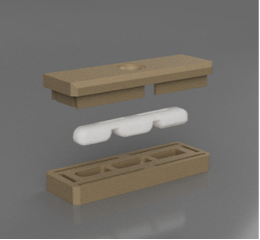
\includegraphics[width=0.8 \linewidth]{Silikon_Testfinger_Gussform}}
		\caption{Silikon-Testfinger-Gussform}
		\label{fig:Silikon_Testfinger_Gussform}			
	\end{center}
\end{figure}
\hfill \break
\textcolor{red}{Quelle: https://silikon-profis.de/2-Komponenten-Massen\#:\~:text=2\%2D\%20Komponenten\%20Silikonkautschuke\%20vulkanisieren\%20bei,anspruchsvolle\%20Profi\%2DAbformungen\%20und\%20Gie\%C3\%9Fverfahren} \\
\\
Das hier verwendete flüssig Silikon besteht aus zwei Komponenten welche als Teil A und Teil B bezeichnet werden. Teil A ist die Hauptkomponente des Silikons und Teil B ist die Härtekomponente, zusammen vermischt führt dies zu einem festen elastischen 
Material. \\
\\
Das Ergebnis nach dem ersten Guss: Während dem Entwurf des Gussform wurde nicht daran gedacht, dass das Loch für den Einguss auf derselben Höhe wie die höchste Fläche oder Decke des Innenraums sein muss. Durch diesen Fehler hat sich ab dieser Höhe 
ein Luftraum gebildet, welcher nicht mit Silikon gefüllt wurde. \\
\\
\textbf{Verbesserung:} \\
\\
\begin{figure}[H]
	\begin{center}
		\scalebox{1.2}
		{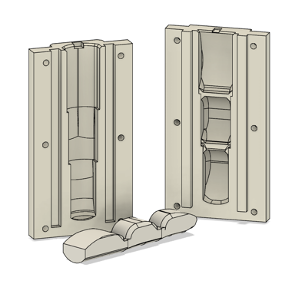
\includegraphics[width=0.8 \linewidth]{Silikon_Testfinger_Verbesserung}}
		\caption{Silikon-Testfinger-Verbesserung}
		\label{fig:Silikon_Testfinger_Verbesserung}			
	\end{center}
\end{figure}
\hfill \break
Dies wurde durch eine Form, in der der Finger aufrechtstehend gegossen werden soll verbessert. Das Loch ist somit am Anfang des Fingers und die Luft kann vollständig entweichen. Eine kleine Anpassung ist, dass neben dem Steckmechanismus auch eine 
Verschraubungsmöglichkeit geschaffen wurde um die beiden Teile der Gussform stärker aneinander zu pressen, dies verhindert das Austreten von Silikon während dem Guss. \\
Gezeigt hat sich nach dem Guss, dass das fertige Objekt aus Silikon, sich auch in andere Richtungen biegen lässt als ausschließlich in die Faltrichtung. Um alle anderen Richtung außer die gewünschte zu verhindern, benötigt der Finger einen 
Stabilisator von Innen, ähnlich wie der Finger des Menschen, welche einen Knochen hat. \\
\\

\paragraph{Gelenke}
\hfill \break
\hfill \break
Um zu verhindern, dass sich der Finger nach links, rechts, oder nach hinten biegt also nicht in die Richtung, in die er sich Falten soll wird im Inneren des Fingers etwas benötigt, dass nur das Biegen in die Faltrichtung erlaubt. Somit ein 
mechanisches Gelenk welches durch den gesamten Finger geht. \\
\\
\begin{figure}[H]
	\begin{center}
		\scalebox{1.2}
		{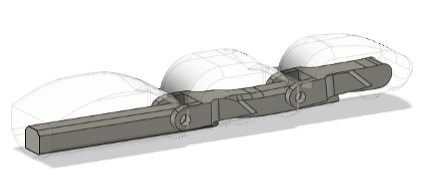
\includegraphics[width=0.8 \linewidth]{Gelenke1}}
		\caption{Fingergelenke}
		\label{fig:Gelenke1}			
	\end{center}
\end{figure}
\begin{figure}[H]
	\begin{center}
		\scalebox{1.2}
		{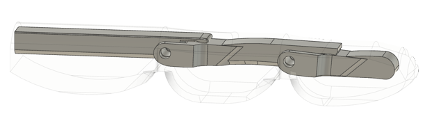
\includegraphics[width=0.8 \linewidth]{Gelenke2}}
		\caption{Fingergelenke}
		\label{fig:Gelenke2}			
	\end{center}
\end{figure}
\hfill \break
Das Gelenk besteht aus drei Komponenten, verbunden sind diese durch eine Schraube, exakt an dem Punkt an dem sich der Finger beim Falten biegt. Durch eine mechanische Blockade kann sich das Gelenk ausschließlich in Faltrichtung falten. \\
Mit einer Erweiterung wird das gesamte Modell in der Gussform befestigt und positioniert, nach dem Guss findet sich dann das Gelenk eingegossen im Finger. \\
\\
\textbf{Ergebnis:} \\
\\
Während des Gusses ist Silikon ausgetreten, obwohl bereits im Vorhinein vorgesorgt wurde, damit dies nicht passiert – wie die Verschraub Möglichkeiten, mit denen beide Teile aneinander gepresst werden sollen oder die Steckvorrichtung. 
Gelöst konnte dies mit Klebebändern, die zum Abdichten verwendet wurden. \\
Trotz der Komplikationen, hat sich der Versuch als erfolgreich herausgestellt, denn der Finger funktioniert in Zusammenspiel mit dem Gelenk wie erwartet. \\
\\
\begin{figure}[H]
	\begin{center}
		\scalebox{1.2}
		{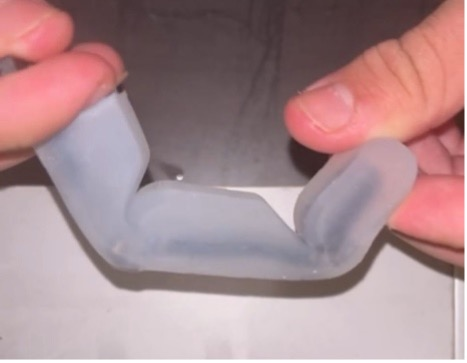
\includegraphics[width=0.8 \linewidth]{Gelenke_real}}
		\caption{Gelenke in echt}
		\label{fig:Gelenke_real}			
	\end{center}
\end{figure}
\hfill \break

\paragraph{Entwurf einer neuen Gussform}
\hfill \break
\hfill \break
Nachdem sich gezeigt hat, dass ein einzelner Finger umsetzbar ist der nächste Schritt eine gesamte Hand zu entwerfen. Für diese wird somit ein vollständiges Gelenksgerüst für die gesamte Hand benötigt, ein Modell einer Hand sowie eine dafür entworfene 
Gussform. \\
\\
Das Modell der Hand – Grundsätzlich ist Ziel die gesamte Hand aus Silikon zu verwirklich und diese aus Silikon zu gießen. Der Faltmechanismus funktioniert dabei wie in Kapitel (6.2.4.2 Finger), mit der zusätzlichen Eigenschaft, dass die Finger früher 
in der Handfläche beginnen, damit sich diese besser um das gewünschte Objekt "Falten" kann. \\
\\
\begin{figure}[H]
	\begin{center}
		\scalebox{1.2}
		{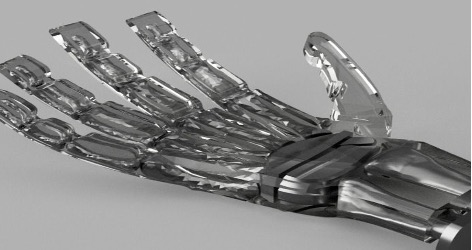
\includegraphics[width=0.8 \linewidth]{Silikonhand_3Dmodell}}
		\caption{3D-Modell Silikonhand}
		\label{fig:Silikonhand_3Dmodell}			
	\end{center}
\end{figure}
\begin{figure}[H]
	\begin{center}
		\scalebox{1.2}
		{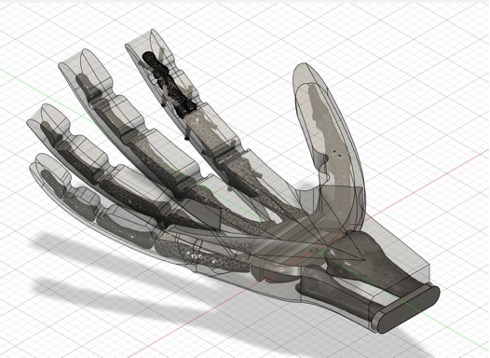
\includegraphics[width=0.8 \linewidth]{Silikonhand_3Dmodell2}}
		\caption{3D-Modell Silikonhand}
		\label{fig:Silikonhand_3Dmodell2}			
	\end{center}
\end{figure}
\hfill \break
Ohne nun bereits auf das Gerüst einzugehen ist in dieser Grafik zu sehen, dass die Handfläche zwischen den Fingern kein Material hat. Dies schafft auch die optionale Möglichkeit die Finger mit einem weiteren Mechanismus seitlich zu bewegen. \\
In der Grafik ist ebenso die sich von den anderen Fingern unterscheidende Anordnung des Daumens, dieser liegt seitlich und soll beim Falten sich ähnlich wie der echte Daumen des Menschen verhalten.
Das Gerüst hat dabei eine triviale Neuerung, denn es wurde sich an den tatsächlichen Knochen eines Menschen orientiert, damit soll für mehr Ähnlichkeit zur Anatomie der menschlichen Hand gesorgt werden. \\
\\
\begin{figure}[H]
	\begin{center}
		\scalebox{1.2}
		{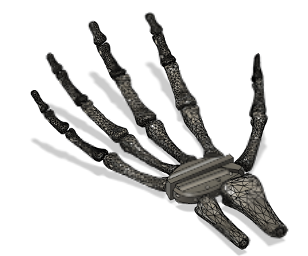
\includegraphics[width=0.8 \linewidth]{Skelett1}}
		\caption{Skelett}
		\label{fig:Skelett1}			
	\end{center}
\end{figure}
\begin{figure}[H]
	\begin{center}
		\scalebox{1.2}
		{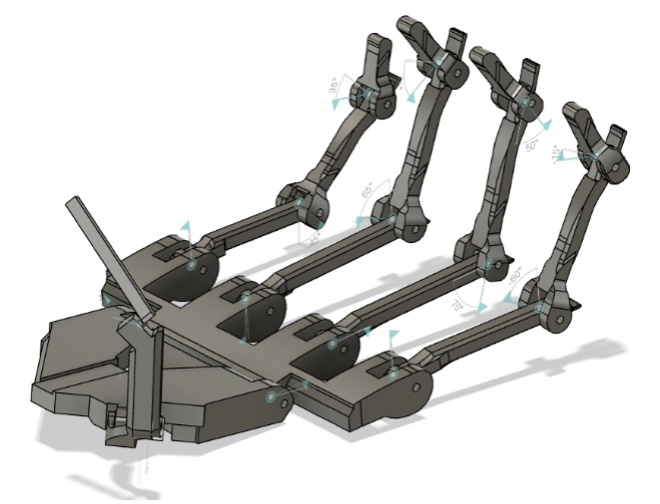
\includegraphics[width=0.8 \linewidth]{Skelett2}}
		\caption{Skelett}
		\label{fig:Skelett2}			
	\end{center}
\end{figure}
\hfill \break
Im Unterschied zu einer vorherigen Version des Gerüsts, ist zu erkennen, welche Vorteile die neue gegenüber ihr hat. Zu einem ist diese viel flexibler und hat keine große und starre Handwurzel. 
Ein weiter Unterschied ist die Verbindung der einzelnen Knochen in jedem Finger. Anders wie bei der alten Version werden hier keine Schrauben zu der Verbindung einzelner Gelenksteile, sondern Gummikordeln verwendet. \\
\\
\begin{figure}[H]
	\begin{center}
		\scalebox{1.2}
		{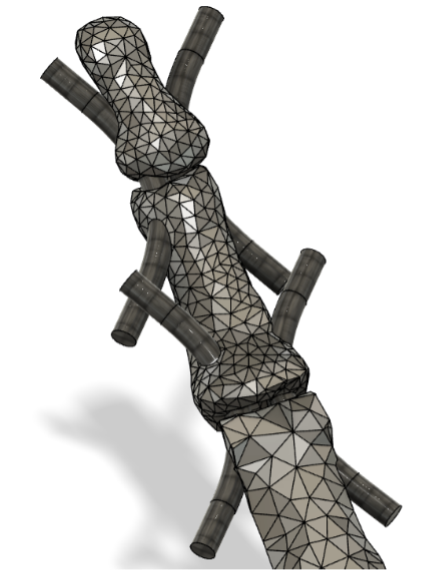
\includegraphics[width=0.8 \linewidth]{Fingerglieder}}
		\caption{Fingerglieder}
		\label{fig:Fingerglieder}			
	\end{center}
\end{figure}
\hfill \break
Diese neue Form der Verbindung war notwendig um die einzelnen Elemente der Knochen platzsparend und effektiv zu verbinden. Zwar wurde kurzzeitig eine Verbindung anhand einer Schraube getestet, dies zeigte jedoch, dass das mit der Größe der Knochen 
und dem Raum im Finger nicht umsetzbar wäre. Zwar blockiert dieser Mechanismus nicht Bewegungen in alle anderen Richtungen außer die Faltrichtung, schafft jedoch mehr Flexibilität für den Finger – dennoch wurde jeder Finger so modelliert und an den 
Krümmungsstellen so verstärkt, dass er sich hauptsächlich in die Faltrichtung biegt. \\
\\

\paragraph{Gussform und Gussversuch}
\hfill \break
\hfill \break
Für den Guss der gesamten Hand wird ähnlich wie bei dem Finger aus Versuch von Kapitel (x.x.x), eine Gussform benötigt, diese Gussform hat jedoch ein größeres Spektrum an Anforderungen. Mitunter muss berücksichtigt werden, dass das "Skelet" auch 
bekannt als das Gelenksgerüst präzise in der Mitte eines Fingers platziert werden muss. \\
\\
\begin{figure}[H]
	\begin{center}
		\scalebox{1.2}
		{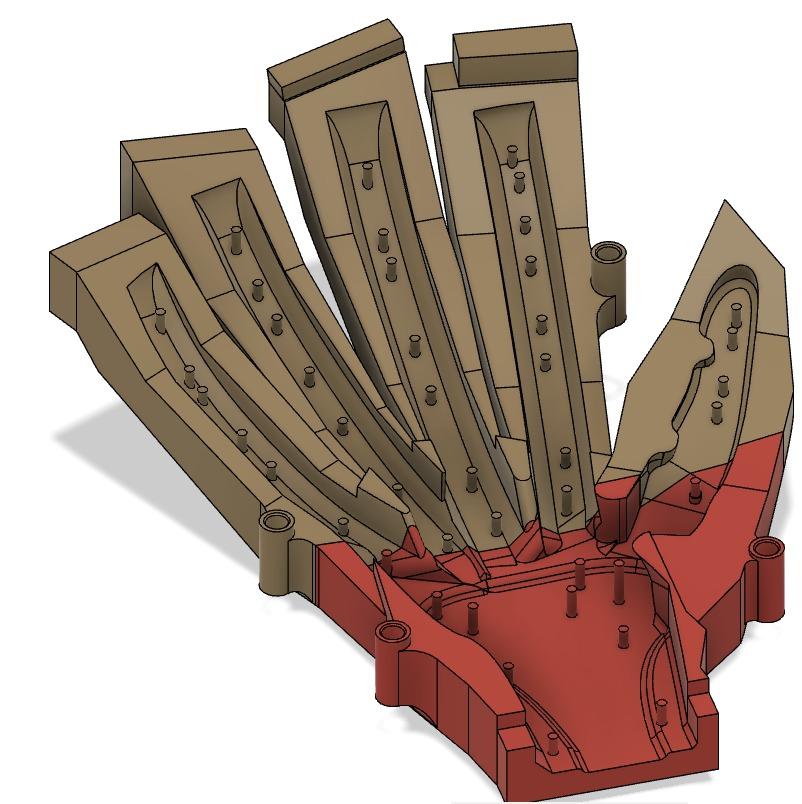
\includegraphics[width=0.8 \linewidth]{Gussform1}}
		\caption{Gussform}
		\label{fig:Gussform1}			
	\end{center}
\end{figure}
\begin{figure}[H]
	\begin{center}
		\scalebox{1.2}
		{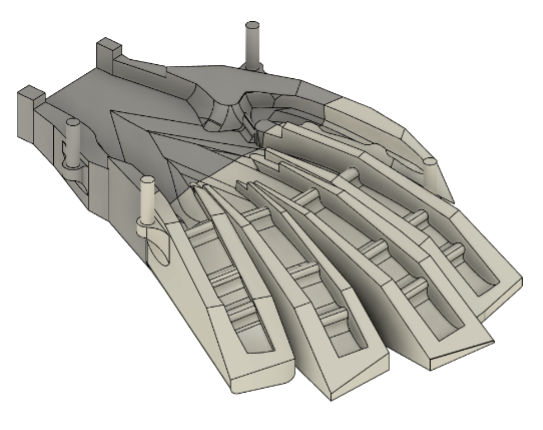
\includegraphics[width=0.8 \linewidth]{Gussform2}}
		\caption{Gussform}
		\label{fig:Gussform2}			
	\end{center}
\end{figure}
\hfill \break
Zu sehen sind in den beiden Grafiken, vier Teile der Gussform, dies ist darauf zurückzuführen, dass die Druckfläche des Druckers sonst überschritten werden würde. Daher muss jeweils der untere und der obere Teil der Form halbiert werden. Zu der 
unteren Hälfte der Gussform in der linken Grafik gehört das rote und braune Element und zu der oberen gehören wie in der rechten Grafik sichtbar das beige und graue Element. Befestigt werden die beiden Teile jeweils mit vier Stiften in Form einer 
Steckvorrichtung. Sichtbar ist ebenso zwischen dem unteren und dem oberen Element der Gussform eine weitere Steckvorrichtung, durch diese werden beide Hälften der Form verbunden. \\
\\
\begin{figure}[H]
	\begin{center}
		\scalebox{1.2}
		{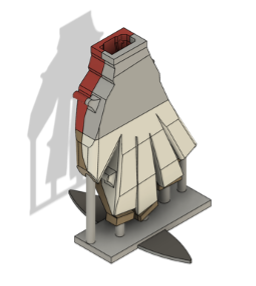
\includegraphics[width=0.8 \linewidth]{Gussform3}}
		\caption{Gussform}
		\label{fig:Gussform3}			
	\end{center}
\end{figure}
\hfill \break
Wie in dieser Veranschaulichung ersichtlich wird in aufrechtem Zustand der Gussform das Silikon in das obere Loch eingegossen. Wie in \autoref{par:Gussform} an einem Versuch zu sehen ist, ist es von großer Bedeutung, dass das Eingussloch an der höchsten 
Stelle des Innenraums liegt. Um sicherzustellen, dass die Hand stets aufrecht bleibt und während dem Härteprozess des Silikons nicht gesichert in ihrer Position bleibt wurde eine Halterung entworfen, auf diese Kann die Form gesteckt werden. Das Loch 
wurde möglichst groß modelliert, damit die im Innenraum verbleibende Luft der Gussform ausreichend entweichen kann. \\
\\
\textbf{Der Guss:} \\
\\
Der Gussprozess ist nicht einwandfrei verlaufen, mitunter lag dies hauptsächlich an den Lücken zwischen den einzelnen Elementen. Aufgrund des FDM-Druckverfahren sind zwischen den einzelnen Flächen entweder Rillen oder versetzte Schichten und dies 
führt dazu, dass diese nicht exakt aufeinander Aufliegen. Dort fließt das Silikon dann meist aus der Gussform aus. \\
Um diesem Problem entgegenzuwirken, ohne das Model aus Kostengründen neu drucken zu müssen gab es folgende Lösungsversuche:
\begin{itemize}
	\item Ein Versuch war es mit einem Dichtenden Klebeband, diese Freiräume von außen abzudichten. Dies hat kaum zu einer Verbesserung beigetragen. Das Band hat dem Druck vom Silikon meist nicht standgehalten und hatte keine ideale Haftung an 
	den äußeren Wänden der Gussform.
	\item Weiters wurde versucht mit einer Dichtmasse abzudichten, doch selbst diese konnte das Modell nicht vollständig abdichten. Zwar wurde es besser, jedoch besonders an komplexeren Bereichen, wie bei dem Daumen gab es keine bemerkbare Verbesserung.
\end{itemize}
\hfill \break
Letztlich konnte kein nutzbares Ergebnis mit der Gussform erzielt, werden. Die Versuche das Modell abzudichten war nur teilweise erfolgreich. Wie an dieser Abbildung ersichtlich konnten die Finger zwar gegossen werden, jedoch konnte das Silikon 
nicht die „Handfläche“ halten ohne auszurinnen. \\
\\
\begin{figure}[H]
	\begin{center}
		\scalebox{1.2}
		{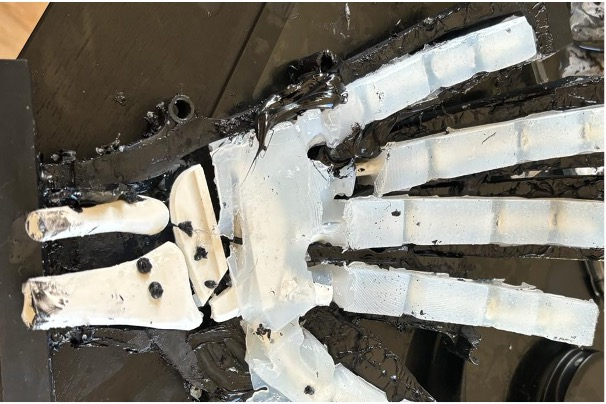
\includegraphics[width=0.8 \linewidth]{Silikonhand_Fehlversuch}}
		\caption{Silikonhand Fehlversuch}
		\label{fig:Silikonhand_Fehlversuch}			
	\end{center}
\end{figure}
\hfill \break
Jedoch gab es einen Notlösungsversuch um das vorhandene Material zu retten, dafür wurden die Finger abgeschnitten bis zu dem Punkt, an dem der Guss nicht gelungen ist, daraufhin vermessen und ein Modell wurde modelliert. Dieses ersetzt die Handfläche 
aus Silikon mit einer 3D Gedruckten und auf diese können die bestehenden Silikonfinger auf eine Einkerbung für diese gesteckt werden. In der Abbildung ist der Unterschied, zwischen Silikon und Kunststoff anhand der Farben zu sehen, dunkelgrau steht 
für das 3D-Gedruckte Modell und die beige Farbe für das Silikon. Zusehen sind auch fünf Kanäle, durch diese soll die Angelschnur gehen und an den Fingern ziehen. \\
\\
\begin{figure}[H]
	\begin{center}
		\scalebox{1.2}
		{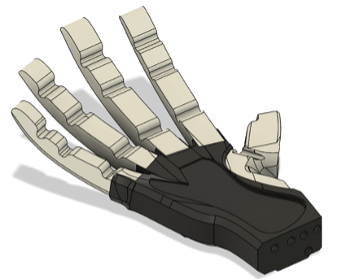
\includegraphics[width=0.8 \linewidth]{Silikonhand_Fehlversuch2}}
		\caption{Silikonhand Fehlversuch 2}
		\label{fig:Silikonhand_Fehlversuch2}			
	\end{center}
\end{figure}
\begin{figure}[H]
	\begin{center}
		\scalebox{1.2}
		{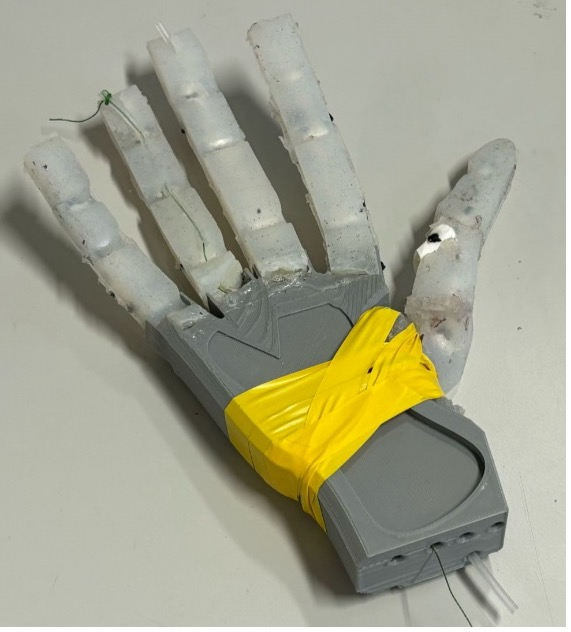
\includegraphics[width=0.8 \linewidth]{Silikonhand_Fehlversuch3}}
		\caption{Silikonhand Fehlversuch 3}
		\label{fig:Silikonhand_Fehlversuch3}			
	\end{center}
\end{figure}
\hfill \break
In der Praxis hat sich dann herausgestellt, dass die Finger sehr weich sind und daher ihr eigenes Gewicht kaum halten können. Der hat Faltmechanismus funktioniert, jedoch nicht ausreichend und in auch nicht in gewünschtem Maße. Lösen könnte man die 
Instabilität der einzelnen Fingern mit härterem Silikon. Grundsätzlich wurde moderat hartes Silikongewählt mit dem Härtefaktor 25A, das doppelte somit 50A oder mehr wären notwendig um die Finger stabil zu halten. \\
\\
Die Problematik mit dem Guss, dass das Modell sich nicht in einem gießen lässt und die Erkenntnis beim Notmodell, dass die Finger nicht stabil bleiben, hat gezeigt dass dieses Konzept für unser Projekt nicht tauglich ist. Aufgrund dieser 
Ergebnisse wird das Konzept vorerst verworfen, dennoch soll Silikon weiterhin ein Bestandteil der zukünftigen Modelle bleiben besonders aufgrund des Griffs, der damit gesichert werden kann. \\
\\

\subsubsection{Vierte Hand (Hybrid-Konzept)}
\paragraph{Erfahrung und Konzepterläuterung}
\hfill \break
\hfill \break
Aus den Versuchen der letzten Kapitel konnte einiges an Erfahrung gesammelt werden. Nun ist klar worauf bei dem Modell einer Hand geachtet werden muss. \\
Wie in Kapitel \autoref{chap:Erste Testhand} hat sich gezeigt, dass die einzelnen Fingerglieder sich kontinuierlich um die anderen Falten müssen. Auch hat sich im Kapitel „zweite Testhand“ gezeigt, wie wichtig es ist für ein Modell zu sorgen, dass einer hohen 
Last standhält und nicht brüchig ist. In den letzten Versuchen hat sich gezeigt, dass die Zugschnur an sämtlichen Stellen auf Reibung trifft. \\
\\
Entdeckt wurde eine erweiterte Version der Hand aus \autoref{chap:Zweite Testhand} von Gael Levin. Diese hat sämtliche Optimierungen, sei es die zu bemängelnde Stabilität der vorherigen Version oder auch der problematische Mechanismus der 
Zugschnüren. Im neuen Modell der "i2Hand", sind die Fingerglieder besonders an ihren Schwachstellen verstärkt worden, somit kann verhindert werden, dass die Verbindungen der einzelnen Glieder bei hoher Last oder gar der Montage brechen. Die 
Verbindungen haben vorgesehene Einkerbungen für den Kopf der Schraube oder eine Mutter, somit steht an den Seiten der Finger nichts ab. \\
Der Faltmechanismus besteht nicht mehr aus zwei Schnüre, sondern reduziert sich ausschließlich auf die Zugschnur, diese hat eine eigene Führung mit abgerundeten Kanten um die Reibung zu reduzieren. Der Rückzug wird durch eine Zugfeder verursacht, 
diese erstreckt sich durch den gesamten Finger und ist am Anfang und seinem Ende montiert. \\
\\
Doch nicht alles war ideal an dem Modell der neuen Hand, den der Motorblock wurde nicht optimiert und nutzt weiterhin den Mechanismus, in dem sich die Zugschnur um einen Aufsatz auf dem Motor wickelt. Daher muss eigens ein neuer Mechanismus 
entworfen werden in diesem soll die Drehbewegung des Servomotors in eine lineare Zugbewegung übersetzt werden. \\
\\

\paragraph{Erster Entwurf}
\hfill \break
\hfill \break
\begin{figure}[H]
	\begin{center}
		\scalebox{1.2}
		{\includegraphics[width=0.8 \linewidth]{Motorblock_v2}}
		\caption{Motorblock v2}
		\label{fig:Motorblock_v2}			
	\end{center}
\end{figure}
\begin{figure}[H]
	\begin{center}
		\scalebox{1.2}
		{\includegraphics[width=0.8 \linewidth]{Motorblock_v2_Mechanismus}}
		\caption{Motorblock v2 Mechanismus}
		\label{fig:Motorblock_v2}			
	\end{center}
\end{figure}
\hfill \break
In der \autoref{fig:Motorblock_v2} ist ein Gerüst zu sehen, dieses in Kombination mit den fünf Motoren, den zugehörigen Zahnstangen und Zahnrädern als Motorblock bezeichnet. Auf jeden Motor wird ein Zahnrad befestigt, dreht sich dieses Zahnrad bewegt es die 
in der Fassung platzierte Zahnstange. Der Mechanismus nennt sich "Rack and Pinion" (engl.) und wurde so dimensioniert um mit einer Drehung von 180 Grad die Zahnstange um 60mm zu bewegen. \\
\\
Nach dem Druck und einer ersten Inbetriebnahme hat sich die Funktionalität des Mechanismus erwiesen. Der Motor dreht sich und wandelt dies in eine lineare Zugbewegung um, auf der Zahnstange wird dann die Angelschnur montiert und somit kann an 
dieser kontrolliert gezogen werden. \\
\\

\paragraph{Verbesserungen – zweiter Entwurf}
\hfill \break
\hfill \break
Neben der Funktionalität hat sich gezeigt, dass das Modell in einer deutlich kleineren Form und raumeffizienter entworfen werden kann. Dafür spricht, dass sich die Zahnstange nur um 30mm Bewegen muss um den Finger ausreichend zu Falten. 
Dadurch konnte der Durchmesser des Zahnrades um ein Vielfaches verkleinert werden und dies bewirkt, dass die Halterung auch kleiner ausfällt. \\
\\
\begin{figure}[H]
	\begin{center}
		\scalebox{1.2}
		{\includegraphics[width=0.8 \linewidth]{Zahnstangenmechanismus_Unterarm}}
		\caption{Zahnstangenmechanismus Unterarm}
		\label{fig:Zahnstangenmechanismus_Unterarm}			
	\end{center}
\end{figure}
\hfill \break
In diesem Modell ist zu sehen, dass alle Servomotoren auf einer Höhe liegen. Diese werden auf einer Servohalterung (2) montiert, welche dann auf der Platte (1) montiert wird, aufgrund der Toleranzen des 3D-Drucks können die Halterungen mit 
Langlöchern adjustiert werden. Das Modell wurde mit der Rücksicht entworfen, Schrauben und Muttern im Modell zu versenken. \\
\\

\paragraph{Realisierung und Aufbau}
\hfill \break
\hfill \break

\paragraph{Versuche...}
\hfill \break
\hfill \break

\newpage
%--------------------------------------------------------------------------
%--------------------------------------------------------------------------
\section{Hardware Realisierung}

\subsection{Eingabesubsystem}

\subsubsection{Grundlegende Voraussetzungen \textcolor{red}{Laci}}
Die Hardware des Eingabesubsystems muss einige Kriterien erfüllen, um schlussendlich voll funktionfähig in das Gesamtsystem eingebaut 
werden zu können. Zunächst ist die Größe der Schaltung, als mit der wichtigste Punkt zu nennen. Da es bei diesem Projekt nicht nur
um die Funktionalität, sondern auch um ein ergonomisches Benutzererlebnis geht, sollte die entgültige Platine auf dem Handschuhrücken
nicht größer als 4cm x 4cm sein. Beim Design der Elektronik muss durch die Größenrestriktion natürlich darauf geachtet, dass durch
diese keine Einbußen in Bezug auf die korrekte und sichere Funktion des Projektteils entstehen. Übermäßige Wärmeentwicklung ist 
ebenfalls zu vermeiden, da diese auf lange Zeit unangenehm für den Endnutzer ist. Die Versorgung der Schaltung
sollte möglichst über einen kleinen und portablen Akku geschehen, um dem Benutzer das bestmögliche Erlebnis zu bereiten. Dieses Feature ist
allerdings optional und ist daher nicht garantiert zur Verwendung bereit. Über einen USB Anschluss soll der Mirkokontroller programmierbar sein und die Schaltung
auch für Test -und Wartungszwecke versorgt werden können. Das Maximalgewicht darf 500g nicht übersteigen. \\

\subsubsection{Überlegungen, Simulationen und Berechnungen \textcolor{red}{Laci}}
\label{chap:Überlegungen, Simulationen und Berechnungen}
\paragraph{Bewegungserfassung der Fingerbeugung}
\hfill \break
\hfill \break
Die Bewegungen des Benutzers müssen gemessen werden können. Das bedeutet, dass eine Form von Messschaltung notwendig ist um die  
Beugung der Finger interpretieren zu können. Dies könnte man durch das Messen des Beugungswinkels realisieren. Allerdings hat 
jeder Finger drei Gelenke, wodurch man diese auch bei der Roboterhand individuell steuern müsste. Die zweite Möglichkeit wäre, 
durch eine visuelle Aufnahme die Bewegung des Handschuhs und dadurch des Benutzers aufzuzeichnen. Da dies allerdings nur in dafür vorgesehenen, 
mit Kameras ausgestatteten, Räumen funktionieren würde, ist dies für uns auch keine sinnvolle Möglichkeit. Schließlich haben 
wir uns für die Erfassung der Fingerbewegungen mittels Flexsensoren entschieden. Diese ändern den Widerstand je nach der 
aktuell vorherrschenden Beugung. Bei dieser Art der Bewegungserfassung muss man nicht jedes Fingergelenk einzeln steuern und 
braucht auch keine externen Kameras. Somit ist bei dieser Methode der Datenerfassung ein sehr flexibler Verwendungsbereich 
des Handschuhs gewährleistet. Um die Änderungen der Widerstandsstreifen messen und verarbeiten zu können ist nun eine Schaltung 
notwendig. Diese muss Wertdifferenzen erkennen und in ein geeignetes Format zur Weiterverarbeitung mit einem Mikrokontroller
umwandeln können. \\
\\
\paragraph{Auslesen der Sensoren}
\label{par:Auslesen der Sensoren}
\hfill \break
\hfill \break
Das Auslesen der Flexsensoren kann durch einen einfachen Spannungsteiler erfolgen. Dabei ist die Genauigkeit
allerdings nicht optimal und ist daher nicht für unsere Anwendung geeignet. Als Lösung für dieses Problem haben wir an eine 
OPV-Messschaltung gedacht. Diese soll mit einem Shuntwiderstand die Spannungsdifferenz messen, die sich bei einer Veränderung 
des flexiblen Widerstands ergibt. Durch eine geeignete Verstärkung des OPVs kann diese mit einer Referenzspannung verglichen 
werden. \\
\begin{figure}[H]
	\begin{center}
		\scalebox{1.25}
		{\includegraphics[width=0.8 \linewidth]{Simulation_Spannungsmessung_Flexsensoren}}
		\caption{LTspice Simulation der Flexesnor - Messschaltung}
		\label{fig:Simulation_Spannungsmessung_Flexsensoren}		
	\end{center}
\end{figure}
\hfill \break
Die Flexsensoren (Rflex) beziehen ihre Versorgung über einen Shunt-Widerstand (Rs). Je nach Belastung, ändert sich der 
Spannungsabfall an diesem (Je größer die Beugung des Sensors, desto kleiner ist der Spannungsabfall). Die Spannungsdifferenz 
am Shunt-Widerstand wird von einem Operationsverstärker verstärkt. Bei der Auswahl des OPVs sind einige Punkte zu beachten, um 
eine korrerkte und genaue Erfassung der Fingerbeugung zu gewährleisten. \\
\\
Folgende Kriterien müssen folglich bei der Wahl des Operationsverstärkers beachtet werden:
\begin{itemize}
	\item Ausgangspegel bei gewählter Versorgungsspannung: \\
		  \\
		  Zunächst wurde das Kriterium der Versorgungsspannung betrachtet. Da wir maximal 5V Gleichspannung in der gesamten 
		  Schaltung verwenden wollen, muss der OPV mit dieser geringen Spannung immer noch verstärken. Da am positiven 
		  Verstärkereingang eine maximale Spannung von 3.3V anliegt, muss dies bei Verstärkern mit einer geeigneten Supply Range 
		  auch mit nur 5V Versorgungsspannung gewährleistet sein.
	\item Referenzspannung: \\
		  \\
		  Ein weiteres Kriterium ist das vorhanden sein eines Referenzspannungsanschlusses. Da der OPV keine Rail-to-Rail 
		  Technologie besitzt, muss der Ausgangsspannungspegel auf ein gewisses minimum angehoben werden. In unserem ist dies 
		  +1V. Würde diese Refernzspannung nicht vorhanden sein, so würde der OPV falsche Werte erzeugen, da dieser erst ab einer
		  verstärkten Spannung am Ausgang von ca. 750mV korrekt funktioniert.

\end{itemize}
Aufgrund dieser Kriterien und der Notwendigkeit von Genauigkeit und geringer Störungseigenschaften, viel die Wahl des 
Operationsverstärkers auf den INA129 instrumentation amplifier. \\
\\
Der Shunt-Widerstand wurde nicht berechnet. Dieser wurde einfach durch probieren inder Simulation bestimmt. \\
\\
Ein Tiefpassfilter (Rf und Cf) ist hinter den Ausgang des OPVs geschaltet, um mögliche Spannungsstörungen (Ripple), zusätzlich
zu dem ohnehin schon sehr störungsarmen Ausgangssignal des INA129, herauszufiltern. Der zu GND geschaltete Widerstand (R1), 
entlastet den Eingang des folgenden ADCs. Der Tiefpassfilter wurde folgendermaßen dimensioniert. \\
\\
\paragraph{Berechnung des Tiefpassfilters}
\hfill \break
\hfill \break
\hspace*{1cm} $f_{g} = 20 kHz $ \hspace*{1cm} $\tau = \frac{1}{\omega_{g}} = \frac{1}{2\pi * 20 kHz} $ \\
\\
\hspace*{1cm} $f_{g} = \frac{\omega_{g}}{2\pi} $ \hspace*{1.7cm} $\tau = R * C $ \\
\\
\hspace*{4.25cm} $ C = 68 nF $ \hspace*{1cm} $ R = \frac{\tau}{68nF} = 117 \Omega $ \\
\\
\paragraph{Berechnung der OPV Verstärkung und Dimensionierung des Shuntwiderstands}
\hfill \break
\hfill \break
\hspace*{1cm} Verstärkungsgleichung laut Datenblatt: $ G = 1+\frac{49.4k\Omega}{R_{g}} $ \\
\\
\hspace*{1cm} Gain gewählt mit 46. \hspace*{1cm} $ R_{g} = 1.1k\Omega $ \\
\\
Die Verstärkung wurde so gewählt, dass diese mit dem Shunt-Widerstand für den ADC optimal geeignet ist.
Der Shunt-Widerstand wurde mithilfe der Simulation in \autoref{fig:Simulation_Spannungsmessung_Flexsensoren}
gewählt. \\
\\
Der Shuntwiderstand wurde nicht wirklich berechnet. Dieser wurde durch probieren in der Simulation ermittelt. Eine Berechnung
des Shunts wäre nicht wirklich Zielführend gewesen, da diese normalerweise bei Schaltungen mit hohen Strömen verwendet werden. 
Da sich die Flexsensoren allerdings in einem Widerstandsbereich von $25k\Omega$ - $125k\Omega$ befinden, benötigen diese nicht
viel Strom, wodurch schon zu erwarten war, dass ein relativ hoher Wert benötigt wird. Schlussendlich wurden $240\Omega$ gewählt,
da dieser Widerstand bei sowohl voller, als auch geringer Biegung der Flexsensoren, eine gute Spannungsdifferenz für die 
Verstärkung mit dem OPV liefert. \\
\\
\paragraph{Umwandlung der Differenzwerte in ein geeignetes Format}
\label{par:Umwandlung der Differenzwerte in ein geeignetes Format}
\hfill \break
\hfill \break
Um nun die analogen Ausgangswerte des Operationsverstärkers nach der Verstärkung der Spannungsdifferenzen am Flexsensor für
den Mikrokontroller möglichst effizient und brauchbar zu machen, ist eine Umwandlung in ein digitales Signal notwendig.
Dies Funktion wird mit mit einem ADC umgesetzt. Bei der Wahl dieses Logikbauteils, sind, wie beim OPV, einige Kriterien zu 
beachten um die korrekte Funktion der Schaltung weiterhin zu gewährleisten. \\
\\
Folgende drei Kriterien sind maßgeblich bei der Wahl der Analog-Digital-Wandlers zu beachten:
\begin{itemize}
	\item Genauigkeit, Auflösungund Aussteuerbereich: \\
		  \\
		  \hspace*{1cm} $ Aussteuerbereich = 0 - 3.3V $ \\
		  \\
		  \hspace*{1cm} bei 10Bit ADC: $ LSB = 3.22mV $ \\
		  \\
		  \hspace*{1cm} Wegen der 1V Referenzspannung des OPVs ist der Ausgangspegel 1V - 3.3V \\
		  \\
		  \hspace*{1cm} $ ADC Ausgangsstufen = \frac{2.3V}{3.22mV} = 713 $ \\
\end{itemize}
Der reale Ausgangspegel des OPVs liegt, wie bei der Simulation in \autoref{par:Auslesen der Sensoren} ermittelt, zwischen 1.277V bis 2.416V.
Das beudeutet, dass eine Auflösung von 10Bit und ein Austeuerbereich von 0V - 3.3V ausreichend ist, um den kompletten Wertebereich
sehr genau abzudecken. Zusätzlich haben wir uns noch dazu entschieden alle Logikbauteile die eine Kommunikation mit dem Mikrokontroller
erfordern mit dem I2C Bussystem anzuschließen. Daher muss der Analog-Digital-Wandler diese Art der Kommunikation ebenfalls unterstützen.
Aufgrund dieser Auswahlkriterien ist die Wahl des Bauteils auf den MAX11611 gefallen.\\
\\
\paragraph{Vervielfachung der Schaltung für alle Flexsensoren}
\hfill \break
\hfill \break
Um die zuvor beschriebene Schaltung nun nicht für jeden Flexsensor einzeln bauen zu müssen, wäre eine Art Schalter vorteilhaft.
Dieser soll in Sekundenbruchteilen zwischen allen Sensoren durchschalten. Das bedeutet also, dass zwischen dem Shunt-Widerstand
und $R_{flex}$ in der Simulation dieses Bauteil platziert werden muss. \\
\\
Für diesen Zweck ist ein Multiplexer bestens geeignet. Folgende Kriterien muss dieser erfüllen.
\begin{itemize}
	\item Versorgung und Kanäle: \\
		  \\ 
		  Die Versorgung muss an den Rest der Schaltung angepasst sein, das bedeutet, dass entweder 3.3V oder 5V in Frage kommen.
		  Bei einer Anzahl von einem Flexsensor pro Finger, also fünf, muss der Multiplexer mindestens 5 Kanäle aufweisen, wobei 
		  mehr Kanäle für mögliche zukünftige Erweiterungen kein Problem sind. All diese Eingänge müssen auf einen Ausgang geschalten
		  werden.
	\item Ansteuerung: \\
		  \\ 
		  Die Ansteuerung muss mit einem Mikrokontroller möglich sein. Hier bleibt also die Wahl zwischen analogen und digitalen 
		  Anschlüssen, oder ein I2C Anschluss um mit dem Rest der Schaltung kompatibel zu bleiben.
\end{itemize}
Folglich viel die Wahl auf den MUX508IDR. Dieser ist ein 8:1 Channel Multiplexer, der über 5V versorgt werden kann und über drei 
Analoganschlüsse für die Auswahl des Kanals verfügt. \\
\\
\paragraph{Bewegungserfassung der Handgelenksdrehung}
\hfill \break
\hfill \break
Um die Drehung des Handgelenks zu erfassen ist ein anderer Sensor als ein Flexsensor notwendig. Dieser neue Sensor muss die 
Funktion eines Gyroskops haben und folglich die Positionen von X, Y -und Z-Achse übermitteln. Dieser Übermittlung muss per
I2C-Bus erfolgen, um die Kompatiblität mit der restlichen Schaltung zu ermöglichen. \\
\\
Ausgewählt wurder der Sensor MPU-6000, da dieser schon eingebaute ADCs hat, um die Achswerte vor der Übertragung zu digitalisieren. \\
\\
\paragraph{Mikrokontroller}
\label{par:Mikrokontroller}
\hfill \break
\hfill \break
Bei der Auswahl des Mikrokontrollers wurden sehr viele Aspekte beachtet. Dieser ist das Herzstück der Schaltung und ermöglicht
allen Komponenten zusammen zu funktionieren und diese auch zu steuern. \\
\\
Folgende Kriterien müssen vonn dem verwendeten Mikrokontroller folglich erfüllt werden:
\begin{itemize}
	\item Performancerelevante Ressourcen: \\
		  \\
		  Zu beachten ist hierbei vor allem der vorhandene Flash-Speicher, die CPU und der On-Chip Memory. Hierbei gilt grundsätzlich 
		  natürlich je mehr, desto besser. Das gleiche gilt ebenfalls für den Flash-Speicher.
	\item Versorgung und Anschlüsse: \\
		  \\
		  Um mit der Schaltung kompatibel zu sein, muss der Mikrokontroller mit 3.3V oder 5V versorgt werden können. Zusätzlich
		  sollte der Chip möglichst wenig Leistung brauchen. Es sollten mindestens zehn I/O-Anschlüsse vorhanden sein.
	\item Unterstützte Bussysteme: \\
		  \\
		  Da die wir bei der Schaltung eunheitlich auf das I2C Bussystem setzen, muss zumindest dieses von dem gewählten Mikrokontroller
		  unterstützzt werden. Als zweite Pflichtunterstützung gilt die UART-Kommunikation. Die Funktion und Notwendigkeit dieser,
		  wird in \autoref{par:Externe Anschlüsse} erläutert.
	\item Möglichkeiten der drahtlosen Übertragung: \\
		  \\
		  Da die Flexsensorwerte drahtlos Übertragen werden müssen, muss der Mikrokontroller eine Form dieser Übertragung unterstützen.
		  Vorzüglicherweise ist die Antenne für die Übertragung schon vorhanden, damit weitere Schaltungsteile nicht notwendig sind.
		  Hier kämen zum Beispiel Bluetooth oder Wifi in Frage.
	\item Programmierbarkeit: \\
		  \\
		  Der Chip muss mit einer schon verfügbaren Entwicklungsumgebung programmierbar sein. Wichtig ist in diesem Bezug vor allem
		  die Debugmöglichkeit, da bei einigen Mikrokontrollern ein extra Debugtool um viel Geld erworben werden muss. Eine Programmierung
		  im Terminal kommt ebenfalls nicht in Frage.
	\item Größe und Formfaktor: \\
		  \\
		  Schlussendlich dürfen sich alle Kriterien jedoch nicht zu sehr auf die Größe des Mikrokontrollers auswirken. Diese sollte
		  natürlich so klein wie möglich sein und trotzdem Bauteile wie eine Antenne aufweisen.
\end{itemize}
Nach beachtung aller Kriterien haben wir uns für einen ESP32 Mikrokontroller entschieden. Hierbei blieb allerdings die Wahl zwischen
dem reinen Chip und dem Modul, bei dem die Antenne und andere Funktionalitäten, die andernfalls selbst gebaut werden müssten,
schon integriert sind. Nach Abwägungen von Größe und Performance, haben wir uns für das ESP32-WROOM-32E-N16 Modul entschieden.
Dieses hat eine integrierte Antenne, reichlich Performance und viel Flash-Speicher. Der Formfaktor ist bei allen diesen 
Funktionalitäten immer noch im Rahmen. \\
\\
\paragraph{\textcolor{red}{Akkuversorgung}}
\hfill \break
\hfill \break
Da es nicht praktikabel ist die Schaltung des Handschuhs dauerhaft mit einem Kabel zu versorgen, soll dies schlussendlich durch
einen Akku oder eine Batterie erfolgen. Entschieden haben wir uns für eine Lithium-Polymer-Akku (LiPo), da diese trotz geringer 
größe verglichen mit anderen Akkuarten eine hohe Kapazität besitzen. \\
\\
Die notwendige Kapazität für eine bestimmte Betriebsdauer wurde folgendermaßen berechnet:
\textcolor{red}{Berechnung Akkukapazität hier einfügen}
\\
Um den LiPo-Akku nicht jedes mal extern aufladen zu müssen, haben wir uns eine Schaltung überlegt, die dies auch mithilfe des
schon vorhandenen USB-C Anschlusses für das Programmieren des Mikrokontrollers verwendet wird. Dazu ist allerdings eine relativ 
komplitzierte Schaltung notwendig, weswegen bei vielen Produkten, die LiPo-Akkus verwenden, extra Ladegeräte gekauft werden müssen.
Dies wollten wir vermeiden und haben dementsprechend viel Zeit in die Reserche für eine funktionierende LiPo-Kontroller-Schaltung
investiert. \\
\\
Zunächst ist jedoch wichtig zu wissen, welchen Akku wir überhaupt erwenden. Entschieden haben wir uns für den \textcolor{red}{LiPo-Akku}.
\\

\subsubsection{Versuchsaufbauten und Messungen \textcolor{red}{Laci}}
In den folgenden Punkten, werden die praktischen Tests der, in \autoref{chap:Überlegungen, Simulationen und Berechnungen} beschriebenen Konzepte und Überlegungen, erläutert.\\
\paragraph{Messchaltung der Flexsensoren}
\hfill \break
\hfill \break
Zunächst wurde die Schaltung aus \autoref{par:Auslesen der Sensoren} auf einem Steckbrett aufgebaut. Das Ziel der Messung ist es, den Widerstand 
bei jeder Stellung eines Flexsensoren zu wissen. Dies ist wichtig, um die Daten der Sensoren korrekt auszulesen und an die 
Roboterhand zu senden. Werden die Widerstandswerte nicht korrekt gemessen, so bewegt sich die Roboterhand nicht entsprechend 
nach den Bewegungen des Benutzers. \\
\\
Die zu messende Größe ist die Ausgangsspannung des OPVs, die sich je nach Widerstand der Last verändert. Die Last wird in 
unserem Versuchsaufbau von drei Widerständen simuliert, da wir die Flexsensoren zu dem Zeitpunkt der Messung noch nicht zu 
Verfügung hatten. Wir haben die Lastwiderstände mit 27k, 68k und 118k gewählt, da der Widerstandsbereich der Sensoren bei 
25k – 125k liegt. In \autoref{par:Messergebnisse} werden die Messergebnisse dargestellt. \\
\\
\begin{figure}[H]
	\begin{center}
		\scalebox{1.0}
		{\includegraphics[width=0.8 \linewidth]{Steckbrettaufbau_Spannungsmessung_INA129}}
		\caption{Steckbrettaufbau der Flexesnor - Messschaltung}
		\label{fig:Steckbrettaufbau_Spannungsmessung_INA129}	
	\end{center}
\end{figure}
\hfill \break
\hfill \break
\begin{figure}[H]
	\begin{center}
		\scalebox{1.0}
		{\includegraphics[width=0.8 \linewidth]{Bild_Einstellungen_Netzteil}}
		\caption{Netzteileinstellungen}
		\label{fig:Bild_Einstellungen_Netzteil}	
	\end{center}
\end{figure}
\hfill \break
+3.3V für die Versorgung des Flexsensors (Last), simuliert mit drei normalen Widerständen.\\
+1V als Referenzspannung für den INA-129.\\
+5V zur Versorgung des INA129.\\
\\

\paragraph{Messergebnisse}
\label{par:Messergebnisse}
\hfill \break
\hfill \break
\begin{figure}[H]
	\begin{center}
		\scalebox{1.2}
		{\includegraphics[width=0.8 \linewidth]{Oszibild_RL_27k}}
		\caption{Oszilloskopbild mit $R_{L} = 27k\Omega$}
		\label{fig:Oszibild_RL_27k}		
	\end{center}
\end{figure}
Das obige Oszilloskopbild zeigt die, mit einem Tastkopf, gemessene Ausgangsspannung des Operationsverstärkers, bei einem Flexsensorwiderstand
von 27k$\Omega$. Die gemessene Spannung ist rot eingekreist und beträgt 2.28V. Da bei der Simulation in LTspice mit einem Widerstand 
von 25k$\Omega$ eine Ausgangsspannung von 2.416V resultierte, ist anzunehmen, dass 2.28V 
für den gewählten Widerstand angemessen sind. Daraus kann man schließen, dass die Schaltung
für diesen Widerstandswert des Flexsensors korrekt funktioniert.
\\
\begin{figure}[H]
	\begin{center}
		\scalebox{1.0}
		{\includegraphics[width=0.8 \linewidth]{Oszibild_RL_67k}}
		\caption{Oszilloskopbild mit $R_{L} = 67k\Omega$}
		\label{fig:Oszibild_RL_67k}		
	\end{center}
\end{figure}
\hfill \break
Nun wurde die gleiche Messung erneut durchgeführt, allerdings mit einem Flexsensorwiderstand
von 67k$\Omega$. Wir zu erwarten, ist die Ausgangsspannung des OPVs gesunken, da der 
Spannungsabfall am Shuntwiderstand nun geringer ausfällt. Zu erwarten war ein Spannungswert
von rund 1.5V. Dieser Pegel wurde mit 1.52V fast genau getroffen, wodurch die funktionsfähigkeit
der Schaltung weiter sichergestellt wurde.
\begin{figure}[H]
	\begin{center}
		\scalebox{1.0}
		{\includegraphics[width=0.8 \linewidth]{Oszibild_RL_118k}}
		\caption{Oszilloskopbild mit $R_{L} = 118k\Omega$}
		\label{fig:Oszibild_RL_118k}		
	\end{center}
\end{figure}
\hfill \break
Schlussendlich wurde noch ein Flexsensorwiderstand von 118k$\Omega$ simuliert, um den
nahezu Maximalwert des Sensors zu simulieren. Zu erwarten waren rund 1.3V. Die Messung
bestätigt die Überlegungen, wodurch die Funktionalität dieser Schaltungskomponente bewiesen
wurde. \\
\\
Zusätzlich ist nun die Notwendigkeit einer Referenzspannung von +1V bewiesen worden, da
ohne dieser ein theoretischer Spannungspegel von nur 500mV am Ausgang des INA-129 aufgetreten
wäre.  Dies ist praktisch allerdings nicht möglich, da der OPV über keine Rail-to-Rail
Technologie verfügt, wodurch er nur eine minimale Ausgangsspannung von rund 800mV ausgeben 
kann.
\\

\newpage
\subsubsection{Schaltungsdesign \textcolor{red}{Laci}}
Nach den generellen Überlegungen und Versuchsaufbauten, die zu der Entwicklung der Schaltung des Eingabesubsystems beigetragen haben, wird in diesem Punkt 
das genaue Schaltungsdesign erläutert. \\
\\
\paragraph{Externe Anschlüsse}
\label{par:Externe Anschlüsse}
\hfill \break
\hfill \break
\begin{itemize}
	\item Anschluss zur Programmierung des Mikrokontrollers: \\
		  \\
		  Für die Programmierung des Mikrokontrollers wird ein USB Anschluss benötigt. Dieser sollte möglichst kompatibel mit
		  den neuesten Computern sein, weswegen wir uns für USB-C-Typ2.0 entschieden haben. Um das Serial Signal der USB Schnittstelle
		  für den Mikrokontroller lesbar zu machen, muss dieses für die UART-Kommunikation umgewandelt werden. Hierzu muss der Mikrokontroller
		  diese auch unterstützen. Mit einer Serial-UART-Bridge, wird das Signal umgewandelt. Der Chip wird von +3.3V versorgt.
		  Von der USB-Buchse werden die beiden Datenleitungen D+ und D- mit verbunden. Anschließend wird das umgewandelte Signal 
		  über die UART-Leitungen an den ESP32 Mikrokontroller übertragen. Wichtig zu beachten ist hierbei, dass die UART-Leitungen
		  ausgekreuzt sein müssen. Die Funktion der Anschlüsse RTS und DTR wird in \autoref{par:Mikrokontroller} erläutert. \\
		  \begin{figure}[H]
			\begin{center}
				\scalebox{0.5}
				{\includegraphics[width=0.8 \linewidth]{USB_C_Schaltplan_Handschuh}}
				\caption{USB-C-Buchse}
				\label{fig:USB_C_Schaltplan_Handschuh}				
			\end{center}
		\end{figure}
	\item Anschluss der Flexsensoren: \\
		  \\
		  Die Flexsensoren könnten natürlich einfach angelötet werden, jedoch ist die einfache Wartung bei einem fehlerhaften
		  Sensor ebenfalls zu berücksichtigen. Aufgrund dessen wird eine 6-Pin-JST-Buchse als Anschluss verwendet. Alle GND-Pins
		  werden auf einen zusammengefasst, um möglichst viel Platz zu Sparen. \\
		  \begin{figure}[H]
			\begin{center}
				\scalebox{0.5}
				{\includegraphics[width=0.8 \linewidth]{JST_Flexsensoren_Schaltplan_Handschuh}}
				\caption{Flexsensor Connector}
				\label{fig:JST_Flexsensoren_Schaltplan_Handschuh}				
			\end{center}
		\end{figure}
	\item \textcolor{red}{Anschluss des Akkus:} \\
		  \\
		  Der Akku wird ebenfalls mit einer JST-Buchse mit der Schaltung verbunden anstatt diesen anzulöten. Da der Akku einen
		  Versorgungs -und GND-Anschluss hat, wird eine 2-Pin-JST-Buchse verwendet. \\
		  \begin{figure}[H]
			\begin{center}
				\scalebox{0.5}
				{\includegraphics[width=0.8 \linewidth]{JST_Akku_Schaltplan_Handschuh}}
				\caption{Akku Connector}
				\label{fig:JST_Akku_Schaltplan_Handschuh}				
			\end{center}
		\end{figure}\end{itemize}

\paragraph{Mikrokontroller} 
\hfill \break
\hfill \break
Der ESP32-Chip wird mit +3.3V versorgt. Wichtig zu beachten ist dadurch, das ein Logic-HIGH somit auch 3.3V und nicht 5V ist!
Die Versorgung wird mit einem Kondensator stabilisiert. Für alle Busleitungen, also I2C und UART, wurden Widerstände in Serie
hinzugefügt, um die Kommunikationsleitungen vor Spannungsspitzen oder Überspannung zu schützen. Die Funktion wäre auch ohne diese
gegeben. Für die Datenleitungen SDA und SCL des I2c Busses sind zwei $10k\Omega$ PullUp-Widerstände vorgesehen. Zusätzlich 
wird ebenfalls der Anschluss IO16 mit einem PullUp-Widerstand auf 3.3V gezogen, da dies so vom Datenblatt vorgegeben wird. 
Die Funktionen der einzelnen Anschlüsse werden in den folgenden Punkten gemeinsam mit den damit verbundenen Bauteilen näher erläutert. \\
\begin{figure}[H]
	\begin{center}
		\scalebox{0.5}
		{\includegraphics[width=0.8 \linewidth]{ESP32_Schaltplan_Handschuh}}
		\caption{ESP32 Mikrokontroller}
		\label{fig:ESP32_Schaltplan_Handschuh}	
	\end{center}
\end{figure}

\paragraph{Mikrokontroller Buttons}
\label{par:Mikrokontroller Buttons}
\hfill \break
\hfill \break
In der Schaltung sind drei Taster verbaut. Diese sind alle mit dem Mikrokontroller verbunden und erfüllen verschiedene Funktionen.
\begin{itemize}
	\item Upload Button: \\
		  \\ 
		  Dieser Button ist mit dem IO0 Anschluss des ESP32 verbunden und muss bei dem Hochladen von Code kurzzeitig gedrückt 
		  werden, um den Mikrokontroller in den Upload-Modus zu versetzen. Der Pin IO0 ist standardmäßig für diese Funktion vorgesehen
		  und sollte für nichts anderes verwendet werden. 
	\item Reset Button: \\
		  \\
		  Dieser Button ist mit dem EN (Enable) Anschluss des ESP32 verbunden. Die Funktion dieses Tasters ist es, den ESP32 jederzeit 
		  zurücksetzen zu können falls dieser abstürtzt oder ein anderweitiges Problem auftritt, durch das dieser nicht mehr korrekt
		  funktioniert.
	\item Progrmmable Button: \\
		  \\
		  Die Funktion dieses Buttons kann frei durch den programmierten Code gewählt werden. 
\end{itemize}

\paragraph{Status LEDs}
\hfill \break
\hfill \break
Die beiden Leuchtdioden sind als Statusanzeige gedacht. Eine POWER LED, die immer leuchtet wenn die Schaltung mit +5V
versorgt wird. Die Funktion der anderen LED ist, sowie bei einem Button, frei wählbar und ist deswegen mit Pin IO13 des ESP32
verbunden. \\
\begin{figure}[H]
	\begin{center}
		\scalebox{0.5}
		{\includegraphics[width=0.8 \linewidth]{LEDs_Schaltplan_Handschuh}}
		\caption{Status LEDs}
		\label{fig:LEDs_Schaltplan_Handschuh}		
	\end{center}
\end{figure}

\paragraph{Multiplexer}
\hfill \break
\hfill \break
Der Multiplexer schaltet zwischen allen Flexsensoren durch und vermeidet somit die Messschaltung fünf mal bauen zu müssen. 
Die Verbindung zum ESP32 erfolgt über drei digitale Addresspins und einen Enable Pin. Je nachdem welche Bitkombination übermittelt
wird, ändert sich die interne Schalterposition und somit der gerade aktive Kanal zur Messung eines Flexsensors. \\
\\
\begin{figure}[H]
	\begin{center}
		\scalebox{0.5}
		{\includegraphics[width=0.8 \linewidth]{Multiplexer_Schaltplan_Handschuh}}
		\caption{Multiplexer}
		\label{fig:Multiplexer_Schaltplan_Handschuh}		
	\end{center}
\end{figure}

\paragraph{Operationsverstärker}
\hfill \break
\hfill \break
Für das Auslesen der Flexsensoren, wird eine Schaltung, wie in \autoref{par:Auslesen der Sensoren} beschrieben, benötigt. Da am
Shuntwiderstand nur sehr wenig Spannungsabfall auftritt und daher die Spannungsdifferenz zwischen positivem und negativem 
Verstärkereingang sehr klein ist, muss das Signal verstärkt werden. Hierfür wird der INA129 Instrumentenverstärker verwendet.
Dieser wird mit 5V versorgt, was für einen OPV eine relativ geringe Versorgungsspannung ist. Da die maximale Eingangsspannung
der Verstärkereingänge allerdings nie mehr als 3.3V beträgt, ist dies kein Problem. \\
\\
Die +1V Spannungsreferenz ist notwendig, da der ausgewählte Operationsverstärker nicht über Rail-to-Rail Technologie besitzt. 
Die kleinstmögliche Spannungsdifferenz am Eingang des OPV, wenn der Flexsensor seinen maximalen Widerstand von
$125k\Omega$ erreicht, beträgt nur 6.3mV. Aufgrund der fehlenden Rail-to-Rail Fähigkeit, muss die Ausgangsspannung des OPV deshalb
auf mindestens 800mV angehoben werden, um eine korrekte Funktion des OPVs zu gewährleisten. Deshalb wird eine Referenzspannung
von 1V verwendet. \\
\begin{figure}[H]
	\begin{center}
		\scalebox{0.5}
		{\includegraphics[width=0.8 \linewidth]{Operationsverstärker_Schaltplan_Handschuh}}
		\caption{Operationsverstärker - Schaltung}
		\label{fig:Operationsverstärker_Schaltplan_Handschuh}		
	\end{center}
\end{figure}

\paragraph{Analog-Digital-Wandler}
\hfill \break
\hfill \break
Der Analog-Digital-Wandler ist dafür zuständig, die analogen Werte, vom Ausgang des Operationsverstärkers kommend, in digitale 
Signale umzuwandeln. Der OPV und der ADC sind über das Label toADC verbunden. Da der Chip über 3.3V versorgt wird, befindet
sich der mögliche Aussteuerbereich zwischen 0V und 3.3V. Wie im \autoref{par:Umwandlung der Differenzwerte in ein geeignetes Format} berechnet, 
hat der ADC in unserer Schaltung ein LSB von 3.22mV. Da wir wissen, dass die kleinste Spannungsdifferenz am Shuntwiderstand 6.3mV
ist und diese auch noch mit dem Faktor 46 verstärkt wird, kann festgestellt werden, dass der ADC mehr als genau genug für unsere
Anwendung ist. Dies ist ein Vorteil, da bei der Programmierung anschließend nicht zwischen einzelnen ADC-Stufen unterschieden werden
muss, sondern immer mehrere LSBs Unterschied auftritt. Die aktualisierten Werte, werden über die beiden I2C Leitungen an den 
Mikrokontroller übertragen. \\
\\
\begin{figure}[H]
	\begin{center}
		\scalebox{0.5}
		{\includegraphics[width=0.8 \linewidth]{ADC_Schaltplan_Handschuh}}
		\caption{ADC - Schaltung}
		\label{fig:ADC_Schaltplan_Handschuh}	
	\end{center}
\end{figure}

\paragraph{Gyroskop-Sensor}
\hfill \break
\hfill \break
Der Gyroskopsensor ist dafür zuständig die Drehung des Handschuhs in X, Y -und Z Richtung warzunehmen. Die Versorgung basiert 
auf 3.3V und die Datenübertragung erneut mittels I2C-Bussystem. Der Unterschied bei diesem Chip ist allerdings, dass mehrere ADCs
integriert sind, um die Positionsdaten der Achsen schon digitalisiert an den Mikrokontroller zu übergeben. AD0 wird dabei verwendet
um die Adresse des Mikrochips festzulegen. Diese wird später benötigt um mit dem Sensor Daten austauschen zu können.
\\
\begin{figure}[H]
	\begin{center}
		\scalebox{0.5}
		{\includegraphics[width=0.8 \linewidth]{Gyro_Schaltplan_Handschuh}}
		\caption{Gyroskopsensor - Schaltung}
		\label{fig:Gyro_Schaltplan_Handschuh}		
	\end{center}
\end{figure}
\hfill \break
Am Pin CLKIN hätte man die Möglichkeit einen externen Referenztaktgeber anzuschließen. Bei unserer Anwendung ist der integrierte 
Taktgeber allerdings völlig ausreichend, weswegen der Anschluss mit GND verbunden und damit deaktiviert wurde. Der CS Pin wird nur
für die SPI Kommunikation benötigt, weshalb dieser ebenfalls deaktiviert wurde. Das gleiche gilt für den Anschluss FSYNC. Die beiden
AUX-Anschlüsse könnte man verwenden, um mit anderen I2C fähigen Sensoren direkt zu kommunizieren. Da dies allerdings unser einziger
Sensorchip mit dieser Fähigkeit ist, bleiben die beiden Pins auch nicht verbunden. Die Kondensatoren sind vom Hersteller im Datenblatt
vorgesehen und gewährleisten einen stabilen Betrieb. \\
\\
\paragraph{\textcolor{red}{Akku Versorgung}}
\hfill \break
\hfill \break
\begin{figure}[H]
	\begin{center}
		\scalebox{0.5}
		{\includegraphics[width=0.8 \linewidth]{Akku_Controller_Schaltplan_Handschuh}}
		\caption{Akku - Controller}
		\label{fig:Akku_Controller_Schaltplan_Handschuh}	
	\end{center}
\end{figure}

\begin{figure}[H]
	\begin{center}
		\scalebox{0.5}
		{\includegraphics[width=0.8 \linewidth]{Akku_Boostconverter_Schaltplan_Handschuh}}
		\caption{Akku - Boostconverter}
		\label{fig:Akku_Boostconverter_Schaltplan_Handschuh}		
	\end{center}
\end{figure}

\begin{figure}[H]
	\begin{center}
		\scalebox{0.5}
		{\includegraphics[width=0.8 \linewidth]{Akku_Buckconverter_Schaltplan_Handschuh}}
		\caption{Akku - Buckconverter}
		\label{fig:Akku_Buckconverter_Schaltplan_Handschuh}		
	\end{center}
\end{figure}

\subsubsection{Platinendesign \textcolor{red}{Laci}}
\paragraph{Erste Testplatine}
\hfill \break
\hfill \break
Die erste Testplatine wurde in der schuleigenen Werkstatt, mithilfe einer Platinenfräse,
gefertigt. Da das Design auch zu dem frühen Zeitpunkt des Projekts schon relativ kompliziert
war, gab es bei der Fertigung einige Probleme. Aufgrund schon vorhandener Erfahrung,
wurden die Bauteile mit möglichst großem Fottprint (1206) gewählt, um ein einfaches Löten
per Hand zu ermöglichen. Da es ICs aber leider nur in einer, für das Bauteil festgelegten,
Größe zu kaufen gibt, mussten Leiterbahnen mit einer Breite von nur 0.3mm verwendet
werden. Dies führte beim Löten leider zum Ablösen dieser, weshalb einige Jumper-Kabel
notwendig waren, um die kaputten Leiterbahnen zu ersetzen. Die Installation dieser Ersatzkabel,
hat einige Zeit in Anspruch genommen, wodurch der Entwicklungsprozess der Hardware
kurzzeitig verzögert wurde. \\
\\
\begin{figure}[H]
	\begin{center}
		\scalebox{0.8}
		{\includegraphics[width=0.8 \linewidth]{Platine_Handschuh_oben_v1}}
		\caption{Platinenoberseite - erste Testplatine - Eingabesubsystem}
		\label{fig:Platine_Handschuh_oben_v1}		
	\end{center}
\end{figure}
\hfill \break
Zu sehen ist die Oberseite der ersten Testplatine des Eingabesubsystems. In der oberen linken Ecke des Bilds, sind die Anschlüsse für die 5 Flexsensoren zu sehen. Diese werden für Testzwecke mit 
Jumper-Kabeln verbunden, um ein schnelles Auswechseln der Sensoren und einsetzen von fixen Referenzwidersänden zu ermöglichen. Bei der Fertigung der Platne sind einige Leiterbahnen sehr dünn ausgefallen, 
weshalb einige Kabel zur erneuten Verbindung von Lötpads gebraucht wurden. Zu dem frühen Entwicklungszeitpunkt, wurde noch eine Micro-USB-Buchse verwendet, da diese größere Pins hat und das Löten somit erleichtert. \\
\\

\begin{figure}[H]
	\begin{center}
		\scalebox{0.8}
		{\includegraphics[width=0.8 \linewidth]{Platine_Handschuh_unten_v1}}
		\caption{Platinenunterseite - erste Testplatine - Eingabesubsystem}
		\label{fig:Platine_Handschuh_unten_v1}	
	\end{center}
\end{figure}
\hfill \break
An der Unterseite, kann der Grund für die Fehler in der Fertigung erkannt werden. Da die verwendeten ICs mit einer maximalen Leiterbahnbreite von 0.3mm verbunden werden müssen, kam es, vor allem bei der Serial-UART-Bridge in der
oberen linken Ecke des Bilds, zu Leiterbahnablösungen. Das blaue und rote Kabel stellt die Versorgung der Platine dar. 

\paragraph{Zweite Version der Platine}
\hfill \break
\hfill \break
Bei dem Design der zweiten Platinenversion, wurden schon einige Anforderungen für die Integration in das Gesamtsystem
berücksichtigt. Zu nennen sind hier beispielsweise die Abmessungen, die Konnektivität und die visuelle Darstellung 
von Parametern für den Benutzer. 

\begin{figure}[H]
	\begin{center}
		\scalebox{0.8}
		{\includegraphics[width=0.8 \linewidth]{Platinenlayout_Handschuh_oben_v2}}
		\caption{Toplayer des zweiten Platinenlayouts}
		\label{fig:Platinenlayout_Handschuh_oben_v2}		
	\end{center}
\end{figure}
\hfill \break
In \autoref{fig:Platinenlayout_Handschuh_oben_v2}, ist der Toplayer des zweiten Platinenlayouts in KiCad (siehe \autoref{chap:KiCad}) zu sehen.
Der Großteil des Platzes wird vom Mikrokontroller, dem ESP32, eingenommen. An diesen sind alle anderen Komponenten angeschlossen. Wie in 
\autoref{par:Mikrokontroller Buttons} erläutert, sind zwei Buttons zur Steuerung des ESPs vorgesehen. Mit einem $R$ ist der Reset-Button markiert
mit einem $B$ der Upload-Button. \\
\\
In der linken oberen Ecke der \autoref{fig:Platinenlayout_Handschuh_oben_v2}, sind die Anschlüsse für die Flexsensorem zu sehen. Recths daneben
ist die USB-C-Buchse platziert. Außer den genannten Bauteilen, sind nur mehr die beiden Leuchtdioden, zur Visualisierung für den Benutzer, auf dem 
Toplayer angebracht. \\
\\
\begin{figure}[H]
	\begin{center}
		\scalebox{0.8}
		{\includegraphics[width=0.8 \linewidth]{Platinenlayout_Handschuh_unten_v2}}
		\caption{Bottomlayer des zweiten Platinenlayouts}
		\label{fig:Platinenlayout_Handschuh_unten_v2}		
	\end{center}
\end{figure}
\hfill \break
In \autoref{fig:Platinenlayout_Handschuh_unten_v2}, ist der Bottomlayer der zweiten Platinenversion zu sehen. Hier sind alle Elemente der Messchaltung
(siehe \autoref{par:Auslesen der Sensoren}) verbaut. Dies beinhaltet den Multiplexer, Operationsverstärker, ADC, Gyroskopsensor, Spannungswandler
und die Serial-UART Bridge. Alle Bauteile wurden möglichst Platzsparend platziert, damit die Dimensionen der Platine gering gehalten werden können.
Die Abmessungen betragen ca. 3.5cm x 3.5cm. \\
\\
Alle Leiterbahnen wurden so breit wie möglich gemacht, um mögliche Defekte ausschließen zu können. Dies gilt für die Fertigung, als auch für mechanische
Abnützungen bei der Verwendung. \\
\\
Der größte Fehler bei diesem Platinendesign ist, dass in der Zone des Funkmoduls vom Mikrokontroller, Leiterbahnen und Bauteile platziert wurden.
Dies beeinträchtigt die Übertragung allerdings nur teilweise, indem diese nur mehr bis zu 10 Meter weit funktioniert. Dies ist allerdings zum Testen
kein Problem und wird beim nächsten Platinenlayout behoben. \\
\\
\begin{figure}[H]
	\begin{center}
		\scalebox{0.8}
		{\includegraphics[width=0.8 \linewidth]{Platinenmodell_Handschuh_oben_v2}}
		\caption{Topside des zweiten Platinenmodells}
		\label{fig:Platinenmodell_Handschuh_oben_v2}		
	\end{center}
\end{figure}
\hfill \break
In \autoref{fig:Platinenmodell_Handschuh_oben_v2}, ist ein 3D-Modell des Toplayers abgebildet. Dies ist eine exakte Representation der gefertigten
Platine, die anschließend bestückt worden ist. \\
\\
\begin{figure}[H]
	\begin{center}
		\scalebox{0.8}
		{\includegraphics[width=0.8 \linewidth]{Platinenmodell_Handschuh_unten_v2}}
		\caption{Bottomside des zweiten Platinenmodells}
		\label{fig:Platinenmodell_Handschuh_unten_v2}		
	\end{center}
\end{figure}
\hfill \break
In \autoref{fig:Platinenmodell_Handschuh_unten_v2}, ist das 3D-Modell des Bottomlayersabgebildet. Dies ist ebenfalls eine exakte Representation der
gefertigten Platine und muss noch bestückt werden. \\
\\

\newpage
\subsection{Roboterhand}

\subsubsection{Grundlegende Vorraussetzungen}
Die Roboterhand ist die Ausgabe des Gesamtsystems und wird vom Eingabesubsystem gesteuert. Jeder Finger wird von einem Motor 
bewegt. Die ankommenden Daten müssen interpretiert und anschließend in ein geeignetes Format zur Ansteuerung der Motoren
umgewandelt werden. Zusätzlich zu dieser grundlegenden Funktionalität der Ansteuerung, müssen auch noch einige weitere Aspekte
beachtet werden. Hier sind zum Beispiel die möglichst geringe Größe der Schaltung und die trotzdem ausgiebigen Funktionen 
zu nennen. Dazu zählen visuelle Indikatoren für diverse Parameter, Schalter und Taster, Anschlüsse und Erweiterungsmöglichkeiten.
Die detailierten Entwicklungs -und Designschritte, werden in den folgenden Punkten näher erläutert. \\

\subsubsection{Überlegungen, Simulationen und Berechnungen \textcolor{red}{Laci}}
\paragraph{Aktorik zur Fingerbewegung}
\hfill \break
\hfill \break
Bei der Aktorik zur Bewegung der Roboterfinger, gibt es, wie bei Sensorik zur Erfassung der Bewegungen, ebenfalls unzählige Methoden
und Konzepte zur Auswahl. Bei schon etablierten Herstellern von bionischen Händen werden fast ausschließlich lineare DC Motoren 
verwendet. Diese sind sehr hochpräzise, sehr gut gefertigt und haben für ihre Größe sehr viel Kraft. Nachteile sind allerdings
die hohen Preiseund die vergleichweise kompliziertere Ansteuerung. Außerdem sollten diese Motoren in präzise gefertigten Produkten
Anwendung finden, die möglichst wenig Reibung aufweisen und gelagerte Gelenke haben. Da wir in der Schule die Möglichkeit zur Fertigung 
eines solchen Produkts nicht haben und dies ebenfalls zu teuer wäre, haben wir uns entschieden diese Art der Aktorik, obwohl es die beste Wahl wäre,
nicht zu verwenden. Stattdessen haben wir uns für die Verwendung von Servo Motoren entschieden, die wesentlich billiger und einfacher anzusteuern sind und trotzdem mehr als
genügend Kraft haben. Der Nachteil bei diesen Motoren ist allerdings die Größe, wodurch unser Endprodukt ziemlich sicher etwas größer als gehofft
ausfallen wird. \\

\paragraph{Datenempfang}
\hfill \break
\hfill \break
Um den Datentransfer möglichst einfach zu gestallten und keine Kompatibilitätsprobleme zu haben, entschieden wir uns den gleichen Mikrokontroller
wie beim Eingabesubsystem zu verwenden. Dies ermöglicht eine relativ einfache Datenübertragung ohne zusätzliche Antennen. Werden Daten empfangen,
so wird die Software am Chip aktiv, die in \autoref{chap:Realisierung und Gleiderung Roboterhandsoftware} näher beschrieben wird. Der
Entschluss zur Verwendung dieser \"identischen\" Systeme, wurde relativ rasch getroffen, da wir genug andere Schwierigkeiten haben werden und 
die Funkübertragung nicht dazu zählen soll. Genauere Designanforderungen, zum Layout der integrierten Antenne, werden in \autoref{chap:Platinendesign Roboterhand} erklärt.

\paragraph{Ansteuerung der Motoren}
\label{par:Ansteuerung der Motoren}
\hfill \break
\hfill \break
Nachdem die Daten in Software verarbeitet wurden, müssen nun die Servomotoren angesteuert werden. Da diese über ein PWM-Signal (siehe \autoref{chap:PWM-Signale})
angesteuert werden, stellt sich die Frage ob man dies direkt über den Mikrokontroller realisiert, oder mithilfe einer PWM-Controller-Schaltung.
Da wir eine Mindestanzahl von fünf Servomotoren haben und auch für zukünftige Erweiterungen bereit sein möchten, haben wir uns für die Ansteuerung
via Servo-Controller entschieden. \\
\\
Bei der Ansteuerung der Motoren ohne Controller, ist das Problemm, dass für jeden Servomotor ein eigener Pin des Mikrokontrollers benötigt wird.
Dies ist nicht gerade Vorteilhaft, weil dadurch zwangsweise andere Funktionen des Mikrokontrollers, die nur mit bestimmten Pins funktionsfähig sind,
außer Kraft gesetzt werden. Um dieses Problem zu vermeiden verwenden wir einen PWM-Controller-Chip, dessen Auswahl im folgenden Punkt näher erläutert wird. \\
\\
\textbf{PWM-Controller-Chip}
\\
Bei der Auswahl des Mirkochips war die Ansteueurngsmöglichkeit das größte Auswahlkriterium. Da wir bei der Schaltung des Eingabesubsystems
auf die I2C-Kommunikation setzen, wollten wir dem treu bleiben und haben das gleiche bei dem gesamten Schaltungsdesign des Ausgabesubsystems
ebenfalls beachtet. Das bedeutet, dass nur Mikrochips in Frage kommen, die diese Art des Übertagungsprotokolls unterstützen. Als nächstes
ist die Anzahl der PWM Ausgangskanäle zu beachten und wie diese und der Baustein selbst adressiert werden können. Ebenfalls zu beachten war,
dass der Chip mit 5V Versorgungsspannung zurecht kommen muss. \\
\\
Die Wahl viel schlussendlich auf den PCA9685, welcher 16 PWM-Kanäle hat und über alle anderen, soeben beschriebenen, Anforderungen verfügt.
Durch die hohe Anzahl von Signal-Ausgängen bleiben wir ebenfalls für zukünftige Erweiterungen kompatibel. \\
\\

\paragraph{Positions -und Kraftmessung der Roboterfinger}
\label{par:Positions -und Kraftmessung der Roboterfinger}
\hfill \break
\hfill \break
Da mit der Roboterhand Objekte gegreift werden sollen, ohne diese zu beschädigen oder zu zerquetschen, mussten wir uns eine Schaltung überlegen,
mit der man einen, mit der Griffkraft steigenden, Parameter messen kann. Hierfür könnte man den Winkel jedes Fingers messen, wodurch
allerdings extra Sensoren notwendig wären. Außerdem ändert sich der Gelenkswinkel der Finger nicht mehr, sobald die Roboterhand
etwas festhält und nur mehr stärker zudrückt. Diese Methode der Griffkraftmessung haben wir deswegen verworfen. \\
\\
Stattdessen haben wir uns dazu entschieden den Strom zu messen, den jeder einzelne Servomotor beim Schließen des jeweiligen Fingers
benötigt. Dies ermöglicht uns jeden Motor einzeln zu regulieren und gegebenenfalls bei einer Fehlfunktion abzuschalten. \\
\\
\begin{figure}[H]
	\begin{center}
		\scalebox{1.2}
		{\includegraphics[width=0.8 \linewidth]{Schaltbild_Strommessung}}
		\caption{Schaltbild der Stromessschaltung}
		\label{fig:Schaltbild_Strommessung}		
	\end{center}
\end{figure}
\hfill \break
Diese Messung basiert auf dem gleichen Prinzip wie die der Flexsensorstellung in \autoref{par:Auslesen der Sensoren}. Mithilfe eines 
Shunt-Widerstands wird ein Spannungsabfall gemessen, der anschließend über eine Messchaltung verstärkt und in ein Digitalsignal
umgewandelt wird. \\
\\
Je mehr Strom der Servomotor benötigt, um die gewünschte Position zu erreichen und somit dem Widerstand des Objekts in der Hand entgegen
zu wirken, desto größer ist der Spannungsabfall am Shunt-Widerstand $R_{S}$. Der Motor wird in der obigen Abbildung mit $R_{L}$ dargestellt,
da eine höher Strombedarf dem senken dieses Widerstands in der Simulation gleicht. \\
\\
Wird nun ein Spannungsabfall gemessen, so wird dieser durch den Operationsverstärker verstärkt. Die Verstärkung wird bei dieser Schaltung von 
den Widerständen $R_{1}$ und $R_{2}$ bestimmt. In Serie kommt anschließend ein Tiefpassfilter, um, sowie bei der Schaltung des Eingabesubsystems,
ungewünschte Störungen herauszufiltern. Der Widerstand $R_{3}$ entlasstet den Eingang des folgenden Bauelements, nämlich einem ADC. \\
\\
Folgendes Kriterium wurde bei der Wahl des Operationsverstärkers beachtet:
\begin{itemize}
	\item Ausgangspegel bei gewählter Versorgungsspannung: \\
		  \\
		  Zunächst wurde das Kriterium der Versorgungsspannung betrachtet. Da wir maximal
		  5V Gleichspannung in der gesamten Schaltung verwenden wollen, muss der OPV mit
		  dieser geringen Spannung immer noch verstärken. Da am positiven Verstärkereingang
		  eine maximale Spannung von 5V anliegt, muss dies bei Verstärkern mit einer geeigneten
		  Supply Range auch mit nur 5V Versorgungsspannung gewährleistet sein. Folglich wird
		  die Rail-to-Rail Technolgie (siehe \autoref{chap:OPV Technologien}) tragend, um keine Referenzspannung
		  zu benötigen.
\end{itemize}
Da wir nicht bis ganz an die Grenzen des Aussteuerbereichs kommen werden (wird anhand der Berechnungen verständlich), ist der TLV232 wie für diese Anwendung gemacht. \\
\\
\textbf{Dimensionierung der Schaltung} \\
\\
Den theoretischen Widerstand der Servomotoren, haben wir uns, anhand der im Datenblatt angegebenen Stromwerte bei 5V Versorgungsspannung, mit dem ohmschen Gesetz ausgerechnet.
Dies hilft uns unter anderem auch in LTspice, da wir so verschiedene Lasten simulieren können. \\
\\
$R_{Idle} = 500\Omega$ \\
$R_{no Load} = 29.41\Omega$ \\
$R_{max. Load} = 4.16\Omega$ \\
\\
Der OPV, wurde zusammen mit dem Shunt-Widerstand so dimensioniert, dass am Ausgang, bei voller Belastung des Motors, annähernd 5V auftreten. Dabei sollten ca. $100mV$ - $200mV$ 
\"Sicherheitsabsstand\" gelassen werden, da die Rail-to-Rail Technologie auch ihre Grenzen hat und nicht undendlich genau an den Versorgungspegel ausgeben kann. Dies lässt die 
Physik einfach nicht zu. \\
\\
Es wurde ein relativ hochohmiger Shunt-Wdierstand mit $R_{s} = 165m\Omega$ gewählt, um die Leistung, die über den Widerstand verloren geht, möglichst gering zu halten. \\
\\
Mit den folgenden Formeln wude anschließend die notwendige Verstärkung des OPVs berechnet, um auf den gewünschten Ausgangsspannungsbereich zu kommen. \\
\\
$G = 1+\frac{R_{1}}{R_{2}}$ \\
\\
$V_{out} = G*(V_{in+}-V_{in-})+V_{ref}$ \\
\\
Die entgültigen Werte lauten wie folgt: $R_{1} = 100k\Omega$ \\
\hspace*{7.03cm}						$R_{2} = 6.2k\Omega$ \\
\\
Mit diesen Widestandswerten ergibt sich eine Verstärkung von $G = 17.13$. \\
\\
Da nun sichergestellt ist, dass der Ausgangsspannungspegel des OPVs bei der gewählten Verstärkung, dem gewählten Shunt-Widerstand und der 
maximalen Belastung des Servos 5V nicht übersteigt, kann ein Analog-Digital-Wandler ausgewählt werden, um das analoge Signal zu
digitalisieren. Da wir bei der Wahl von ADCs durch das Schaltungsdesign des Eingabesubsystems schon Erfahrung gesammelt haben, viel
das Aussuchen des jetzigen Wandlers nicht schwer. Entschieden haben wir uns für den identen Baustein wie bei der Sensorschaltung, 
jedoch mit dem Unterschied, dass dieser nun einen Aussteuerbereich von 0V - 5V hat, anstatt von 0V - 3.3V. Mit den folgenden Berechnungen
wurde die Auswahl nochmals überprüft und die Stufenweite bestimmt. \\
\\
Auflösung = 10 Bit, bei 0V - 5V Aussteuerbereich\\
\\
$LSB = \frac{5}{1024} = 4.88mV$ \\
\\
Durch diese hohe Auflösung, kann die Griffkraft der einzelnen Finger sehr genau geregelt werden, wodurch ein feines Greifen von Ibjekten
ermöglicht wird. \\
\\

\subsubsection{Versuchsaufbauten und Messungen \textcolor{red}{Laci}}
\paragraph{Messschaltung der Griffkraftkontrolle}
\hfill \break
\hfill \break
Das Ziel der Messung ist es, herauszufinden wieviel Strom ein Servomotor, abhängig von dem gerade erzeugten Drehmoment, 
braucht. Die gemessenen Daten sollen uns bei Feinjustierung der Griffkraftregelung der Roboterhand behilflich sein. \\
\\
Der folgende Steckbrettaufbau repräsentiert die oben gezeichnete Schaltung. \\
Die Grundidee ist, dass sich der Spannungsabfall am Shunt Widerstand je nach Auslastung des Servos ändert und somit der 
Stromverbrauch gemessen werden kann. Anhand der vom OPV ausgegebenen Werte, kann folglich in Software die Ansteuerung programmiert 
werden. \\
\begin{figure}[H]
	\begin{center}
		\scalebox{1.2}
		{\includegraphics[width=0.8 \linewidth]{Messschaltung_Servomessung}}
		\caption{Steckbrettaufbau der Messchaltung zur Strommessung}
		\label{fig:Messschaltung_Servomessung}		
	\end{center}
\end{figure}
\hfill \break
\textbf{Erklärung des Testablaufs}\\
Die Schaltung wird mit +5V versorgt. Der OPV „TLV232“ kann, dank RailToRail Technologie, den Ausgang bis fast auf die 
Versorgungsspannung anheben. Durch die Simulation von verschiedenen Lasten am Servo mit einer Zugkraftwaage, fällt am Shunt 
Widerstand eine andere Spannung ab. Dadurch variiert die Ausgangsspannung des OPVs und im Programm kann ausgewertet werden, 
wie stark ein Finger der Roboterhand belastet wird. Je nachdem, kann dann geregelt werden. 
Wichtig zu beachten ist allerdings, dass diese Messung nicht die wahre Verwendung der Servos widerspiegelt. Für eine 
wahrheitsgetreue Ausmessung der Servobelastung, muss diese an der Hand (den einzelnen Fingern) durchgeführt werden und nicht 
in einem Testaufbau. Im folgenden Bild wird der gesamte Testaufbau gezeigt. \\
\\
\begin{figure}[H]
	\begin{center}
		\scalebox{1.2}
		{\includegraphics[width=0.8 \linewidth]{Testaufbau_Servomessung}}
		\caption{Testaufbau der Strommessung eines Servomotors}
		\label{fig:Testaufbau_Servomessung}		
	\end{center}
\end{figure}
\hfill \break
\textbf{Messergebnisse}\\
Die gemessenen Werte wurden in einer Tabelle dargestellt und anschließend grafisch in Diagrammen visualisiert. \\
\\
\begin{figure}[H]
	\begin{center}
		\scalebox{1.3}
		{\includegraphics[width=0.8 \linewidth]{Messtabelle_Servomessung}}
		\caption{Messtabelle Strommessung}
		\label{fig:Messtabelle_Servomessung}		
	\end{center}
\end{figure}
\hfill \break
In der linkesten Spalte, ist die Servostellung, in Grad, vom Nullpunkt des Servos gemessen, abgebildet. Gleich daneben, wurde 
der Strom aufgetragen, der mit einem Multimeter gemessen wurde. \\
\\
Da bei der Messchaltung ein Fehler aufgetreten ist, sind die Spalten $max. Spannung v. Einsch. (V)$ und $Spannung n. Einsch(V)$
nicht zu beachten! \\
\\
Die Zugkraft des Servomotors ist in Kilogramm und in Newton abgebildet. Rechts daneben ist noch eine Delay-Spalte zu sehen, die
angibt wie lange der Servo gebraucht hat, um sich dem gewählten Winkel anzunähern. Am Anfang wurde es dem Motor selbst überlassen
wie schnell er sich bewegt, jedoch führte dies zu unerwünschten Ungenauigkeiten, weshalb wir diesen Fehlerfaktor der Messung durch 
das Delay ausgeschlossen haben. \\
\\
Ebenfalls zu erkennen ist, dass sich die Zugkraft des Motors ab der halben Vollaussteuerung des Servodrehwinkels nicht mehr ändert.
Dies liegt daran, dass der 3D gedruckte Aufsatz, auf dem die Schnur zur Verbindung des Motors und der Zugkraftwaage angebracht ist,
ab ca. $45N$ Zugkraft nachgegeben hat und in Folge auch kaputt gegangen ist. Dieser Materialfehler hat uns geholfen später im
Projekt neue Aufsätze zu designen, die dem Zug des Servos standhalten. \\
\\
Die Messergebnisse wurden im folgenden Diagramm visualisiert. \\
\\
\begin{figure}[H]
	\begin{center}
		\scalebox{1.2}
		{\includegraphics[width=0.8 \linewidth]{Zugkraft_Strom_Diagramm_Servomessung}}
		\caption{Diagramm der Strommessung in Abhängigkeit der Zugkraft}
		\label{fig:Zugkraft_Strom_Diagramm_Servomessung}	
	\end{center}
\end{figure}
\hfill \break
Der nicht-lineare Anstieg der Stromwerte in Abhängigkeit der Zugkraft, ist weitestgehend auf die Ungnauigkeit des Servomotors
und die leichten Varianzen im Testaufbau zurückzuführen. Erwartet, beziehungsweise erhofft, haben wir uns einen möglichst linearen
Ansiteg, jedoch hat dies keinen wirklichen Einfluss auf die Funktion des Gesamtsystems, wenn der Kurvenverrlauf in der Software
berücksichtigt wird. \\
\\
\begin{figure}[H]
	\begin{center}
		\scalebox{1.2}
		{\includegraphics[width=0.8 \linewidth]{Oszibild_Servomessung}}
		\caption{Oszilloskopbild - Stromanlaufverhalten eines Servomotors}
		\label{fig:Oszibild_Servomessung}	
	\end{center}
\end{figure}
\hfill \break
An dem Oszilloskopbild ist zu erkennen, wie sich der Strom bei der Ansteuerung eines Servomotors verhält. Es ist deutlich sichtbar,
dass der Strom nicht linear steigt, sondern sich dem Spitzenwert immer weiter annähert, bis die gewünschte Position erreicht ist.
Wird kein Objekt gegriffen, so exisitert kein mechanischer Widerstand gegen den der Servo ankämpfen muss, wodurch sich der Strom
wieder auf ein Minimum senkt. Würde der Roboterfinger und somit der Motor einem Widerstand entgegenwirken, so bliebe der Strom auf
einem relativ konstanten Wert stehen bleiben. Dies ist der Fall, da ein Servo einen Gleichstrommotor eingebaut hat und dieser nicht 
nur für die Bewegung, sondern auch für das Entgegnwirken einer mechanischen Last Strom benötigt. 

\subsubsection{Schaltungsdesign \textcolor{red}{Laci}}
\label{chap:Schaltungsdesign_Roboterhand}
Nach den diversen Überlegungen, Konzepten und Berechnungen, wird in diesem Punkt das genauere Schaltungsdesign erläutert. Es wird
erklärt worauf bei dem Schaltungsentwurf geachtet werden musste und mit welchen Besonderheiten, beziehungsweise Problemen, wir zu
tun hatten. 

\paragraph{Externe Anschlüsse}
\hfill \break
\hfill \break
Wie auch schon bei der Schaltung des Eingabesubsystems, setzen wir auch beim Ausgabesubsystems auf einen USB-C Anschluss.
Dieser dient zur Programmierung des Mikrokontrollers. Versorgt werden kann die Schaltung aufgrund des hohen Strombedarfs der Servomotoren
allerdings nicht. Vorteilhaft ist dies allerdings auch, da die Platine gleichzeitig mit einem Netzteil verbunden sein kann und keine 
Gefahr besteht zwei Versorgungen gleichzeitig anzuschließen. 
\textbf{Anschluss zur Programmierung des Mikrokontrollers} \\
\\
Für de Programmierung des Mikrokontroller ist ein USB-Anschluss notwendig. Da das Projekt mit den neuesten Computern
kompatibel sein soll, haben wir uns, genauso wie beim Eingabesubsystem, für einen USB-C-Typ2.0 entschieden. Das Serial-Signal
des angeschlossenen Computers, wird über die beiden Leitungen $D+$ und $D-$ übertragen. Die Anschlüsse $CC1$ und $CC2$ werden
nicht benötigt, weshalb diese mit über einen Widerstand mit $GND$ verbunden sind. $SBU1$ und $SBU2$ werden ebenfalls nicht 
benötigt. \\
\\
\begin{figure}[H]
	\begin{center}
		\scalebox{1.0}
		{\includegraphics[width=0.8 \linewidth]{USB_C_Schaltplan_Roboterhand}}
		\caption{USB-C-Buchse}
		\label{fig:USB_C_Schaltplan_Roboterhand}		
	\end{center}
\end{figure}
\hfill \break
\textbf{Anschluss zur Versorgung der Schaltung} \\
\\
Da die Schaltung nicht über die USB-C-Buchse versorgt werden kann, muss dies über ein Netzteil geschehen. Für diesen Zweck
haben wir einen Connector mit zwei Pins vorgesehen. Ein Pin für die positive Versorgung und der andere für den $GND-Anschluss$
des Netzteils.  Zusätzlich dazu, wurde noch ein Jumper verbaut, der es uns erlaubt die Schaltung von der Versorgung zu trennen
ohne jedes mal das Netzteil abdrehen zu müssen. Bei der nächsten Schaltungsversion wird die Versorgung über einen Barrel Jack
erfolgen. \\
\\
\begin{figure}[H]
	\begin{center}
		\scalebox{1.0}
		{\includegraphics[width=0.8 \linewidth]{Netzteil_Anschluss_Schaltplan_Roboterhand}}
		\caption{Netzteil Input Connector}
		\label{fig:Netzteil_Anschluss_Schaltplan_Roboterhand}		
	\end{center}
\end{figure}
\hfill \break

\paragraph{Serial-UART-Bridge}
\hfill \break
\hfill \break
Der Serial-UART-Chip, hat die Aufgabe das über die USB-Buchse kommende Serial-Signal in ein UART-Signal umzuwandeln.
Dies ist notwendig, da der verwendete Mikrokontroller keine Serial-Signale verarbeiten kann. Über die \textbf{ausgekreuzten}
Leitungen $RXD$ und $TXD$, werden die Daten zur Weiterverabeitung übertragen. Die Versorgung basiert auf $3.3V$. Die Pins
$DTR$ und $RTS$ sind über eine Transistorschaltung ebenfalls mit dem Mikrokontroller verbunden. Die $EN$ Leitung ist für 
die $RESET-Funktion$ gedacht und die $IO0$ Leitung für den Uploadvorgang von programmiertem Code. \\
\\
\begin{figure}[H]
	\begin{center}
		\scalebox{1.0}
		{\includegraphics[width=0.8 \linewidth]{UART_Bridge_Schaltplan_Roboterhand}}
		\caption{Serial-UART-Bridge}
		\label{fig:UART_Bridge_Schaltplan_Roboterhand}	
	\end{center}
\end{figure}
\hfill \break

\paragraph{Mikrokontroller}
\hfill \break
\hfill \break
Der Mikrokontroller ist das Herz der Schaltung. Aufgrund der nötigen Kompatibilität in Bezug auf den Funk, haben wir uns, genauso wie beim Eingabesubsystem, für einen ESP32-Chip entschieden.
Die geneue Bezeichnung lautet $ESP32-WROOM-32E-N16$. Zu diesem Chip führen unter anderem die zuvor beschriebenen Leitungen der Serial-UART-Bridge wodurch die Anbindung an die Außenwelt ermöglicht 
wird. Von diesem Chip gehen außerdem die I2C-Datenleitungen weg, welche mit dem ADC und dem PWM-Controller verbunden sind. Um eine möglichst störungsfreie Übertragung zu gewährleisten, wurden, außer 
den offensichtlichen $10k\Omega$ Pull-Up-Widerständen, noch Serienwiderstände in den Datenleitungen beigefügt. Diese dienen dem Schutz gegen Spannungsspitzen und mindern teilweise auch die Störungen
die während dem normalen Betrieb auftreten können. \\
Die Funktionen der weiteren Pins werden in den folgenden Punkten, gemeinsam mit den dazugehörigen Bauteilen, näher erläutert. \\
\\
\begin{figure}[H]
	\begin{center}
		\scalebox{1.0}
		{\includegraphics[width=0.8 \linewidth]{Mikrokontroller_Schaltplan_Roboterhand}}
		\caption{Mikrokontroller ESP32}
		\label{fig:Mikrokontroller_Schaltplan_Roboterhand}	
	\end{center}
\end{figure}
\hfill \break

\paragraph{Mikrokontroller Buttons}
\hfill \break
\hfill \break
Wie auch schon bei der Schaltung des Eingabesubsystems, werden für den ESP32 jeweils ein Drucktaster für das Hochladen von Code und das Zurücksetzen des Chips benötigt. Diese Buttons sind mit dem Mikrokontroller
und des Serial-UART-Bridge verbunden. \\
\\
\begin{figure}[H]
	\begin{center}
		\scalebox{1.0}
		{\includegraphics[width=0.8 \linewidth]{Buttons_Schaltplan_Roboterhand}}
		\caption{Mikorkontroller Buttons}
		\label{fig:Buttons_Schaltplan_Roboterhand}		
	\end{center}
\end{figure}
\hfill \break

\paragraph{Versorgung}
\hfill \break
\hfill \break
Da nicht alle Schaltungsteile mit 5V versorggt werden können, muss die Spannung auf einen geeigneten Pegel umgewandelt werden. Hierzu verwenden wir einen Spannungswandler. Am Eingang und Ausgang des Bausteins
sind Stützkondensatoren zu $GND$ geschalten, um die Spannungspegel von $5V$ und $3.3V$ zu stabilisieren. Zusätzlich dazu, ist bei jedem Versorgungspin eines Schaltungsbausteins noch ein Stützkondensator vorgesehen. \\
\\
\begin{figure}[H]
	\begin{center}
		\scalebox{1.0}
		{\includegraphics[width=0.8 \linewidth]{Spannungswandler_Schaltplan_Roboterhand}}
		\caption{Spannungswandler 5V - 3.3V}
		\label{fig:Spannungswandler_Schaltplan_Roboterhand}		
	\end{center}
\end{figure}
\hfill \break

\paragraph{PWM-Controller}
\hfill \break
\hfill \break
Der PWM-Controller ist das Bauteil, das für die korrekte Datenübertragung der Steuerungsdaten an die Servomotoren zuständig ist. Da wir keine Funktionen und Anschlüsse des Mikrokontrollers blockieren wollen (siehe \autoref{par:Ansteuerung der Motoren}), 
haben wir den $PCA9685$ gewählt. Dieser ist per I2C-Protokoll ansteuerbar und hilft uns daher die Anzahl der elektrischen Leitungen auf ein Minimum zu reduzieren. Um die korrekte Ansteuerung des Mikrochips zu gewährleisten, existieren
natürlich auch Adresspins (A0 - A5). Diese können auf $HIGH$ oder $LOW$ gesetzt werden, um die I2C-Adresse benutzerdefiniert einzustellen. Wir haben uns dazu entschieden diese Adressierung mit Lötjumpern einstellbar zu machen. Standardmäßig
ist die Adresse auf $0 0 0 0 0 0$, kann jedoch geziehlt durch das zulöten einzelner Jumper modifiziert werden. Der Pin $OE$, ist mit dem ESP32 verbunden. Dieser Anschluss erlaubt uns den PWM-Output des Mikrochips, durch ein $HIGH$ oder $LOW$ 
Signal, ein -und auszuschalten. Es ist zu erkennen, dass der Chip die Möglichkeit bietet bis zu 16 Servomtoren anzusteuern. Bei unserer Anwendung werden bei der aktuellen Entwicklungsstufe allerdings nur 6 Anschlüsse benötigt. Versorgt wird
der Controller mit 5V. \\
\\
\begin{figure}[H]
	\begin{center}
		\scalebox{1.0}
		{\includegraphics[width=0.8 \linewidth]{PWM_Controller_Schaltplan_Roboterhand}}
		\caption{PWM Controller}
		\label{fig:PWM_Controller_Schaltplan_Roboterhand}		
	\end{center}
\end{figure}
\hfill \break

\paragraph{Servoanschlüsse}
\hfill \break
\hfill \break
Jeder Servomotor ist mit einem PWM-Pin des PWM-Controllers verbunden. Durch diese elektrischen Leitungen erhalten die Motoren ihre Drehbefehle. Um kompatibel mit dem Rest der Schaltung zu sein, haben wir die Versorgungsspannung für die Motoren mit
5V gewählt. Ein höherer Spannungspegel mit 6V wäre auch möglich gewesen, allerdings ist der Aufwand die Spannung zu erhöhen mit dem daraus resultierenden Gewinn an Zugkraft nicht zu vergleichen. Aufgrund dieses Umstands, wurde der Versorgungspegel
wie beschrieben gewählt. Über den $GND-Anschluss$ jedes Servomotors, wird die Strommessung (siehe \autoref{par:Positions -und Kraftmessung der Roboterfinger}) realisiert. Der Shuntwiderstandswert von $165m\Omega$ wird, aufgrund thermischer Verluste, durch zwei parallel geschaltete $330m\Omega$ 
Widerstände erzeugt, wodurch sich die Verlustleistung auf zwei Bauteile aufteilt. Die weitere Logik hinter dem $GND_servo-Anschluss$ wird im folgenden Punkt erklärt. \\
\\
\begin{figure}[H]
	\begin{center}
		\scalebox{1.0}
		{\includegraphics[width=0.8 \linewidth]{Servoanschluss_Schaltplan_Roboterhand}}
		\caption{Servo Anschlüsse}
		\label{fig:Servoanschluss_Schaltplan_Roboterhand}		
	\end{center}
\end{figure}
\hfill \break

\paragraph{Strommessung zur Griffkraftkontrolle}
\hfill \break
\hfill \break

\begin{itemize}
	\item \textbf{Multiplexer} \\
	\\
	Der Multiplexer ermöglicht es, die Messschaltung der Griffkraftkontrolle nur einmal bauen zu müssen. Dies ermöglicht die Fähigkeit des Bauteils, in Bruchteilen einer Sekunde zwischen 8 verschiedenen Eingangskanälen zu wechseln.
	Die oben dargestellten Anschlüsse für die Servomotoren, müssen für jeden Motor einzeln vorhanden sein. Dank des Multiplexers, kann jeder $GND-Pin$ allerdings auch zur Messung des Spannungsabfalls am Shunt-Widerstand gemessen werden.
	Jede Leitung die mit dem Label $GND\_servo$ beschriftet ist, wird an den Multiplexer angeschlossen, der mit dem Operationsverstärker der Messschaltung verbunden ist. Durch diese Schaltungslogik, kann jeder Motor mit nur einer einzigen
	Schltung überwacht werden. Da der OPV einen sehr, sehr hohen Eingangswiderstand hat, fließt der, von den Motoren benötigte Strom, fast ausschließlich über die Shunt-Widerstände. Dies verhindert, dass der Multiplexer hohe Ströme
	schalten muss und somit Verluste auftreten. \\
	\\
	Mithilfe der Pins A0 - A2, kann der Multiplexer gesteuert werden. Durch eine Bitkombination, die in der Software variiert wird, kann somit der Eingangskanal gewählt und durchgeschaltet werden. Mit den Pin $EN$ kann das Bauteil deaktiviert,
	beziehungsweise aktiviert werden. \\
	\\
	Der Anschluss $to\_GND\_servos$, verbindet den Multiplexer mit dem Operationsverstärker $TLV232$.
	\\
	\begin{figure}[H]
		\begin{center}
			\scalebox{1.0}
			{\includegraphics[width=0.8 \linewidth]{Multiplexer_Schaltplan_Roboterhand}}
			\caption{Multiplexer Schaltung}
			\label{fig:Multiplexer_Schaltplan_Roboterhand}		
			\end{center}
	\end{figure}
	\hfill \break

	\item \textbf{Operationsversätker} \\
	\\
	Mit dem Operationsverstärker wird der Spannungsabfall am Shunt-Widerstand jedes Servos verstärkt. Der Ausgang des Multiplexers ist nun der positive Eingang des OPVs. Nach der Verstärkung des Spannungspegels, wird
	das Signal noch gefiltert, bevor es über das Label $to\_ADC$ zum Analog-Digital-Wandler übertragen wird. Für weitere Informationen zum Schaltungsdesign, siehe \autoref{par:Positions -und Kraftmessung der Roboterfinger} \\
	\\
	\begin{figure}[H]
		\begin{center}
			\scalebox{1.0}
			{\includegraphics[width=0.8 \linewidth]{OPV_Schaltplan_Roboterhand}}
			\caption{OPV Schaltung}
			\label{fig:OPV_Schaltplan_Roboterhand}		
		\end{center}
	\end{figure}
	\hfill \break

	\item \textbf{Analog-Digital-Wandler} \\
	\\
	Das Ausgangssignal des Operationsverstärkers wird nun digitalisiert, um vom Mikrokontroller verarbeitet werden zu können. Über die beiden Datenleitungen $SDA$ und $SCL$ werden die digitalen Daten an den ESP32 übertragen. 
	Adresspins sind bei diesem Bauteil keine vorhanden, weshalb die Standardadresse aus dem Datenblatt zur Ansteuerung zu verwenden ist. \\
	\\
	\begin{figure}[H]
		\begin{center}
			\scalebox{1.0}
			{\includegraphics[width=0.8 \linewidth]{ADC_Schaltplan_Roboterhand}}
			\caption{ADC Schaltung}
			\label{fig:ADC_Schaltplan_Roboterhand}			
		\end{center}
	\end{figure}
	\hfill \break
\end{itemize}

\paragraph{Status LEDs}
\hfill \break
\hfill \break
Genau wie bei der Schaltung des Eingabesubsystems, soll den Benutzer des Produkts ein optisches Feedback über wichtige Parameter bekommen. Dies wird durch zwei Leuchtdioden umgesetzt. Eine leuchtet bei aufrechter Versorgung und die
Funktion der anderen LED kann frei gewählt werden. \\
\\
\begin{figure}[H]
	\begin{center}
		\scalebox{0.8}
		{\includegraphics[width=0.8 \linewidth]{LEDs_Schaltplan_Roboterhand}}
		\caption{Status LEDs}
		\label{fig:LEDs_Schaltplan_Roboterhand}		
	\end{center}
\end{figure}
\hfill \break

\subsubsection{Platinendesign \textcolor{red}{Laci}}
\label{chap:Platinendesign Roboterhand}
\paragraph{Erste Testplatine}
\hfill \break
\hfill \break
Die erste Testplatine wurde in der schuleigenen Werkstatt, mithilfe einer Platinenfräse, geffertigt. Da das Design auch zu dem frühen Zeitpunkt des Projekts schon relativ kompliziert war, gab es bei der Fertigung einige Probleme.
Aufgrund schon vorhandener Erfahrung, wurden die Bauteile mit möglichst großem Fottprint (1206) gewählt, um ein einfaches Löten per Hand zu ermöglichen. Da es ICs aber leider nur in einer, für das Bauteil festgelegten, Größe zu kaufen gibt,
mussten Leiterbahnen mit einer Breite von nur 0.3mm verwendet werden. Dies führte beim Löten leider zum Ablösen dieser, weshalb einige Jumper-Kabel notwendig waren, um die kaputten Leiterbahnen zu ersetzen. Die Installation dieser 
Ersatzkabel, hat einige Zeit in Anspruch genommen, wodurch der Entwicklungsprozess der Hardware kurzzeitig verzögert wurde. \\
\\ 
\begin{figure}[H]
	\begin{center}
		\scalebox{0.8}
		{\includegraphics[width=0.8 \linewidth]{Platine_Roboterhand_oben_v1}}
		\caption{Oberseite erste Testplatine Ausgabesubsystem}
		\label{fig:Platine_Roboterhand_oben_v1}		
	\end{center}
\end{figure}
\hfill \break
Dies ist die Oberseite der ersten Testplatine. Es ist der ESP32 zu sehen. Rechts und links daneben die Taster zum Hochladen von Code und zum Zurücksetzen des Mikrokontrollers. Zu diesem Zeitpunkt der Entwicklung wurde noch eine Micro-USB-Buchse
verwendet, da diese weitaus leichter zu löten ist als USB-C-Buchsen. \\
\\
\begin{figure}[H]
	\begin{center}
		\scalebox{0.8}
		{\includegraphics[width=0.8 \linewidth]{Platine_Roboterhand_unten_v1}}
		\caption{Unterseite erste Testplatine Ausgabesubsystem}
		\label{fig:Platine_Roboterhand_unten_v1}		
	\end{center}
\end{figure}
\hfill \break
Nun ist die Unterseite der ersten Testplatine zu sehen. Es kann erkannt werden, dass einige ungeplante Modifikationen vorgenommen wurden, um die Platine ein erstes mal in Betrieb setzen zu können. Unter anderem wurden zwei Pins zum ESP32 (grüne Kabel)
neu verbunden und die Shunt-Widerstände mit 6, parallel geschalteten, $1\Omega$ Widersständen realisiert, da es Lieferschwierigkeiten mit den korrekten SMD-Widerständen gab. Über das rote und blaue, etwas dickere Kabel, wurde die Platine erstmals versorgt. \\
\\
Unter den grünen Kabeln ist zu erkennen, wie dünn die Leiterbahnen sein mussten, um diese mit den Pins der ICs verbinden zu können. In der rechten, oberen Ecke des Bildes, sind die Adress-Jumper des PWM-Controllers zu erknennen. Dieser wurde für Testzwecke 
auf dieser Platine schon integriert, obwohl nur ein Servomotor angeschlossen werden kann. \\
\\
Nach dem genauen Messen der Schaltung, wurde die korrekte Funktion bestätigt und mit dem Entwurf der zweiten Platinenversion begonnen. \\
\\

\paragraph{Zweite Version der Platine}
\hfill \break
\hfill \break

\begin{figure}[H]
	\begin{center}
		\scalebox{0.8}
		{\includegraphics[width=0.8 \linewidth]{Platinenlayout_Roboterhand_oben_v2}}
		\caption{Toplayer zweites Platinendesign}
		\label{fig:Platinenlayout_Roboterhand_oben_v2}	
	\end{center}
\end{figure}
\hfill \break
In \autoref{fig:Platinenlayout_Roboterhand_oben_v2}, ist der Toplayer des zweiten Platinenldesigns zu sehen. Auf der Oberseite des
PCBs, sind alle Komponenten angebracht, die für Wartungszwecke zugänglich sein müssen. Dies umfasst alle Anschlüsse für die Servomotoren,
die Adressjumper des PWM-Controllers, den Reset -und Upload-Button und die beiden Status-LEDs zur visuellen Überwachung der Schaltung. 
Bei diesem Layout wurde, im Gegensatz zur ersten Testplatine, auf die größe geachtet. Diese sollte so klein wie möglich sein, muss
aber trotzdem genügend Raum für die großen Shunt-Widerstände und dicken Leiterbahnen auf dem Bottom-Layer lassen. \\
\\
\begin{figure}[H]
	\begin{center}
		\scalebox{0.8}
		{\includegraphics[width=0.8 \linewidth]{Platinenlayout_Roboterhand_unten_v2}}
		\caption{Bottomlayer zweites Platinendesign}
		\label{fig:Platinenlayout_Roboterhand_unten_v2}		
	\end{center}
\end{figure}
\hfill \break
Auf dem Bottom-Layer in \autoref{fig:Platinenlayout_Roboterhand_unten_v2}, wurden alle Komponenten platziert, die zur Messung und Verarbeitung
der Daten notwendig sind. Am unteren und rechten Rand der Platine, sind die Shunt-Widerstände zu sehen, die aufgrund der zu vertragenden
Leistung einen größeren Footprint haben. Zusätzlich dazu, sind diese nochmals parallel geschaltet, wodurch die Verlustleistung auf 
zwei Widerstände aufgeteilt wird. Um lange Leiterbahnen, auf denen ein hoher Strom fließt, zu vermeiden, wurden die Shunts sehr nah 
an den $5V$ Anschlüssen der Servos positioniert. \\
\\
\begin{figure}[H]
	\begin{center}
		\scalebox{0.8}
		{\includegraphics[width=0.8 \linewidth]{Platinenmodell_Roboterhand_oben_v2}}
		\caption{Oberseite zweites Platinenmodell}
		\label{fig:Platinenmodell_Roboterhand_oben_v2}		
	\end{center}
\end{figure}
\hfill \break
In \autoref{fig:Platinenmodell_Roboterhand_oben_v2}, ist das 3D-Modell der Platine für das Ausgabesbusystem zu sehen. In der rechten, oberen
Ecke der Abbildung, sind die beiden Versorgungspins der Schaltung zu sehen. Diese sind bei der zweiten Platinenversion noch Pinheader, sollen
später allerdinsg in Form eines Barrel-Jack realisiert werden. Links neben der Versorgungsanschlüssen, ist der Footprint für einen Ein -Ausschalter
zu sehen, wie in \autoref{par:Externe Anschlüsse} zu sehen. Alle weiteren Schaltungsteile sind in \autoref{chap:Schaltungsdesign_Roboterhand} näher
erklärt. \\
\\
\begin{figure}[H]
	\begin{center}
		\scalebox{0.8}
		{\includegraphics[width=0.8 \linewidth]{Platinenmodell_Roboterhand_unten_v2}}
		\caption{Unterseite zweites Platinenmodell}
		\label{fig:Platinenmodell_Roboterhand_unten_v2}		
	\end{center}
\end{figure}
\hfill \break
Zu sehen in \autoref{fig:Platinenmodell_Roboterhand_unten_v2}, ist der Bottom-Layer als 3D-Modell. Es wurde auf eine möglichst effiziente
Anordnung der Bauteile geachtet, damit die Platine so wenig Platz wie möglich in Anspruch nimmt. \\
\\
\newpage
%--------------------------------------------------------------------------
%--------------------------------------------------------------------------
\section{Software Realisierung}

\subsection{Handschuh}
\subsubsection{Konzepte und Überlegungen \textcolor{red}{Fabian}}
\paragraph{Datenübertragung}
\label{par:Datenübertragung}
\hfill \break
\hfill \break
Es gibt viele Möglichkeiten die Werte, die man von jedem einzelnen Flexsensor (siehe \autoref{chap:Flexsensor}) ausliest, zu übertragen. Wichtig ist es, dass 
dies einfach und auf eine sehr stabile Weise funktioniert. Werden nämlich Daten fehlerhaft oder nur teilweise übertragen, dann 
wirkt sich das auf der Empfängerseite drastisch aus. Es könnten dadurch unerwartete Fehler passieren beziehungsweise könnte die 
Roboterhand von einem unstabilen System sehr hohe Schwankungen der Werte andauern wahrnehmen, was zu einer durchgängigen 
Belastung der Servos (siehe \autoref{chap:Servomotor}) führen würde. Das ist zwar nicht allzu schlimm, aber verbraucht unnötig Ressourcen. Anfangs war Bluetooth 
die favorisierte Option, da man im Alltag immer wieder mit Geräten zu tun hat, die Bluetooth als Standard der Funkübertragung 
verwenden. Allerdings haben wir uns später dann aber für Wifi (siehe \autoref{chap:WiFi}) entschieden, da angenommen wurde, dass wir große Mengen an Daten 
versenden. Dies ist nun aber nicht nötig, da nur die Widerstandswerte, die über einen ADC (siehe \autoref{chap:Analog-Digital-Wandler}) umgerechnet werden, nun versendet 
werden Deshalb haben wir nach einer neuen Möglichkeit gesucht, die einfacher zu realisieren ist. Schlussendlich wurde es dann 
ESP-NOW (siehe \autoref{chap:ESP-NOW}), das auf 2,4GHz funkt und am ehesten mit Wifi verglichen werden kann. Es können pro Sendung 250 Byte gesendet werden. 
Ebenso ist eine Kommunikation zwischen mehreren ESP32 in beide Richtungen möglich. Der Standard gilt allerdings wirklich nur 
für den ESP32, was allerdings aufgrund der Wahl von nur diesem letztgenannten, keine Probleme darstellt. ESP-NOW sendet auf dem 
802.11 Protokoll (siehe \autoref{par:802.11b/g/n Standard}), wie auch Wifi es macht. Der Vorteil liegt aber klar in der Energieeffizienz. ESP-NOW benötigt nämlich weniger 
Energie (vor allem, weil weniger Daten maximal gesendet werden können) als Wifi und ist deshalb gerade für unseren Zweck, die 
energiebetriebene Versorgung der Senderplatine, optimal. Nicht zu vergessen ist der schnellere Verbindungsaufbau. Beim Testen 
hatten sich beide Platinen sofort miteinander verbunden. Ein großer Vorteil ist die Peer-to-Peer Kommunikation, die zwischen 
den einzelnen ESP32 möglich ist. Es wird dafür kein Router oder Access Point benötigt. Dadurch, dass es auch einfach möglich 
ist, einzustellen, welche Platine über ESP-NOW senden, empfangen oder der Transceiver sein soll, kann man sehr leicht den 
spezifischen Anwendungsfall realisieren. \\
\\
\paragraph{Programmiersprache/Entwicklungsumgebung}
\hfill \break
\hfill \break
Die Arduino IDE (1. \& 2. Version) (siehe \autoref{chap:Arduino IDE}) wird als Entwicklungsumgebung verwendet, da diese für Mikrocontroller der Firma Arduino 
konzipiert wurde. Der ESP32 gehört auch zu den Mikrocontrollern, weshalb er ebenfalls über eigene Bibliotheken bestenfalls 
über die Arduino IDE angesteuert werden kann. Der Code wird in der Programmiersprache C oder C++ geschrieben, da diese für 
die Programmierung von Mikrocontrollern bestens geeignet ist. Mit Hilfe von verschiedenen Bibliotheken aus dem Internet wird 
die Implementierung von bestimmten gewünschten Funktionen vereinfacht. Wichtig ist allerdings dabei, dass alle benötigten 
Funktionen auch getestet und angewandt werden können. Durch kleine Testprogramme wird also jede Funktion einzeln getestet und 
dann am Schluss zu einem Programm zusammengefügt, aber erst, wenn alles fehlerfrei funktioniert hat. Der Vorteil der Arduino 
IDE besteht darin, dass die unterschiedlichsten Möglichkeiten der Konfiguration des ESP32 darüber möglich sind. Es kann 
beispielsweise die Baud-Rate geändert werden. Wichtig ist, dass es auch sowohl mit der Arduino IDE der ersten und zweiten 
Generation ohne Probleme funktioniert, die Datei mit dem Programm auf den ESP32 zu laden. \\
\\
\paragraph{Benutzerfreundlichkeit}
\hfill \break
\hfill \break
Es ist wichtig, dass jeder, der sich ein wenig mit der Software beschäftigt, diese auch verstehen und vor allem benutzen kann. 
Es soll darauf geachtet werden, dass so viele Codezeilen wie möglich und nötig mit Kommentaren erklärt wird, sodass eine 
einfachere Bearbeitung der Software realisiert werden kann. Die Fehlerbehebung soll damit um ein Vielfaches vereinfacht werden, 
da man leicht abschätzen kann, wo ein Fehler liegen könnte. Zur effizienteren Erweiterung des Programmes soll es in 
verschiedene Blöcke aufgeteilt werden. Damit ist gemeint, dass jeder Block einzeln einmal getestet wurde, bevor dieser im 
endgültigen Programm in Betrieb gehen wird. Am Ende soll es möglich sein, dass nur der ESP32 per UART-Verbindung (siehe \autoref{chap:UART Funktionsweise}), über eine 
USB-C Kabel, angeschlossen wird und man das Programm nur auf diesen hochladen muss. Die optimalen Anpassungen sollen in der 
Standardversion des Programmes dann bereits vorhanden sein. \\
\\
\paragraph{Testen}
\hfill \break
\hfill \break
Jedes Programm muss ausführlich getestet werden. Die Tests bei der Senderplatine (Handschuh) beschäftigen sich vor allem mit 
dem Auslesen der Widerstandswerte der Flexsensoren. Es soll überprüft werden, ob sich die Werte in dem von dem Benutzer 
freiwillig ausgesuchten Bereich der map Funktion liegen. Bei dem Test soll bei dem gestreckten Flexsensor der maximale Wert 
angezeigt werden und bei ganz gebeugtem Zustand (maximale Biegung am Handschuh durch Fingerbiegung) der niedrigste. Es ist 
wichtig auch zu testen, ob der Multiplexer (siehe \autoref{chap:Multiplexer}) überall durchschaltet und das in richtiger Weise. Nachdem dies erfolgreich 
implementiert wurde, sollen die Werte des ADCs überprüft werden, der hinter den Multiplexer geschaltet wurde. Wenn diese Werte 
ebenfalls realistisch sind, dann können diese Werte wie vorher bereits erwähnt gemapt werden und dann in einem bestimmten Format 
über ESP-NOW an die Empfängerplatine (Roboterhand) gesendet werden. Dabei soll überprüft werden, ob auch wirklich Daten 
gesendet werden. Bei erfolgreichem Empfangen der Empfängerplatine soll die Senderplatine im Serial Monitor der Arduino IDE 
ausgeben, dass die Daten erfolgreich gesendet und empfangen wurden. \\
\\
\paragraph{Allgemeines Konzept}
\hfill \break
\hfill \break
Die Senderplatine ist so konzipiert worden, dass Flexsensoren über Drähte an die Platine angeschlossen sind. An jedem Anschluss 
befindet sich eine Leiterbahn zu einem Multiplexer. Dieser soll über die Software angesteuert werden und immer wieder im 
richtigen Abstand durchschalten. Wenn dies richtig funktioniert, dann soll die Software die Werte des ADCs auslesen, da mit 
diesen dann später gearbeitet wird. Diese Werte werden dann jeweils in folgendes Format gebracht: $"\$s:n:angepassterWert"$ 
(n…Multiplexer 0 – 4; angepasster Wert…gemapter Wert des Flexsensors). Eine drahtlose Verbindung zur Empfängerplatine 
(Roboterhand) ist über ESP-NOW herzustellen. Wenn die Verbindung von der Sender- zur Empfängerplatine erfolgreich hergestellt 
wurde, dann können die Werte, die in das vorher beschriebene Format gebracht wurden, per ESP-NOW versendet werden. Als Antwort 
soll man im Serial Monitor sehen können, ob die Werte erfolgreich empfangen wurden. \\
\\
\paragraph{Minimaler \& maximaler Widerstandswert}
\hfill \break
\hfill \break
Anfangs gingen wir davon aus, dass die Werte der Flexsensoren sehr genau ausgelesen werden können. Wir sind davon ausgegangen, 
dass jedes Mal die Werte je bestimmter Biegung sehr ähnlich sein werden. Grundsätzlich ist dies nicht falsch, jedoch gibt es 
ein Problem, das wir erst im Laufe der Zeit wahrgenommen haben. Die Flexsensoren halten nämlich nicht so gut wie gedacht auf 
dem Handschuh. Oftmals rutschen diese hin und her und der Wert, der sich je nach Biegung des Fingers bei der Messung variiert. 
Das stellt ein großes Problem dar, denn jedes Mal müsste dann ein neuer minimaler und maximaler Wert angenommen werden, was 
einen Mehraufwand verursacht. Wenn die Flexsensoren dann aber fest am Handschuh befestigt sind, es eine geeignete Lösung dafür 
gibt, dann wäre keine Einschränkung der Werte notwendig. \\
\\
Es ist nun allerdings nötig, dass minimale und maximale Werte auf jeden Fall festgelegt werden. Der minimale und maximale Wert 
jedes einzelnen Flexsensors muss unbedingt festgelegt werden. Ohne diese Vorgehensweise würde es oft der Fall sein, dass nie 
der minimale oder maximale Wert erreicht wird, egal wie viel man jeden Finger zu biegen oder strecken versucht. Durch die 
Festlegung dieser Grenzwerte ist es möglich, dass der minimale und der maximale Wert auf jeden Fall erreicht werden. Die Werte, 
die dann unter dem minimal festgelegten Widerstandswert liegen, werden auf den minimal eingestellten Wert gesetzt. Jene die 
über dem festgelegten Widerstandswert liegen, werden auf den maximal eingestellten Wert gesetzt. Somit ist es ohne Probleme 
möglich, dass Werte, die ebenso als Fehlmessungen gezählt werden können, schon im Vorhinein aus dem Wertebereich, aus dem Werte 
später drahtlos übertragen werden, herausgefiltert werden. Viel zu hohe Werte, die daraus resultierend sind, dass die Verbindung 
zum Flexsensor fehlerhaft ist, werden somit automatisch gelöscht und nicht per ESP-NOW später übertragen. Man verliert einen 
sehr kleinen Wertebereich durch diese festgelegten Grenzwerte, allerdings ist dies nicht merkbar und reduziert deutlich 
Unregelmäßigkeiten und Fehlmessungen. Wenn nun die Flexsensoren zusätzlich auch noch am Handschuh verrutschen, dann wird 
trotzdem noch eine sehr gute Messung und valide Werte zur Übertragung möglich sein. \\
\\

\paragraph{Toleranz bei Werten}
\hfill \break
\hfill \break
Da alle Widerstandswerte der Flexsensoren auf die Stelle genau und beinahe ohne 
Pause ausgelesen werden, wird jede kleinste Veränderung wahrgenommen. Die 
Finger der Roboterhand fangen zum Zittern an. Die gesamte Mechanik wird instabil, 
da durch diese kleinsten Änderungen diese nur noch am Zittern ist. Das könnte 
zu Schäden führen. Um dies zu vermeiden, wird ein Toleranzbereich festgelegt, 
in unserem Fall +10. Das bedeutet, dass Änderungen des digitalen Wertes erst 
ab +-10, im Vergleich zum zuletzt gesendeten Wert, wahrgenommen und an die 
Empfängerseite drahtlos übertragen werden. Dies führt zu deutlich ruhigeren 
und realistischeren Bewegungen der Finger auf der Empfängerseite. \\
\\

\paragraph{Verworfene Ideen}
\hfill \break
\hfill \break
Datenkorrektur auf Senderseite
Ursprünglich wurde mit dem Gedanken gespielt, dass die eingelesenen Werte bereits auf der Senderseite korrigiert werden. 
Allerdings haben wir uns dann überlegt, dass es aus energietechnischer Sicht sinnvoller ist, wenn man es auf der Empfängerseite 
macht. Die Datenkorrektur hätte nach folgendem System aufgebaut werden sollen: \\
\\
Die Werte jedes einzelnen Widerstands werden eingelesen. Dabei vergleicht man die ersten zehn eingelesenen Werte mit jeweils 
einem neuen Wert. Der arithmetische Mittelwert soll hierbei herangezogen werden. So würde man auch ein sehr schnelles Öffnen 
und Schließen der Hand unterbinden, da dies auch durch Fehlmessungen verursacht werden könnte. Der arithmetische Mittelwert 
liefert dann sozusagen eine Rampe in die eine oder in die andere Richtung, wenn man eine Faust im Handschuh machen würde. Dass 
der Median allerdings als viel sinnvoller betrachtet wird, das fiel uns mit der Zeit erst auf. Beim Median nehmen wir die 
letzten 5 eingelesenen Werte her und nehmen davon immer den Median. Dadurch wird der Wert genommen, der sich in der 
größentechnischen Mitte der Werte befindet. Sollte also ein extrem hoher oder extrem niedriger Wert zufällig eingelesen werden, 
obwohl dies nicht so sein sollte, dann wird dieser nicht bei der Ausgabe an den Servo berücksichtigt. \\
\\
Die Handschuhplatine wird über einen Akku versorgt. Deshalb sollte diese Platine nur für die wichtigsten beziehungsweise 
nötigsten Messungen und Berechnungen verwendet werden. Der Rest kann und soll dann lieber auf der per Netzteil betriebenen 
Roboterhandplatine durchgeführt werden, da in diesem Fall keine begrenzte Spannungsversorgung besteht, da kein Akku verwendet 
wird. \\
\\
\textbf{Verzögerung beim Senden} 
\\
Eine Verzögerung vor dem Senden des ESP32 auf der Senderseite einzubauen war eine 
Idee, an der sehr lange festgehalten wurde. Es schien äußerst sinnvoll, eine 
gewisse selbst gewählte Zeit abzuwarten, bis man dann die Daten von der Sender- zu 
der Empfängerplatine sendet. Dies ist grundsätzlich keine schlechte Idee, allerdings 
konnte erfreulicherweise folgendes festgestellt werden: Nämlich, dass es auch ohne 
Abwarten eines bestimmten Intervalls möglich ist, die Daten zu senden. Der ESP32 auf 
der Empfängerseite kann die Daten genug schnell empfangen, ohne, dass ein bestimmter 
zeitlicher Abstand eingehalten werden muss. Das Beste daran ist, dass auch die 
Verarbeitung der Daten ohne Probleme abgearbeitet werden kann. Dies ist möglich, da 
so wenige Rohdaten, wie möglich, von der Senderseite aus übermittelt werden, sodass 
alles auf der Empfängerseite dann verarbeitet wird. Durch sehr schnelles Senden und 
Empfangen der Daten, kann die schnellstmögliche Bewegung der Roboterhand realisiert werden. \\
\\
\textbf{Modus zum Einstellen des minimalen und maximalen Wertes jedes Flexsensors}
\\
Es war ursprünglich geplant, dass beim Starten des Programmes am ESP32, der mit der 
Arduino IDE verbunden ist, jeder einzelne Wert der Flexsensoren jeweils eingelesen 
wird. Der große Vorteil davon wäre, dass es bei jedem Start des Programmes, samt 
Serial Monitor in der Arduino IDE, es möglich wäre, dass neue minimale und maximale 
Werte jedes Flexsensors ausgelesen werden. Durch einen festgelegten Befehl, den man 
in den Serial Monitor eingibt, könnte somit beispielsweise ein Wert des Flexsensors 
vom kleinen Finger gemessen werden. Für das Einstellen, welcher Finger und ob der 
minimale oder maximale Wert ausgelesen werden soll, hätte es dann verschiedene 
Befehle gegeben, die man in den Serial Monitor eingegeben hätte. Jeder einzelne 
minimale und maximale Wert hätte somit ausgelesen werden sollen und bis zum Neustart 
des ESP32 erhalten bleiben sollen. \\
Dies stellte sich aber als keine sinnvolle Lösung heraus. Als Erstes ist zu erwähnen, 
dass dieselben Flexsensoren jedes Mal zum Messen des jeweiligen Fingers genutzt 
werden. Es gibt keinen Wechsel dieser, es sei denn, einer geht kaputt. In diesem 
Fall muss für diesen dann manuell der minimale und maximale Wert ausgelesen werden. 
Des Weiteren verändert sich deshalb der minimale und maximale Wert jedes Flexsensors 
nicht. Diese beiden Grenzen werden einmalig manuell ausgelesen und nun im Programm 
als eigene Variable festgelegt. Dies funktioniert dann viel besser. Bei der manuellen 
Messung wurden die minimalen und maximalen Werte öfter ausgelesen. Es wurde dann 
nach unten hin ein kleiner Spielraum gelassen, sowie auch nach oben hin. Das bedeutet, 
dass man beim Abbiegen oder Strecken des Fingers bereits den minimalen oder maximalen 
Wert kurz vor dem kompletten Abbiegen und Strecken erreicht. Dieser Schutzbereich 
garantiert, dass der minimale und maximale Wert immer erreicht werden können und die 
map-Funktion somit immer gute Werte übermitteln kann. \\
\\


\subsubsection{Realisierung und Gliederung \textcolor{red}{Fabian}}
\paragraph{Realisierung}
\hfill \break
\hfill \break
\begin{figure}[H]
	\begin{center}
		\scalebox{0.5}
		{\includegraphics[width=0.8 \linewidth]{Flussdiagramm_Software_Handschuh}}
		\caption{Flussdiagramm Software Eingabesubsystem}
		\label{fig:Flussdiagramm_Software_Handschuh}			
	\end{center}
\end{figure}
\hfill \break
Der Code der Programmierung des ESP32 wurde in C/C++ geschrieben. Am Anfang werden die einzelnen Werte der Flexsensoren 
ausgelesen, die per Ansteuerung des Multiplexers und des danach sitzenden ADCs bestimmt werden. Die ESP-NOW Verbindung wird 
danach aufgebaut. Diese dient zur drahtlosen Datenübertragung. Wenn die Verbindung mit dem ESP32 der Empfängerseite erfolgreich 
war, dann werden die Daten an die Empfängerplatine (Roboterhand) gesendet. Falls dies allerdings nicht erfolgreich war, dann 
muss eine Fehlersuche durchgeführt werden. Ein oftmals auftretender Grund ist, dass die beiden ESPs zu weit auseinander liegen. 
Falls diese Schritte alle abgearbeitet wurden, dann geht das ganze Prozedere wieder von vorne los. \\
\\
\paragraph{Gliederung}
\hfill \break
\hfill \break
Am Anfang des Senderprogramms werden die zu inkludierenden Bibliotheken eingebunden. Diese beinhalten die I2C Kommunikation (siehe \autoref{chap:I2C Funktionsweise}) für 
den ADC, die Möglichkeit ESP-NOW zu verwenden, indem auch zusätzlich die Wifi Bibliothek inkludiert wird. \\
\\
Danach werden die ADC-Parameter festgelegt, sowie die Ports zur Ansteuerung des Multiplexers. Minimale und maximale 
Widerstandswerte werden festgelegt, damit es bei einer kleinen Toleranz im ganz unteren und oberen Bereich trotzdem immer den 
minimalen oder maximalen Wert erreicht. \\
\\
Die ESP-NOW Parameter sind noch zu definieren. Also die Empfänger-Adresse, die Nummer des Flexsensors, sowie der Wert. Außerdem 
wird eine Funktion erstellt, die später dazu verwendet wird, um zu überprüfen, ob die Empfängerplatine (Roboterarm) die Daten 
erfolgreich empfangen hat. \\
\\
Im Setup Teil werden anfangs die Ausgänge festgelegt, die für den ADC notwendig sind, sowie die SDA und SCL. Danach wird das 
ESP-NOW-Setup erstellt. In diesem Bereich werden alle notwendigen Schritte abgearbeitet, sodass man über ESP-NOW erfolgreich 
Daten senden kann. \\
\\
In der Loop wird dann der Multiplexer angesteuert und immer wieder aufsteigend durchgeschalten. Der Wert, der vom ADC, der
hinter den Multiplexer geschalten wurde, ausgegeben wird, wird dann durch eine Funktion in einen Wert umgerechnet. \\
\\
Dieser Wert wird dann in Form einer Zeichenkette, die im Format $"\$s:n:angepassterWert"$ geschrieben wird, an den ESP32 der 
Empfängerplatine gesendet (n…Eingang des Multiplexers 0 – 4; angepassterWert…ausgelesener Wert (liegt zwischen Minimum und 
Maximum, das oben festgelegt wurde)). Es wird dann noch im Serial Monitor ausgegeben, ob die Senderplatine (Handschuh) die 
Daten erfolgreich senden konnte oder nicht. \\
\\
\begin{figure}[H]
	\begin{center}
		\scalebox{1.2}
		{\includegraphics[width=0.8 \linewidth]{Softwaremap_Handschuh}}
		\caption{Softwaremap Eingabesubsystem}
		\label{fig:Softwaremap_Handschuh}			
	\end{center}
\end{figure}
\hfill \break

\paragraph{Wichtige Codezeilen}
\hfill \break
\hfill \break
\begin{lstlisting}
int minWiderstand[5] = {1350, 1520, 1845, 1330, 1750};  
//Daumen, Zeigefinger, Mittelfinger,Ringfinger, kleiner Finger
int maxWiderstand[5] = {1900, 2000, 2135, 1900, 2050};
\end{lstlisting}
\hfill \break
In dem obenstehenden Code kann man zwei erstellte integer Arrays sehen. Eines ist 
für das Speichern des minimalen Widerstandwertes zuständig. Dort werden dann die 
manuell gemessenen Werte eingetragen. Das Array besitzt fünf Variablen. Die Variable 
auf Stelle 0 des minWiderstand Arrays gibt den minimalen Wert des Daumens an. 1 gibt 
den jeweiligen für den Zeigefinger an, 2 gibt den jeweiligen für den Mittelfinger an, 
3 gibt den jeweiligen für den Ringfinger an und 4 gibt den jeweiligen für den 
kleinen Finger an. Somit kann jeder Finger im Array leicht einen neuen Wert 
zugewiesen bekommen und das Programm arbeitet automatisch mit den neu zugewiesenen 
Werten bei erneutem Hochladen auf den ESP32. \\
\\
\begin{lstlisting}
uint16_t result_mcp = mcp3021.read();
value[i - 1] = mcp3021.toVoltage(result_mcp, ref_voltage);

    if (value[i - 1] < minWiderstand[i - 1]) {
      value[i - 1] = minWiderstand[i - 1];
    }
    if (value[i - 1] > maxWiderstand[i - 1]) {
      value[i - 1] = maxWiderstand[i - 1];
    }
    // Anpassen des Wertes
    int angepassterWert = map(value[i - 1], minWiderstand[i - 1],
	maxWiderstand[i - 1], 0, 100);

\end{lstlisting}
\hfill \break
Obenstehend ist nun der Codeabschnitt zu sehen, in welchem der vom ADC verarbeitete 
Wert des Flexsensors von dem ESP32 ausgelesen wird. Dieser wird dann mit dem Wert 
des minimalen und maximalen Widerstands verglichen. Wenn der ausgelesene Widerstandswert 
unter jenem des minimal erlaubten ist, dann wird dieser auf den minimal erlaubten 
gesetzt, um grobe Fehlmessungen zu vermeiden. Das gleiche gilt für den anderen Fall, 
nämlich, wenn der ausgelesene Wert über dem maximal festgelegten liegt. Dann wird 
der ausgelesene auf den maximal zulässigen Wert gesetzt. Dies ist sehr wichtig, da 
ein zu hoher Wert meist indiziert, dass es keine Verbindung zwischen dem Flexsensor 
und den anderen Komponenten, wie dem ADC, mehr besteht. Der Wert ist dann um ein 
Vielfaches höher als gewünscht. Um eine Beschädigung auf Empfängerseite, beziehungsweise 
dem dadurch folglich falschen Ansteuern der Servos zu verhindern, ist diese Maßnahme 
notwendig. Die Servos könnten sich ansonsten zu weit drehen und eine Beschädigung an 
der Mechanik hinterlassen. \\
\\
\begin{lstlisting}
    if(value[i - 1] <= vergleich[i - 1]-10 || value[i-1]
	>= vergleich[i - 1]+10){
      value[i-1];
    } else {
      value[i-1] = vergleich[i-1];
    }
\end{lstlisting}
\hfill \break
In obenstehendem Code wird der Wert des Flexsensors ausgelesen und dann mit dem 
vorherigen Wert verglichen. Man nimmt also eine Toleranz zur Hilfe, um ein starkes 
Zittern der Finger zu verhindern. Es ist wichtig dies zu begrenzen, da man bei jeder 
minimalsten Änderung des Wertes ein extremes Zittern der Finger beziehungsweise der 
Servos auslösen würde, was einen Schaden an der Mechanik auslösen kann (ganzer 
Roboterarm zittert extrem). Es wird also der Wert des Flexsensors ausgelesen und falls 
dieser nicht mindestens um 10 größer oder kleiner als der zuvor gemessene Wert ist, dann 
wird weiterhin der vorherige Wert herangezogen. Erst sobald der momentan gemessene Wert 
den zuletzt gespeicherten um 10 über- oder unterschreitet, wird der aktuell gemessene 
Wert dann an die Empfängerseite übermittelt, ansonsten der alte Wert, der in der 
Variable ,,vergleich“ gespeichert steht. \\
\\
\begin{lstlisting}
void selectMuxChannel(int channel){

	if (channel == 1) {
		digitalWrite(EN, HIGH);
		digitalWrite(A_0, LOW);
		digitalWrite(A1, LOW);
		digitalWrite(A2, LOW);
	} else if (channel == 2) 
		...
		...
	}
\end{lstlisting}
\hfill \break
In obenstehendem Codeabschnitt wird der Multiplexer richtig eingestellt. Je nach 
Channelnummer wird dann festgelegt, welcher Eingang zum ADC weitergeschalten werden 
soll. Durch einige if-Bedingungen kann somit immer sichergestellt werden, dass man 
zu jeder Zeit den richtigen, gewünschten Wert auslesen kann. \\
\\
\begin{lstlisting}
String package = "$s:" + String(i-1) + ":" + String(angepassterWert);

Serial.println(package);

esp_err_t result = esp_now_send(broadcastAddress, 
        	   (uint8_t *)package.c_str(), package.length() + 1);
\end{lstlisting}
\hfill \break
Obenstehend sieht man nun das Format, in welchem die Daten an die Empfängerseite 
gesendet werden. Es wird ein String geformt. Dieser beginnt mit einem \$. Dies zeigt 
an, dass nun ein \"Befehl\" gesendet wird und man diesen verwerten soll. Danach noch 
ein \"s\" als Abkürzung für Servo. Der String von der Laufvariable \"i\" gibt dann an, 
welcher Wert nun gesendet wird, also beispielsweise \"\$s:1\" würde bedeuten, dass nun 
der Wert des Daumens gesendet wird. Der gibt dann eine Trennung an. Auf der 
Empfängerseite muss erkannt werden, wo die Trennung zwischen der Nummer des Fingers 
und des Wertes, zu dem sich der Servo dann hinbewegen soll, liegt. Der String von 
\"angepassterWert\" gibt dann den Wert an, den die Servoposition dann endgültig 
erreichen soll. Dabei ist es wichtig, dass dies allerdings auf der Empfängerseite 
dann umgesetzt wird. Auf der Senderseite wird der angepasste Wert zuvor 
möglicherweise durch die Grenzen von minimalem oder maximalem Widerstandswert 
begrenzt und dann noch mit der map-Funktion auf Werte von 0-100 gebracht, da damit 
dann auf der Empfängerseite gearbeitet wird. Gesamt schaut der String für den 
Zeigefinger mit dem angepassten Wert und einem halben Abknicken dieses also wie 
folgt aus: \"\$s:2:50\". Schlussendlich wird dann der gesamte String namens 
\"package\" per drahtloser Übertragung über ESP-NOW von der Sender- zu der 
Empfängerplatine gesendet. \\
\\

\newpage
\subsection{Roboterhand}

\subsubsection{Grundlegende Vorraussetzungen}
Die Software des Roboterarmes ist dafür verantwortlich, dass die von der Handschuhplatine, via ESP32, gesendeten Daten 
erfolgreich empfangen und gespeichert werden. Die Software wird hierzu per UART-Schnittstelle auf den ESP32 hochgeladen. 
Die Daten der Flexsensoren, die man bereits erhalten hat, sollen dann verarbeitet werden. Anhand des Widerstandwertes und 
der jeweiligen Veränderung, wird dann der Winkel des Servos eingestellt. Eine Fehlerkorrektur soll sicherstellen, dass die 
Griffkraft passend eingestellt wird. Jeder Flexsensor hat unterschiedliche Widerstandswerte, es muss also über jeden Finger 
eine gezielte Software geschrieben werden, damit man schlussendlich durch das Zusammenspiel aller Finger die Griffkraft 
richtig einstellen kann. Falsche Messungen sollen bestmöglich korrigiert werden, sodass die Servos jeweils die richtigen 
Winkeleinstellungen erhalten. Der ESP32 stellt hierbei die Zentrale der Steuerung dar.

\subsubsection{Konzepte und Überlegungen \textcolor{red}{Fabian}}
Datenübertragung, Programmiersprache/Entwicklungsumgebung und Benutzerfreundlichkeit siehe \autoref{par:Datenübertragung} \\
\\
\paragraph{Testen}
\hfill \break
\hfill \break
Die von der Senderplatine (Handschuh) gesendeten Daten sollen ausgelesen werden. Sie wurden nach einem bestimmten Format 
(Schema) gesendet. Diese Daten sollen nun ausgewertet werden. Diese Daten werden nun dazu verwendet, um die einzelnen Servos 
anzusteuern. Dabei wird zuerst die Servo Nummer der empfangenen Daten ausgelesen und dann der Wert. Je nachdem wie groß der
Wert ist, dreht sich der Servo. Es kann dann getestet werden, ob sich der Servo tatsächlich dreht und somit, ob die 
Kommunikation mit dem Servo funktioniert. Wenn man die 3D-gedruckten Finger dann per Angelschnur mit den Servos verbindet, 
dann kann man am besten feststellen, ob die Software richtig läuft oder nicht. \\
\\
\paragraph{Allgemeines Konzept}
\hfill \break
\hfill \break
Die über ESP-NOW empfangenen Daten (Widerstandswerte samt Nummer des Flexsensors) sollen ausgelesen werden. Dadurch kann dann 
bestimmt werden, welcher Servo sich um wie viel drehen soll. Es muss festgestellt werden, dass die Daten über eine 
Datenkorrektur (Median der letzten 5 Werte) korrigiert wird. Das soll dazu beitragen, dass Fehlmessungen nicht in die Werte, 
die an die Servos übergeben werden, einfließen. Dadurch wird sichergestellt, dass die korrigierten Werte weniger anfällig für 
große Schwankungen gegenüber der möglicherweise fehlgemessenen Werten (Wackelkontakt zwischen Flexsensor und Sendeplatine) sind. 
Durch die Strommessung kann dann noch festgestellt werden, ob ein Finger blockiert. Dies ist dann der Fall, wenn der Strom zu 
lange einen gewissen festgelegten Schwellwert übersteigt. Die Servos sollen am Ende dann mit den korrigierten Werten angesteuert 
werden und sich ja nach Wert dann um eine einen bestimmten Winkel drehen, sodass der 3D-gedruckte Finger herangezogen oder
entlastet wird.
\\

\subsubsection{Realisierung und Gliederung \textcolor{red}{Fabian}}
\label{chap:Realisierung und Gleiderung Roboterhandsoftware}
\paragraph{Realisierung}
\hfill \break
\hfill \break
\begin{figure}[H]
	\begin{center}
		\scalebox{0.5}
		{\includegraphics[width=0.8 \linewidth]{Flussdiagramm_Software_Roboterhand}}
		\caption{Flussdiagram Software Ausgabesubsystem}
		\label{fig:Flussdiagramm_Software_Roboterhand}		
	\end{center}
\end{figure}
\hfill \break
Der Code der Programmierung des ESP32 wurde in C/C++ geschrieben. \\
Am Anfang wird der Buffer des ESP32 ausgelesen. Die von der Senderplatine (Handschuh) empfangenen Daten werden verarbeitet. 
Der Strom, der eine mögliche Blockierung eines Fingers erkennen kann, muss alle 3ms gemessen werden. Wenn dieser je Finger zu 
hoch ist, dann muss dieser Finger vorerst auf dem momentanen Wert belassen werden oder auf den maximalen Wert gesetzt werden. 
Dieser beschreibt die Stellung, wenn ein Finger nicht gebeugt wurde. Da die empfangenen Daten möglicherweise eine Fehlmessung 
beinhalten, muss eine Datenkorrektur diese entfernen. Der Median der letzten 5 Werte wird zu diesem Zweck verwendet. Dies soll 
dazu führen, dass ein Wert, der sehr anders als die weiteren 4 Werte ist, nicht an die Servos gesendet wird, sondern aussortiert 
wird. Nachdem dann alle Werte gesendet werden, wird überprüft, ob die Endposition des jeweiligen Servos erreicht wurde. Falls 
nein, dann darf sich der Servo weiter zu dem gesendeten Wert hinbewegen. Falls dann die gewünschte Endposition erreicht ist 
oder der Servo sich in eine beliebige Richtung dreht, dann wird noch der Timer von 10ms abgewartet und das Prozedere beginnt 
wieder von vorne.
\\
\begin{figure}[H]
	\centering
	\scalebox{1.5}{\includegraphics[width=0.8\linewidth, angle=-90]{Softwaremap_1}}
	%\caption{}
	%\label{fig:Softwaremap_1}	
\end{figure}
\begin{figure}[H]
	\centering
	\scalebox{1.8}{\includegraphics[width=0.8\linewidth, angle=-90]{Softwaremap_2}}
	%\caption{}
	%\label{fig:Softwaremap_2}	
\end{figure}
\begin{figure}[H]
	\centering
	\scalebox{1.1}{\includegraphics[width=0.8\linewidth, angle=-90]{Softwaremap_3}}
	\caption{Softwaremap Ausgabesubsystem}
	\label{fig:Softwaremap_3}	
\end{figure}
\hfill \break
Als Erstes werden die von der Senderplatine gesendeten Daten ausgelesen. Diese 
werden mit ESP-NOW übertragen. Gesendet wird in folgendem Format: 
\$fingerNummer:Wert. Somit kann herausgefunden werden, welcher Wert eines 
bestimmten Fingers gerade gesendet wird. Der Fingerindex (Nummer) gibt dabei den 
Finger des Handschuhs an. Die Fingerposition kann einen Wert von 0-100 
(Minimum-Maximum) annehmen. Die ausgelesenen Werte werden dann jeweils bei jedem 
neuen Auslesen um eine Stelle nach rechts geshiftet. Somit ergibt sich ein Array, 
das eine maximale Anzahl von 5 Werten pro Zeile erlaubt. Um zu vermeiden, dass 
sehr von den anderen Werten abweichende Zahlen in die Steuerung der Servos miteinfließen, 
wird der Median aus den 5 Werten des Arrays gebildet. Dabei würde dann beispielsweise 
ein Wert von 20, wenn sich die anderen 4 im Bereich zwischen 2 und 5 liegen, 
herausgefiltert werden, da dieser nicht in der (festlegbaren) Toleranz liegt. 
Der Median wird also im schlimmsten Fall zur Vermeidung von Fehlern verwendet. 
Die Griffkraftkontrolle achtet ständig auf den aktuellen Stromwert. Falls dieser 
zu hoch sein sollte, wird die Position des Servos gehalten. Die aktuellen Werte, 
beziehungsweise der Median im Falle einer Abweichung, werden übergeben. Der 
Servo wird dann jedes Mal um 5° weitergedreht. Die Schutzvariable hat dann anfangs 
den Wert 1, wenn allerdings der Strom laut Charakteristik einen bestimmten Schwellenwert 
überschreitet, dann wird die Schutzvariable auf den Wert 2 gesetzt und der Servo 
dreht sich nur noch um 3° weiter. Wenn schlussendlich dann der Strom zu hoch sein 
sollte, dann bleibt der Servo auf der momentanen Position stehen und die Schutzvariable 
wird auf den Wert 3 gesetzt. Damit soll eine mögliche Blockierung der Finger 
erkannt und die weitere Drehung des Servos erfolgreich gestoppt werden, um 
Schäden an der Mechanik zu vermeiden. \\
\\

\newpage
\subsection{User Interface}
\label{chap:User Interface}

\subsubsection{Grundlegende Vorraussetzungen}
Grundvorraussetzungen die das User-Interface erfüllen muss sind eine Anzeige der aktuellen Griffkraft in kg und eine Anzeige für
den aktuellen Winkel den jeder Servomotor zur Zeit hat. Es ist zwingend notwendig, dass für die Anbindung des GUIs keine technischen
Vorauskenntnisse benötigt werden. Der Verbindungsaufbau muss daher ebenfalls fast von selbst erfolgen. Multiplatform Kompatibilibtät
und eine stabile Laufleistung sollten ebenfalls gegeben sein, um dem Endbenutzer keine Technologie aufzuzwingen, die nicht gewünscht ist.

\subsubsection{Entwicklungsumgebung \textcolor{red}{Laci}}

Entschieden haben wir uns für QT. Dies ist eine C++ Entwicklungsumgebungen, die besonders Plattform unabhängig ist. Es sind keine Änderungen
des Queellcodes notwendig, um die Anwedung für MAC, LINUX oder WINDOWS kompatibel zu machen. Dies bezeichnet man auch als source 
code portability. Ebenfalls ist es relativ einfach möglich QML-Interfaces zu erstellen und diese mit umfangreichen Funktionalitäten auszustatten. \\
\\ 
Weitere Eigenschaften von Qt sind:
\begin{itemize}
	\item ein GUI-Designer
	\item ein Debugger
	\item eine 3D-Umgebung um Modelle zu animieren
\end{itemize}

\subsubsection{Konzepte und Überlegungen \textcolor{red}{Laci}}

\paragraph{Allgemeines Konzept}
\hfill \break
\hfill \break
Zunächst musste überlegt werden, wie die grafische Oberfläche aussehen soll. Diese wird nämlich immer vor allen Funktionalitäten 
erstellt, um die anschließende Programmierung übersichtlicher und gegliedert durchführen zu können. Das Erstkonzept sieht folgendermaßen aus:
\begin{figure}[H]
	\begin{center}
		\scalebox{1.2}
		{\includegraphics[width=0.8 \linewidth]{Konzept_UserInterface}}
		\caption{User-Interface Konzept}
		\label{fig:Konzept_UserInterface}				
	\end{center}
\end{figure}
\hfill \break
Zu sehen sind die ersten Überlegungen bezüglich des visuellen Layouts. Auf der rechten Seite des Bildschirms sollen die erforderlichen
Anzeigen für die Parameter der Griffkraft und des Servodrehwinkels abgebildet werden. Links und rechts oben sollen diverse Knöpfe 
und Schieberegler zur weiteren Navigation und Kontrolle des UIs platziert werden. Optional kann noch ein 3D-Modell und Regler für 
die externe Steuerung der Roboterhand hinzugefügt werden. Diese Features sind allerdings nicht gefordert. \\
\\

\subsubsection{Realisierung des Frontends \textcolor{red}{Laci}}
\begin{figure}[H]
	\begin{center}
		\scalebox{1.2}
		{\includegraphics[width=0.8 \linewidth]{UI_Oberfläche}}
		\caption{UI Benutzeroberfläche}
		\label{fig:UI_Oberfläche}				
	\end{center}
\end{figure}
\hfill \break
Die Benutzeroberfläche wurde mit der Beschreibungssprache $QML$ programmiert. Mit dieser können sehr einfach Tabellen und benutzerdefinierte
Anordnungen erstellt werden, mit denen folglich ein visuell ansprechendes GUI kreiert werden kann. \\
\\
\paragraph{Erläuterung der Grafikoberfläche}
\hfill \break
\hfill \break
\textbf{Einstellung des Steuermodus} \\
Links oben in \autoref{fig:UI_Oberfläche}, sind zwei Elemente zu sehen. Der obere Schalter, ein sogenannter $Toggle-Switch$, ist dafür zuständig
zwischen zwei Kontrolmodi für die Roboterhand zu wechseln. In der gezeigten Stellung, kann das Ausgabesubsystem ausschließlich vom Eingabesubsystem,
mithilfe der angebrachten Flexsensoren gesteuert werden. Wird dieser Schalter betätigt, so kann die Roboterhand nur mehr mit dem User-Interface
bewegt werden. \\
\\
Als erweiterte Funktion für die Zukunft, kann auf der Platine des Eingabesubsystems ein Schalter angebracht werden, der bei Bestätigung
den Steuermodus automatisch umstellt. Hierzu müsste ein kurzer String übergeben werden, der folglich in der QT-Entwicklungsumgebung verarbeitet
und erkannt wird. \\
\\
\textbf{Serial-Port Initialisierung} \\
Direkt unter dem Schalter zur Einstellung des Steuermodus, befindet sich das Eingabefeld für den Serial-Port, der vom Benutzer eingegeben werden muss. Durch 
einen Druck mit der Maus of den $OK-Button$, oder durch ein Drücken der $Enter-Taste$ nach dem Eingeben des Portnamen, wird die Serial-Kommunikation mit der Platine des Ausgabesubsystem 
initialisiert und gestartet. \\
\\
\textbf{Dark-Mode-Switch} \\
In der rechten, oberen Ecke der UI-Oberfläche, befindet sich ein Schalter, mit dem der $Theme$ des Interfaces zwischen $Dark$ und $Light$ gewechselt werden kann. Dies dient ausschließlich der 
visuellen Darstellung und hat keinen Einfluss auf die Funktionalitäten der Anwendung. QT führt die Farbänderung aller Elemente automatisch durch, wodurch Programmieraufwand gespart wird. \\
\\
\textbf{Standby-Switch} \\
Unterhalb des $Dark-Mode-Switches$, befindet sich ein $Standby-Button$. Wird dieser Knopf gedrückt, so bewegen sich alle Finger der Roboterhand in eine halbgeschlossene Stellung. Der Standby-Modus
wird aufgehoben, sobald eine erneute Eingabe erfolgt. Wichtig zu beachten ist allerdings, dass die $Standby-Funktion$ im User-Interface nur verwendet werden kann, wenn der Schalter zum Einstellen des 
Steuermodus auf $UI-Controlled$ gestellt ist. \\
\\
Als zukünftige Verbesserung, könnte, wie auch schon bei der Einstellung des Steuermodus erwähnt, eine Funktion auf der Platine des Eingabesubsystems eingebaut werden, mit der eine $Standby-Condition$
ebenfalls bei der Steuerung mit dem Handschuh erzwungen werden kann. Um nicht zu viele Schalter und Drucktaster auf der Platine verbauen zu müssen, könnte diese Eingabe auch sprachlich realisiert werden. \\
\\
\textbf{Vorgefertigte Posen} \\
\\
Links, mittig im User-Interface, befindet sich eine Tabellenstruktur. Diese ist mit sechs $Buttons$ bestückt, die, bei Betätigung dieser, eine schon vorgefertigte Pose an das Ausgabesubsystem schicken. Diese Handstellung
wird folglich von der Roboterhand eingenommen. \\
\\
Bei jeder, durch das User-Interface, initiierten Bewegung, wird ein $String$ an das Ausgabesubsystem geschickt. Durch dieses, im Vorhinein, festgelegte Protokoll, wird die Servostellung übergeben, wodurch die Finger der
Roboterhand in die gewünschte Position bewegt werden. Das Code des Ausgabesubsystems prüft die ankommenden Werte vor der Bewegung der Motoren auf Plausibilität. \\
\\
\textbf{Finger-Slider} \\
Im untere, linken Bereich des Grafikoberfläche, befindet sich ein $Stack-Layout$, das mit sechs $Slidern$ gefüllt ist. Diese Schieberegler ermöglichen es dem Benutzer jeden Finger der Roboterhand einzeln zu steuern. Dies
funktioniert allerdings wieder nur, wenn der $Steuermodusschalter$ auf $UI-Controlled$ gestellt ist. Mit dem untersten Slider, können auch alle Finger auf einmal bewegt werden. Steuermöglichkeiten wie diese sind vorgesehen, 
damit der Benutzer bei einer möglichen Fehlfunktion des Eingabesubsystems nicht handlungsunfähig wird. Mit dem User-Interface kann somit noch weitergearbeitet werden, wennauch nicht so praktikabel wie per Eingabesubsystem, nämlich dem Handschuh. \\
\\
Die Übergabe der Steuerwerte erfolgt mit einem Protokoll \textcolor{red}{(Verweis auf Amir Protokollbeschreibung)} \\
\\
\textbf{Kontrollanzeigen} \\ 
Im unteren, rechten Bereich von \autoref{fig:UI_Oberfläche}, befinden sich die $Kontrollanzeigen$ für die Servostellungen und die Griffkraft der Roboterhand. Mittels dem Protokoll (\textcolor{red}{Verweis auf Protokollbeschreibung von Amir}), werden
die Servowinkelwerte jedes einzelnen Servos an das User-Interface gesendet. Diese werden interpretiert und auf Plausibilität geprüft. Folglich werden die vorherigen Werte, die im Anzeigefenster standen, überschrieben und der neue aktualisierte Wert angezeigt. \\
\\
\textbf{3D-Modell} \\
In der Mitte der Grafikoberfläche, ist die, nicht übersehbare, Darstellung eines echten Handskelets zu sehen. Dieses 3D-Modell wurde in Fusion 360 erstellt. Jedes einzelne Teil wurde anschließend exportiert und im QT-DesignStudio korrekt positioniert. Wichtig
hierbei ist es zu beachten, dass jedes Hand -und Fingerglied vor dem Export aus Fusion 360 genau an seinem Ursprung liegen muss, da die Beugung der Finger ansonsten nicht korrekt nachgestellt werden kann. Die Drehachse jedes Gelenks, wäre durch einen inkorrekten Export
verschoben.  

\subsubsection{Realisierung des Backends \textcolor{red}{Laci}}
Mithilfe von C++, wurde im QT-Designer das Backend programmiert. Dies beinhaltet alle Funktionen die für die Serial-Kommunikation notwendig sind und alle weiteren Funktionalitäten die bei der Benutzerinteraktion gefordert sind. \\
\\
Das Backend ist in ein $Main-Programm$, ein $Header-File$ und ein $Source-File$ gegliedert. Im Header-File $functions.h$, werden alle benötigten Funktionen erstellt. Im Source-File $functions.cpp$, werden die Funktionen anschließend 
ausprogrammiert und miteinander verknüpft. Das Wort $Verknuepfen$, bezieht sich dabei auf das $Signal-Slot-System$ von QT, durch das Funktionen anhand von bestimmten Ereignissen aufgerufen werden können. Im Main-Programm $main.cpp$, werden die $Signals$
und $Slots$ in Abhängigkeit gesetzt und somit die Funktionen des Backends miteinander verknüpft. \\
\\
Der gesamte Code des User-Interface, ist in Punkt \autoref{chap:Fertigungsunterlagen_Software_Code} zu sehen. \\
\\
Bei der Programmierung des Backends, wurden grundlegende C++-Kenntnisse aus dem Unterricht angewendet, die in dieser Dokumentation nicht näher erläutert werden. \\
\\

\newpage
%--------------------------------------------------------------------------
%--------------------------------------------------------------------------
%==TESTS-UND-MESSUNGEN=====================================================
\section{Tests und Messungen}
\subsection{Widerstandsmessung der Flexsensoren \textcolor{red}{Fabian}}
\textbf{Ziel und Sinn der Messung} \\
Jeder Flexsensor besitzt einen bestimmten Widerstandsbereich ($25k\Omega$ bis maximal $125k\Omega$). Laut Datenblatt muss allerdings von einer Toleranz von $+-30\%$ ausgegangen 
werden. Deshalb muss der Widerstandswert jedes einzelnen Flexsensors ausgelesen werden, um festzustellen, wie sehr dieser je Flexsensor variiert. \\
\\
Als Erstes wurde eine Messung jedes einzelnen Flexsensors durchgeführt. Dabei wurden zuerst Punkte auf einem Blatt Papier aufgezeichnet \autoref{fig:Punkte_zur_Messung_Flexsensoren}. 
Der Flexsensor, der am Anfang, bevor dieser gebogen wird, nur auf der y-Achse liegt, wird dann immer mehr Richtung der jeweilig gekennzeichneten Punkte gebogen. 
Der untere Teil des Flexsensors bleibt stets auf den Koordinaten $(0|0)$, damit der Winkel von der y-Achse zur x-Achse gemessen werden kann. Punkt Nummer 1 liegt 
beispielsweise bei dem Winkel von 17\textdegree. Es wurde von zwei Flexsensoren der sich ändernde Widerstandswert mit dieser Methode ausgemessen. Man hat am Ende also sieben 
Widerstandswerte (Winkel von 0\textdegree, 17\textdegree, 27\textdegree, 40\textdegree, 53\textdegree, 65\textdegree, 76\textdegree, 90\textdegree) bei jedem der beiden Flexsensoren gemessen (siehe \autoref{tab:Messergebnisse_Papier}). \\
Man kann klar erkennen, dass die Widerstandswerte von Flexsensor 1 klar von jenen von Flexsensor 2 abweichen, gerade immer höheren Bereich des Biegungsgrades. 
Flexsensor 1 erreicht bei einer Biegung von 90\textdegree einen maximalen Widerstandswert von $110k\Omega$, bei Flexsensor 2 sind es nur $45k\Omega$. Des Weiteren konnte festgestellt 
werden, dass sich der Wert, aufgrund der Befestigung am Handschuh, welche keine stabile Position garantiert, teils bei jeder getätigten Messung wieder etwas verändert hat. \\
\\
\begin{figure}[H]
	\begin{center}
		\scalebox{1.0}
		{\includegraphics[width=0.8 \linewidth]{Punkte_zur_Messung_Flexsensoren}}
		\caption{Punkte zur Messung (Winkel)}
		\label{fig:Punkte_zur_Messung_Flexsensoren}				
	\end{center}
\end{figure}
\hfill \break

\begin{table}[H]
    \centering
    \begin{tabular}{|c|c|c|c|}
        \hline
        \multicolumn{2}{|c|}{\textbf{Flexsensor 1}} & \multicolumn{2}{c|}{\textbf{Flexsensor 2}} \\
        \hline
        Winkel (\textdegree) & Widerstand ($k\Omega$) & Winkel (\textdegree) & Widerstand ($k\Omega$) \\
        \hline
        0 & 44 & 0 & 25 \\
		17 & 55 & 17 & 28 \\
		27 & 65 & 27 & 31 \\
		40 & 75 & 40 & 36 \\
		53 & 85 & 53 & 39 \\
		65 & 92 & 65 & 41 \\
		76 & 102 & 76 & 42 \\
		90 & 110 & 90 & 45 \\
        \hline
    \end{tabular}
    \caption{Messergebnisse am Papier}
    \label{tab:Messergebnisse_Papier}
\end{table}
\hfill \break
Als Zweites wurden die ausgemessenen Werte von Flexsensor 2 \autoref{tab:Messergebnisse_Papier} übernommen. Zusätzlich wurde nun der Flexsensor 2 auf den 
Handschuh am Bereich des Zeigefingers der rechten Hand montiert. Die in \autoref{tab:Messergebnisse_Handschuh} zu sehende Einstellung (x/8), gibt den in der linken 
Tabelle nebenstehenden Winkel jeweils dazu an. Das bedeutet, dass man den Finger ungefähr bei der Einstellung von 2 um 17° abgebogen hat. Die nachfolgenden 
Abbildungen zeigen das unterschiedlich starke Abbiegen des Zeigefingers je Einstellung (1-8). \\
\\
\begin{table}[H]
    \centering
    \begin{tabular}{|c|c|c|c|}
        \hline
        \multicolumn{2}{|c|}{\textbf{Flexsensor 2 (Papier)}} & \multicolumn{2}{c|}{\textbf{Flexsensor 2 (Handschuh)}} \\
        \hline
        Winkel (\textdegree) & Widerstand ($k\Omega$) & Einstellung (x/8) & Widerstand ($k\Omega$) \\
        \hline
        0 & 25 & 1 & 25 \\
		17 & 28 & 2 & 27 \\
		27 & 31 & 3 & 29 \\
		40 & 36 & 4 & 31 \\
		53 & 39 & 5 & 33 \\
		65 & 41 & 6 & 35 \\
		76 & 42 & 7 & 37 \\
		90 & 45 & 8 & 39 \\
        \hline
    \end{tabular}
    \caption{Messergebnisse am Handschuh}
    \label{tab:Messergebnisse_Handschuh}
\end{table}

\begin{table}[H]
    \centering
    \begin{tabular}{|c|c|}
        \hline
        \begin{minipage}[c]{0.4\linewidth}
            \includegraphics[width=\linewidth]{Einstellung_1}
            \captionof{figure}{Einstellung 1}
        \end{minipage}
        &
        \begin{minipage}[c]{0.4\linewidth}
            \includegraphics[width=\linewidth]{Einstellung_2}
            \captionof{figure}{Einstellung 2}
        \end{minipage} \\
		\begin{minipage}[c]{0.4\linewidth}
            \includegraphics[width=\linewidth]{Einstellung_3}
            \captionof{figure}{Einstellung 3}
        \end{minipage}
        &
        \begin{minipage}[c]{0.4\linewidth}
            \includegraphics[width=\linewidth]{Einstellung_4}
            \captionof{figure}{Einstellung 4}
        \end{minipage} \\
		\begin{minipage}[c]{0.4\linewidth}
            \includegraphics[width=\linewidth]{Einstellung_5}
            \captionof{figure}{Einstellung 5}
        \end{minipage}
        &
        \begin{minipage}[c]{0.4\linewidth}
            \includegraphics[width=\linewidth]{Einstellung_6}
            \captionof{figure}{Einstellung 6}
        \end{minipage} \\
		\begin{minipage}[c]{0.4\linewidth}
            \includegraphics[width=\linewidth]{Einstellung_7}
            \captionof{figure}{Einstellung 7}
        \end{minipage}
        &
        \begin{minipage}[c]{0.4\linewidth}
            \includegraphics[width=\linewidth]{Einstellung_8}
            \captionof{figure}{Einstellung 8}
        \end{minipage} \\
		\hline
	\end{tabular}
    \caption{Messpositionen mit dem Handschuh}
    \label{tab:Messposition mit dem Handschuh}
\end{table}

\newpage
%--------------------------------------------------------------------------
%--------------------------------------------------------------------------
%==Zusammenfassung=========================================================
\section{Ergebnisse und Erkenntisse}
\label{chap:Ergebnisse und Erkenntisse}

\subsection{Mechanik \textcolor{red}{Amir}}

\subsection{Hardware \textcolor{red}{Laci}}
In diesem Punkt werden alle, in Laufe der Projektentwicklung gewonnen, Erkenntnisse erläutert. Dazu zählen nicht nur die
positiven Erfolge, sondern auch die negativen Aspekte und Rückschläge, die wir erfahren haben. \\
\\
Zunächst wurde ein erstes Konzept entwickelt. In Zuge dessen, wurde hauptsächlich recherchiert und überlegt, wie die 
einzelnen Ideen zum Bau einer bionischen Hand umgesetzt werden können. Dies betrifft die Messung der Fingerbeugung durch geeignete Sensorik, 
die Datenübertragung und die Aktorik in Form von Motoren. \\
\\
Anfangs war der Fortschritt sehr groß. Jede Woche wurden neue Konzepte getestet und durchdacht. Es war sehr schnell klar, dass wir Flexsensoren
als Sensorik verwenden wollen und somit konnte der Schaltungsentwurf beginnen. Entscheidungsfreudigkeit am Anfang des Projekts zahlt sich im Laufe der Entwicklung aus,
da nicht unnötige Zeit verschwendet wird unnütze und nicht funktionierende Konzepte durchzusetzen. Dieer Fehler wurde bei uns vermieden und somit hatten wir schon sehr früh 
Schaltungen und Testplatinen. Durch diese konnten wir Verbesserungen vornehmen und Fehler frühzeitig erkennen. \\
\\
Frühzeitige Fehler bei der Testschaltung des Eingabesubsystems waren keine Seltenheit. Rund ein -bis zwei Wochen wurden damit verbracht die Platine funktionsfähig zu machen, da 
durch die Schuliinterne Fertigung einige Fehler beim Fräsen der Leiterbahnen aufgetreten sind. Nicht nur Probleme bei der Fertigung, sondern auch beim Anlöten der Bauteile stoppten 
den Entwicklungsprozess kurzzeitig. Nachdem mit Jumper-Kabeln alle kaputten elektrischen Leitungen überbrückt worden sind, konnte die Schaltung auf Funktionalität durchgemessen werden.
Diese Messungen verliefen, nach der Behebung aller Leitungsdefekte, reibungslos und das Konzept der Messschaltung wurde bestätigt. Dies gab uns die Sicherheit nun die zweite Version der
Platine für das Eingabesubsystem zu entwerfen und extern, bei der Firma JLCPCB, fertigen zu lassen. \\
\\
Durch diese relativ gut verlaufene Phase der Schaltungsentwicklung, hat sich gezeigt, dass es sich auszahlt im Vorhinein zu planen, Schaltungen zu simulieren und zu berechnen und das initiale Konzept mehrmals durchzudenken. \\
\\
Ein sehr ähnlicher Entwicklungsprozess kam bei der Fertigung der Platine für das Ausgabesubsystem zu tragen. Nach dem Entschluss Servomotoren für die Ansteuerung der Roboterfinger zu verwenden, begann das erneute Überlegen. Diesmal
musste allerdings der beste und einfachste Weg für eine Motoransteuerung, bestenfalls mit einer Griffkraftüberwachung, konzeptioniert werden. Die gewählte Schaltung wurde erneut simuliert und auf einem Steckbrett aufgebaut. 
Danach wurde in der Schule eine Testplatine gefertigt und bestückt. Erneut sind allerdings die gleichen Probleme wie bei der Entwicklung der Schaltung für das Eingabesubsystem aufgetreten. Leiterbahnen haben sich beim Löten der 
eletronischen Bauteile gelöst, weshalb Jumper-Kabel verwendet werden mussten. Nach der Überbrückung der kaputten Leitungen, wurde die Platine erneut durchgemessen und ein Betrieb simuliert. Dadurch konnten wir die korrekte Funktion der 
Schaltung nachweisen und mit dem Design der zweiten Platine für das Ausgabesubsystem beginnen. Diese wurde ebenfalls bei der Firma JLCPCB bestellt. \\
\\
Erneut war zu erkennen, dass sich die Mühe am Anfang der Entwicklung ausgezahlt hat um mögliche Probleme, die später im Entwicklungsprozess auftreten könnten, auszuschließen. \\
\\

\subsection{Software}

\subsubsection{Eingabesubsystem \textcolor{red}{Fabian}}
Als Erstes wurde ein Konzept entwickelt, was das Eingabesubsystem alles machen 
soll. Es wurden etliche Überlegungen getroffen, inwiefern welche Funktionen 
implementiert werden sollen oder nicht, um eine zuverlässige Steuerung des 
Ausgabesubsystems zu ermöglichen. Nachdem das Grundkonzept für die Hardware 
fertiggestellt worden war, konnte mit der detaillierten Planung für das 
Eingabesubsystem angefangen werden. \\
\\
Anfangs waren zu viele verschiedene Funktionen, die das Eingabesubsystem 
unterstützen soll, angedacht gewesen. Es wurde die ersten Wochen mit sehr 
optimistischen Zügen in die Zukunft geschaut. Es stellte sich jedoch nach 
nicht allzu langer Zeit heraus, dass es nicht möglich ist, all diese 
Funktionalitäten zu integrieren. Deshalb wurde ein erneut ein Konzept erstellt, 
in dem die wichtigsten davon vorhanden waren. \\
\\ 
Das Konzept sah wie folgt aus: Es soll über einen ESP32 jeder einzelne 
Widerstandswert der Flexsensoren beinahe pausenlos ausgelesen werden. 
Diese Werte sollen dann verarbeitet und, falls die durch den ADC umgewandelten
Werte außerhalb des festgelegten Wertebereichs liegen sollten, korrigiert 
werden. \\
\\
Mit der Überlegung, welche Datenübertragung gewählt werden soll, wurde 
ebenfalls Zeit verbracht. Die zu Beginn angestrebte Übertragung per Bluetooth 
wurde schlussendlich verworfen. Schlussendlich wird diese nun per ESP-NOW 
Protokoll (ähnlich zu Wifi) durchgeführt. Einige Wochen vergingen, bis klar 
war, inwiefern die Datenübertragung per ESP-NOW realisiert werden kann. Als 
es aber dann möglich war, einen stabilen Datenaustausch zwischen Eingabe- und 
Ausgabesubsystem herzustellen, wurde dieser Schritt, nicht Bluetooth zu 
verwenden, als der absolut richtige angesehen. \\
\\
Nachdem das Auslesen der Daten der Flexsensoren vom Eingabesubsystem 
erfolgreich durchgeführt werden konnte, wurde eine Datenkorrektur angestrebt. 
Zwischendurch wurde angedacht, keine Korrektur durchzuführen, aber 
schlussendlich wurde eine Schutzmaßnahme eingeführt, um das Zittern der Finger 
des Ausgabesubsystems zu verringern, indem die Werte, die aus dem ADC 
ausgelesen werden, nur dann gesendet werden, wenn diese um +-10 vom zuletzt 
gesendeten Wert abweichen. Durch diese Maßnahme konnte eine deutliche 
Verbesserung der natürlich aussehenden Bewegung der Roboterhand vom 
Ausgabesubsystem sichergestellt werden. \\
\\

\subsubsection{Ausgabesubsystem \textcolor{red}{Amir}}

\subsection{Gesamtintegration \textcolor{red}{Fabian}}

\newpage
%--------------------------------------------------------------------------
%--------------------------------------------------------------------------
%==AUSBLICK================================================================
\section{Ausblick}

Das Projekt bietet eine gute Basis für zukünftige, aufbauende Erweiterungen. Einige Änderungs -oder Verbesserungsvorschläge des Gesamtdesigns sind in Folge beschrieben. \\
\\


\newpage
%--------------------------------------------------------------------------
\section{Anhang}
%--------------------------------------------------------------------------
\section{Abkürzungsverzeichnis}

{\large \textbf{ADC}} Analog-Digital-Wandler \\
\\
{\large \textbf{CAD-Software}} Computer Aided Design Software \\
\\
{\large \textbf{FDM}} Fused Deposition Modelling \\
\\
{\large \textbf{GUI}} Graphical User Interface \\
\\
{\large \textbf{GND}} Ground \\
\\
{\large \textbf{IC}} Integrated Circuit \\
\\
{\large \textbf{I2C}} Inter-Integrated Circuit \\
\\
{\large \textbf{IP-Adresse}} Internet Protocol Address \\
\\
{\large \textbf{MAC-Adresse}} Media Access Control Address \\
\\
{\large \textbf{OPV}} Operationsverstärker \\
\\
{\large \textbf{PCB}} Printed Circuit Board \\
\\
{\large \textbf{PLA}} Polyactid \\
\\
{\large \textbf{SLS}} Selective Laser Sintering \\
\\
{\large \textbf{SMD}} Surface Mount Device \\
\\
{\large \textbf{THT}} Through Hole Technology \\
\\
{\large \textbf{UART}} Universal Asynchronus Receiver / Transmitter \\
\\
{\large \textbf{UI}} User Interface \\
\\
{\large \textbf{USB}} Universal Serial Bus \\
\\

\newpage
%==PROJEKTMANAGEMENT=======================================================
\section{Projektmanagement}
\subsection{Projektstrukturplan}

\subsection{Milestoneplan}
\begin{table}[H]
    \centering
    \begin{tabular}{|c|l|c|}  % c für zentrierte Ausrichtung, l für linksbündig
        \hline
        \textbf{Milestonenummer} & \textbf{Beschreibung} & \textbf{Fälligkeitsdatum} \\
        \hline
        1 & Lastenheft fertig & 10.10.2023 \\
		\hline
        2 & Kostenkalkulationen fertig & 24.10.2023 \\
		\hline
        3 & Prototypen proof of concept & 21.11.2023 \\
		\hline
        4 & Hardwaredesign fertig & 05.12.2023 \\
		\hline
        5 & PCB-Design fertig & 09.01.2024 \\
		\hline
        6 & Softwareimplementierung für Integrationstest fertig & 30.01.2024 \\
		\hline
        7 & Integration aller Komponenten & 06.02.2024 \\
		\hline
        8 & User Interface fertiggestellt & 13.02.2024 \\
		\hline
        9 & Abnahme durch die Projektbetreuer & 12.03.2024 \\
        \hline
    \end{tabular}
    \caption{Milestoneplan}
    \label{tab:Milestoneplan}
\end{table}

\subsection{Gantt-Diagram}

\newpage
\subsection{Arbeitstunden}

\begin{table}[H]
    \centering
    \begin{tabular}{|c|c|c|c|c|}  % c für zentrierte Ausrichtung, l für linksbündig
        \hline
        \textbf{Datum} & \textbf{Arbeitstunden} & \textbf{Uhrzeit} & \textbf{Person} & \textbf{verrichtete Arbeit} \\
        \hline
		07.09.2023 & 3,5 & 9:50 - 13:20 & Fabian Schweitzer & \fcolorbox{white}{white}{\parbox{5cm}{Datenbanktexte fertigstellen, mechanische Überlegungen für Roboterhand konkretisieren}} \\
		\hline
		07.09.2023 & 3,5 & 9:50 - 13:20 & Amir Al-Maytah & \fcolorbox{white}{white}{\parbox{5cm}{Datenbanktexte fertigstellen, mechanische Überlegungen für Roboterhand konkretisieren}} \\
		\hline
		07.09.2023 & 3,5 & 9:50 - 13:20 & Ladislaus Szabo & \fcolorbox{white}{white}{\parbox{5cm}{Datenbanktexte fertigstellen, mechanische Überlegungen für Roboterhand konkretisieren}} \\
		\hline
		12.09.2023 & 3,5 & 13:20 - 16:50 & Fabian Schweitzer & \fcolorbox{white}{white}{\parbox{5cm}{Kostenkalkulationen begonnen}} \\
		\hline
		12.09.2023 & 3,5 & 13:20 - 16:50 & Amir Al-Maytah & \fcolorbox{white}{white}{\parbox{5cm}{Testaufbau der Roboterhand mit Servomotoren, Netzteil und Potentiometern}} \\
		\hline
		12.09.2023 & 3,5 & 13:20 - 16:50 & Ladislaus Szabo & \fcolorbox{white}{white}{\parbox{5cm}{Platinen fertig bearbeitet und Prof. Fuchsberger zur Inspektion und möglichen Bestellung gegeben}} \\
		\hline
		19.09.2023 & 3,5 & 13:20 - 16:50 & Fabian Schweitzer & \fcolorbox{white}{white}{\parbox{5cm}{Kostenkalkulationen weitergeführt}} \\
		\hline
		19.09.2023 & 3,5 & 13:20 - 16:50 & Amir Al-Maytah & \fcolorbox{white}{white}{\parbox{5cm}{Testaufbau der Roboterhand weitergemacht}} \\
		\hline
		19.09.2023 & 3,5 & 13:20 - 16:50 & Ladislaus Szabo & \fcolorbox{white}{white}{\parbox{5cm}{Hardwaredesign der Messschaltungen für Strom und Spannung mittels ADC}} \\
		\hline
		20.09.2023 & 3,5 & 12:30 - 16:00 & Fabian Schweitzer & \fcolorbox{white}{white}{\parbox{5cm}{Mindmap für Programmierung erstellt, Software Roadmap erstellt}} \\
		\hline
		20.09.2023 & 3,5 & 12:30 - 16:00 & Amir Al-Maytah & \fcolorbox{white}{white}{\parbox{5cm}{Testaufbau Roboterhand, Konzept für die Programmierung überlegt}} \\
		\hline  
    \end{tabular}
    \label{tab:Arbeitsstunden1}
\end{table}

\begin{table}[H]
    \centering
    \begin{tabular}{|c|c|c|c|c|}  % c für zentrierte Ausrichtung, l für linksbündig
        \hline
        \textbf{Datum} & \textbf{Arbeitstunden} & \textbf{Uhrzeit} & \textbf{Person} & \textbf{verrichtete Arbeit} \\
        \hline
		20.09.2023 & 3,5 & 12:30 - 16:00 & Ladislaus Szabo & \fcolorbox{white}{white}{\parbox{5cm}{Hardwareentwicklung Spannungs -und Strommessung, Kicad Schaltplan bearbeiten}} \\
		\hline
		21.09.2023 & 3,5 & 9:50 - 13:20 & Fabian Schweitzer & \fcolorbox{white}{white}{\parbox{5cm}{Softwareentwicklung, Übertragungsraten der ADCs angeschaut}} \\
		\hline
		21.09.2023 & 3,5 & 9:50 - 13:20 & Amir Al-Maytah & \fcolorbox{white}{white}{\parbox{5cm}{Überarbeitung der Mechanik}} \\
		\hline
		21.09.2023 & 3,5 & 9:50 - 13:20 & Ladislaus Szabo & \fcolorbox{white}{white}{\parbox{5cm}{Hardwareentwicklung, Simulationen}} \\
		\hline
		26.09.2023 & 3,5 & 13:20 - 16:50 & Fabian Schweitzer & \fcolorbox{white}{white}{\parbox{5cm}{Flexsensoren ausmessen}} \\
		\hline
		26.09.2023 & 3,5 & 13:20 - 16:50 & Amir Al-Maytah & \fcolorbox{white}{white}{\parbox{5cm}{Servomotor ausmessen}} \\
		\hline
		26.09.2023 & 3,5 & 13:20 - 16:50 & Ladislaus Szabo & \fcolorbox{white}{white}{\parbox{5cm}{bei beiden Messungen unterstützt}} \\
		\hline 
		27.09.2023 & 3,5 & 12:30 - 16:00 & Fabian Schweitzer & \fcolorbox{white}{white}{\parbox{5cm}{Ausmessung der Flexsensoren und Dokumentieren der Ergebnisse}} \\
		\hline
		27.09.2023 & 3,5 & 12:30 - 16:00 & Amir Al-Maytah & \fcolorbox{white}{white}{\parbox{5cm}{Kalibirierung der Roboterhand }} \\
		\hline  
		27.09.2023 & 3,5 & 12:30 - 16:00 & Ladislaus Szabo & \fcolorbox{white}{white}{\parbox{5cm}{Versuchsaufbau Spannungsmessung mit INA129 und Hardwareentwicklung}} \\
		\hline
		28.09.2023 & 3,5 & 9:50 - 13:20 & Fabian Schweitzer & \fcolorbox{white}{white}{\parbox{5cm}{Dokumentation und Testen der Flexsensoren}} \\
		\hline
		28.09.2023 & 3,5 & 9:50 - 13:20 & Amir Al-Maytah & \fcolorbox{white}{white}{\parbox{5cm}{Verbesserung der Roboterhand}} \\
		\hline
		28.09.2023 & 3,5 & 9:50 - 13:20 & Ladislaus Szabo & \fcolorbox{white}{white}{\parbox{5cm}{Hardwareentwicklung und PCB-Design, Bauteilliste aktualisieren}} \\
		\hline
		03.10.2023 & 3,5 & 13:20 - 16:50 & Fabian Schweitzer & \fcolorbox{white}{white}{\parbox{5cm}{Software für das Auslesen der Flexsensoren geplant und Strommessung mitaufgebaut}} \\
		\hline
		03.10.2023 & 1,5 & 12:30 - 14:00 & Amir Al-Maytah & \fcolorbox{white}{white}{\parbox{5cm}{Strommessschaltung (Servoansteuerung)}} \\
		\hline
	\end{tabular}
    \label{tab:Arbeitsstunden2}
\end{table}

\begin{table}[H]
    \centering
    \begin{tabular}{|c|c|c|c|c|}  % c für zentrierte Ausrichtung, l für linksbündig
        \hline
        \textbf{Datum} & \textbf{Arbeitstunden} & \textbf{Uhrzeit} & \textbf{Person} & \textbf{verrichtete Arbeit} \\
        \hline
		03.10.2023 & 3,5 & 13:20 - 16:50 & Ladislaus Szabo & \fcolorbox{white}{white}{\parbox{5cm}{Auswertung der Strommessung am Steckbrett}} \\
		\hline
		04.10.2023 & 3,5 & 12:30 - 16:00 & Fabian Schweitzer & \fcolorbox{white}{white}{\parbox{5cm}{Servomessung und Versuchsaufbau}} \\
		\hline
		04.10.2023 & 3,5 & 12:30 - 16:00 & Amir Al-Maytah & \fcolorbox{white}{white}{\parbox{5cm}{Servomessung und Versuchsaufbau}} \\
		\hline  
		04.10.2023 & 3,5 & 12:30 - 16:00 & Ladislaus Szabo & \fcolorbox{white}{white}{\parbox{5cm}{Richtlinien heraussuchen und Pflichtenheft verfasst}} \\
		\hline
		05.10.2023 & 3,5 & 9:50 - 13:20 & Fabian Schweitzer & \fcolorbox{white}{white}{\parbox{5cm}{Dokumentation der Richtlinien und das Projekthandbuch weitergemacht}} \\
		\hline
		05.10.2023 & 3,5 & 9:50 - 13:20 & Amir Al-Maytah & \fcolorbox{white}{white}{\parbox{5cm}{Programmierung des User-Interface}} \\
		\hline
		05.10.2023 & 3,5 & 9:50 - 13:20 & Ladislaus Szabo & \fcolorbox{white}{white}{\parbox{5cm}{Platinen fräsen und in der mechanischen Werkstatt wegen dem Fräsen von Teilen fragen}} \\
		\hline
		10.10.2023 & 3,5 & 13:20 - 16:50 & Fabian Schweitzer & \fcolorbox{white}{white}{\parbox{5cm}{Platinen gelötet}} \\
		\hline
		10.10.2023 & 3,5 & 13:20 - 16:50 & Amir Al-Maytah & \fcolorbox{white}{white}{\parbox{5cm}{Roboterhand zusammengebaut }} \\
		\hline
		10.10.2023 & 1,0 & 13:20 - 14:20 & Ladislaus Szabo & \fcolorbox{white}{white}{\parbox{5cm}{Dokumentation und Hilfe beim Löten}} \\
		\hline
		11.10.2023 & 3,5 & 12:30 - 16:00 & Fabian Schweitzer & \fcolorbox{white}{white}{\parbox{5cm}{Platinen gelötet}} \\
		\hline
		11.10.2023 & 3,5 & 12:30 - 16:00 & Amir Al-Maytah & \fcolorbox{white}{white}{\parbox{5cm}{Roboterhand zusammengebaut }} \\
		\hline  
		11.10.2023 & 3,5 & 12:30 - 16:00 & Ladislaus Szabo & \fcolorbox{white}{white}{\parbox{5cm}{Dokumentation und Messprotokoll erstellt}} \\
		\hline
		12.10.2023 & 3,5 & 9:50 - 13:20 & Fabian Schweitzer & \fcolorbox{white}{white}{\parbox{5cm}{Am Programm zum Auslesen der Flexsensoren weitergearbeitet}} \\
		\hline
		12.10.2023 & 3,5 & 9:50 - 13:20 & Amir Al-Maytah & \fcolorbox{white}{white}{\parbox{5cm}{Roboterhad kalibiriert}} \\
		\hline
		12.10.2023 & 3,5 & 9:50 - 13:20 & Ladislaus Szabo & \fcolorbox{white}{white}{\parbox{5cm}{Dokumentation und Messprotokolle erstellt}} \\
		\hline
	\end{tabular}
    \label{tab:Arbeitsstunden3}
\end{table}

\begin{table}[H]
    \centering
    \begin{tabular}{|c|c|c|c|c|}  % c für zentrierte Ausrichtung, l für linksbündig
        \hline
        \textbf{Datum} & \textbf{Arbeitstunden} & \textbf{Uhrzeit} & \textbf{Person} & \textbf{verrichtete Arbeit} \\
        \hline
		17.10.2023 & 3,5 & 13:20 - 16:50 & Fabian Schweitzer & \fcolorbox{white}{white}{\parbox{5cm}{Bestücken der Platinen}} \\
		\hline
		17.10.2023 & 3,5 & 13:20 - 16:50 & Amir Al-Maytah & \fcolorbox{white}{white}{\parbox{5cm}{Mechanik und erste Überlegungen für die Programmierung}} \\
		\hline
		17.10.2023 & 3,5 & 13:20 - 16:50 & Ladislaus Szabo & \fcolorbox{white}{white}{\parbox{5cm}{Bestückung der Platinen}} \\
		\hline
		18.10.2023 & 3,5 & 12:30 - 16:00 & Fabian Schweitzer & \fcolorbox{white}{white}{\parbox{5cm}{Flussdiagramm für die Softwareentwicklung erstellt}} \\
		\hline
		18.10.2023 & 3,5 & 12:30 - 16:00 & Amir Al-Maytah & \fcolorbox{white}{white}{\parbox{5cm}{Programmierung der Handschuhplatine}} \\
		\hline  
		18.10.2023 & 3,5 & 12:30 - 16:00 & Ladislaus Szabo & \fcolorbox{white}{white}{\parbox{5cm}{Löten der Platinen}} \\
		\hline
		19.10.2023 & 3,5 & 9:50 - 13:20 & Fabian Schweitzer & \fcolorbox{white}{white}{\parbox{5cm}{Programmierung der ESPs}} \\
		\hline
		19.10.2023 & 3,5 & 9:50 - 13:20 & Amir Al-Maytah & \fcolorbox{white}{white}{\parbox{5cm}{Programmierung der ESPs}} \\
		\hline
		19.10.2023 & 3,5 & 9:50 - 13:20 & Ladislaus Szabo & \fcolorbox{white}{white}{\parbox{5cm}{Löten der Platinen}} \\
		\hline
		24.10.2023 & 3,5 & 13:20 - 16:50 & Fabian Schweitzer & \fcolorbox{white}{white}{\parbox{5cm}{Programmierung der ESPs und Besprechung des generellen Aufbaus der Programme mit Prof. Diemberger}} \\
		\hline
		24.10.2023 & 0,0 & / & Amir Al-Maytah & \fcolorbox{white}{white}{\parbox{5cm}{/}} \\
		\hline
		24.10.2023 & 3,5 & 13:20 - 16:50 & Ladislaus Szabo & \fcolorbox{white}{white}{\parbox{5cm}{Löten der Platinen und ausbessern von diversen Fehlern und Kurzschlüssen}} \\
		\hline
		18.10.2023 & 3,5 & 12:30 - 16:00 & Fabian Schweitzer & \fcolorbox{white}{white}{\parbox{5cm}{Programmierung der Übertragung zwischen zwei ESPs}} \\
		\hline
		18.10.2023 & 3,5 & 12:30 - 16:00 & Amir Al-Maytah & \fcolorbox{white}{white}{\parbox{5cm}{Programmierung der Übertragung zwischen zwei ESPs}} \\
		\hline  
		18.10.2023 & 3,5 & 12:30 - 16:00 & Ladislaus Szabo & \fcolorbox{white}{white}{\parbox{5cm}{Löten der Platinen und ausbessern von Fehlern}} \\
		\hline
		07.11.2023 & 3,5 & 13:20 - 16:50 & Fabian Schweitzer & \fcolorbox{white}{white}{\parbox{5cm}{ESP32 Programmierung}} \\
		\hline
		07.11.2023 & 3,5 & 13:20 - 16:50 & Amir Al-Maytah & \fcolorbox{white}{white}{\parbox{5cm}{ESP32 Programmierung}} \\
		\hline
		07.11.2023 & 3,5 & 13:20 - 16:50 & Ladislaus Szabo & \fcolorbox{white}{white}{\parbox{5cm}{Letzter Check der Platinen und diese bei JLCPCB bestellt}} \\
		\hline
	\end{tabular}
    \label{tab:Arbeitsstunden4}
\end{table}

\begin{table}[H]
    \centering
    \begin{tabular}{|c|c|c|c|c|}  % c für zentrierte Ausrichtung, l für linksbündig
        \hline
        \textbf{Datum} & \textbf{Arbeitstunden} & \textbf{Uhrzeit} & \textbf{Person} & \textbf{verrichtete Arbeit} \\
        \hline
		09.11.2023 & 3,5 & 9:50 - 13:20 & Fabian Schweitzer & \fcolorbox{white}{white}{\parbox{5cm}{ESP32 Programmierung}} \\
		\hline
		09.11.2023 & 3,5 & 9:50 - 13:20 & Amir Al-Maytah & \fcolorbox{white}{white}{\parbox{5cm}{ESP32 Programmierung}} \\
		\hline
		09.11.2023 & 3,5 & 9:50 - 13:20 & Ladislaus Szabo & \fcolorbox{white}{white}{\parbox{5cm}{Dokument "Hardwarebeschreibung" verfasst}} \\
		\hline
		21.11.2023 & 3,5 & 13:20 - 16:50 & Fabian Schweitzer & \fcolorbox{white}{white}{\parbox{5cm}{Programmierung der drahtlosen Schnittstelle zwischen beiden ESPs}} \\
		\hline
		21.11.2023 & 3,5 & 13:20 - 16:50 & Amir Al-Maytah & \fcolorbox{white}{white}{\parbox{5cm}{Programmierung der drahtlosen Schnittstelle zwischen beiden ESPs}} \\
		\hline
		21.11.2023 & 3,5 & 13:20 - 16:50 & Ladislaus Szabo & \fcolorbox{white}{white}{\parbox{5cm}{Testen der neuen Platinen }} \\
		\hline
		22.11.2023 & 0,0 & 11:30 - 16:00 & Fabian Schweitzer & \fcolorbox{white}{white}{\parbox{5cm}{Programmierung der Übertragung zwischen zwei ESPs}} \\
		\hline
		22.11.2023 & 4,5 & 11:30 - 16:00 & Amir Al-Maytah & \fcolorbox{white}{white}{\parbox{5cm}{Programmierung der Übertragung zwischen zwei ESPs}} \\
		\hline  
		22.11.2023 & 4,5 & 11:30 - 16:00 & Ladislaus Szabo & \fcolorbox{white}{white}{\parbox{5cm}{Löten der Platinen und ausbessern von Fehlern}} \\
		\hline
		23.11.2023 & 3,5 & 9:50 - 13:20 & Fabian Schweitzer & \fcolorbox{white}{white}{\parbox{5cm}{ESP32 Programmierung und Platinentesting}} \\
		\hline
		23.11.2023 & 3,5 & 9:50 - 13:20 & Amir Al-Maytah & \fcolorbox{white}{white}{\parbox{5cm}{ESP32 Programmierung und Platinentesting}} \\
		\hline
		23.11.2023 & 3,5 & 9:50 - 13:20 & Ladislaus Szabo & \fcolorbox{white}{white}{\parbox{5cm}{Testen und Durchmesen der Platinen gemeinsam mit Softwareüberprüfung}} \\
		\hline
		28.11.2023 & 3,5 & 13:20 - 16:50 & Fabian Schweitzer & \fcolorbox{white}{white}{\parbox{5cm}{erste Servoansteuerung mit der neuen Platine}} \\
		\hline
		28.11.2023 & 3,5 & 13:20 - 16:50 & Amir Al-Maytah & \fcolorbox{white}{white}{\parbox{5cm}{Weiterentwicklung der Roboterhand und erneutes Testen der Handschuhplatine nach beheben eines Lötfehlers}} \\
		\hline
		28.11.2023 & 3,5 & 13:20 - 16:50 & Ladislaus Szabo & \fcolorbox{white}{white}{\parbox{5cm}{Fehlersuche an den Platinen und Messtabelle für die Messchaltung der Flexsensoren erstellt}} \\
		\hline
	\end{tabular}
    \label{tab:Arbeitsstunden5}
\end{table}

\begin{table}[H]
    \centering
    \begin{tabular}{|c|c|c|c|c|}  % c für zentrierte Ausrichtung, l für linksbündig
        \hline
        \textbf{Datum} & \textbf{Arbeitstunden} & \textbf{Uhrzeit} & \textbf{Person} & \textbf{verrichtete Arbeit} \\
        \hline
		29.11.2023 & 3,5 & 12:30 - 16:00 & Fabian Schweitzer & \fcolorbox{white}{white}{\parbox{5cm}{Programmierung des ESP Senderprogramms}} \\
		\hline
		29.11.2023 & 3,5 & 12:30 - 16:00 & Amir Al-Maytah & \fcolorbox{white}{white}{\parbox{5cm}{Programmierung des ESP Empfängerprogramms}} \\
		\hline  
		29.11.2023 & 3,5 & 12:30 - 16:00 & Ladislaus Szabo & \fcolorbox{white}{white}{\parbox{5cm}{Unterstützung bei der Programmierung}} \\
		\hline
		30.11.2023 & 3,5 & 9:50 - 13:20 & Fabian Schweitzer & \fcolorbox{white}{white}{\parbox{5cm}{Überlegungen für Algorithmus zur Korrektur der Flexsensortoleranz}} \\
		\hline
		30.11.2023 & 3,5 & 9:50 - 13:20 & Amir Al-Maytah & \fcolorbox{white}{white}{\parbox{5cm}{Entwicklung des Algorithmus für Fehlerwertkorrektur auf der Roboterhandplatine}} \\
		\hline
		30.11.2023 & 3,5 & 9:50 - 13:20 & Ladislaus Szabo & \fcolorbox{white}{white}{\parbox{5cm}{ESPnow Interface testing und Datenübertragung}} \\
		\hline
		05.12.2023 & 1,5 & 12:30 - 14:00 & Fabian Schweitzer & \fcolorbox{white}{white}{\parbox{5cm}{Testen der Strommessung der Roboterhandplatine}} \\
		\hline
		05.12.2023 & 0,0 & / & Amir Al-Maytah & \fcolorbox{white}{white}{\parbox{5cm}{/}} \\
		\hline
		05.12.2023 & 1,5 & 12:30 - 14:00 & Ladislaus Szabo & \fcolorbox{white}{white}{\parbox{5cm}{Testen der Strommessung der Roboterhandplatine}} \\
		\hline
		06.12.2023 & 3,5 & 12:30 - 16:00 & Fabian Schweitzer & \fcolorbox{white}{white}{\parbox{5cm}{ESP Programmierung}} \\
		\hline
		06.12.2023 & 3,5 & 12:30 - 16:00 & Amir Al-Maytah & \fcolorbox{white}{white}{\parbox{5cm}{ESP Programmierung}} \\
		\hline  
		06.12.2023 & 0,0 & / & Ladislaus Szabo & \fcolorbox{white}{white}{\parbox{5cm}{/}} \\
		\hline
		07.12.2023 & 3,5 & 9:50 - 13:20 & Fabian Schweitzer & \fcolorbox{white}{white}{\parbox{5cm}{ESP Programmierung und erste Inbetriebnahme aller Komponenten gemeinsam}} \\
		\hline
		07.12.2023 & 3,5 & 9:50 - 13:20 & Amir Al-Maytah & \fcolorbox{white}{white}{\parbox{5cm}{ESP Programmierung und erste Inbetriebnahme aller Komponenten gemeinsam}} \\
		\hline
		07.12.2023 & 3,5 & 9:50 - 13:20 & Ladislaus Szabo & \fcolorbox{white}{white}{\parbox{5cm}{Überprüfung aller Schaltungsteile bei der ersten Komplettinbetriebnahme}} \\
		\hline
		12.12.2023 & 3,5 & 13:20 - 16:50 & Fabian Schweitzer & \fcolorbox{white}{white}{\parbox{5cm}{ESP Programmierung}} \\
		\hline
		12.12.2023 & 3,5 & 13:20 - 16:50 & Amir Al-Maytah & \fcolorbox{white}{white}{\parbox{5cm}{Roboterhand 3D-Design}} \\
		\hline
	\end{tabular}
    \label{tab:Arbeitsstunden6}
\end{table}

\begin{table}[H]
    \centering
    \begin{tabular}{|c|c|c|c|c|}  % c für zentrierte Ausrichtung, l für linksbündig
        \hline
        \textbf{Datum} & \textbf{Arbeitstunden} & \textbf{Uhrzeit} & \textbf{Person} & \textbf{verrichtete Arbeit} \\
        \hline
		12.12.2023 & 3,5 & 13:20 - 16:50 & Ladislaus Szabo & \fcolorbox{white}{white}{\parbox{5cm}{Platinendesign letzte Iteration}} \\
		\hline
		13.12.2023 & 3,5 & 12:30 - 16:00 & Fabian Schweitzer & \fcolorbox{white}{white}{\parbox{5cm}{ESP Programmierung}} \\
		\hline
		13.12.2023 & 3,5 & 12:30 - 16:00 & Amir Al-Maytah & \fcolorbox{white}{white}{\parbox{5cm}{Roboterhand 3D-Design}} \\
		\hline  
		13.12.2023 & 3,5 & 12:30 - 16:00 & Ladislaus Szabo & \fcolorbox{white}{white}{\parbox{5cm}{Platinendesign letzte Iteration}} \\
		\hline
		14.12.2023 & 3,5 & 9:50 - 13:20 & Fabian Schweitzer & \fcolorbox{white}{white}{\parbox{5cm}{ESP Programmierung}} \\
		\hline
		14.12.2023 & 3,5 & 9:50 - 13:20 & Amir Al-Maytah & \fcolorbox{white}{white}{\parbox{5cm}{Roboterhand 3D-Design}} \\
		\hline
		14.12.2023 & 3,5 & 9:50 - 13:20 & Ladislaus Szabo & \fcolorbox{white}{white}{\parbox{5cm}{Platinendesign letzte Iteration}} \\
		\hline
		19.12.2023 & 3,5 & 13:20 - 16:50 & Fabian Schweitzer & \fcolorbox{white}{white}{\parbox{5cm}{ESP32 Programmierung}} \\
		\hline
		19.12.2023 & 3,5 & 13:20 - 16:50 & Amir Al-Maytah & \fcolorbox{white}{white}{\parbox{5cm}{Design der Roboterhand }} \\
		\hline
		19.12.2023 & 3,5 & 13:20 - 16:50 & Ladislaus Szabo & \fcolorbox{white}{white}{\parbox{5cm}{UI Programmierung}} \\
		\hline
		20.12.2023 & 3,5 & 12:30 - 16:00 & Fabian Schweitzer & \fcolorbox{white}{white}{\parbox{5cm}{ESP32 Programmierung}} \\
		\hline
		20.12.2023 & 3,5 & 12:30 - 16:00 & Amir Al-Maytah & \fcolorbox{white}{white}{\parbox{5cm}{Design der Roboterhand}} \\
		\hline  
		20.12.2023 & 3,5 & 12:30 - 16:00 & Ladislaus Szabo & \fcolorbox{white}{white}{\parbox{5cm}{UI Programmierung}} \\
		\hline
		21.12.2023 & 3,5 & 9:50 - 13:20 & Fabian Schweitzer & \fcolorbox{white}{white}{\parbox{5cm}{ESP32 Programmierung}} \\
		\hline
		21.12.2023 & 3,5 & 9:50 - 13:20 & Amir Al-Maytah & \fcolorbox{white}{white}{\parbox{5cm}{Design der Roboterhand}} \\
		\hline
		21.12.2023 & 0.0 & / & Ladislaus Szabo & \fcolorbox{white}{white}{\parbox{5cm}{/}} \\
		\hline
		09.01.2024 & 3,5 & 13:20 - 16:50 & Fabian Schweitzer & \fcolorbox{white}{white}{\parbox{5cm}{ESP Programmierung}} \\
		\hline
		09.01.2024 & 3,5 & 13:20 - 16:50 & Amir Al-Maytah & \fcolorbox{white}{white}{\parbox{5cm}{Modelierung der Roboterhand}} \\
		\hline
		09.01.2024 & 3,5 & 13:20 - 16:50 & Ladislaus Szabo & \fcolorbox{white}{white}{\parbox{5cm}{Handschuh mit Sensoren bestückt und verdrahtet}} \\
		\hline
		10.01.2024 & 3,5 & 12:30 - 16:00 & Fabian Schweitzer & \fcolorbox{white}{white}{\parbox{5cm}{Handschuhplatine programmiert}} \\
		\hline
		10.01.2024 & 3,5 & 12:30 - 16:00 & Amir Al-Maytah & \fcolorbox{white}{white}{\parbox{5cm}{C++ Dateien für Roboterhand zusammengeführt}} \\
		\hline  
		10.01.2024 & 3,5 & 12:30 - 16:00 & Ladislaus Szabo & \fcolorbox{white}{white}{\parbox{5cm}{UI Programmierung}} \\
		\hline
		11.01.2024 & 3,5 & 9:50 - 13:20 & Fabian Schweitzer & \fcolorbox{white}{white}{\parbox{5cm}{ESP Programmierung}} \\
		\hline
		11.01.2024 & 3,5 & 9:50 - 13:20 & Amir Al-Maytah & \fcolorbox{white}{white}{\parbox{5cm}{Roboterhand - 3D Druck}} \\
		\hline
		11.01.2024 & 3,5 & 9:50 - 13:20 & Ladislaus Szabo & \fcolorbox{white}{white}{\parbox{5cm}{UI Programmierung}} \\
		\hline
	\end{tabular}
    \label{tab:Arbeitsstunden7}
\end{table}

\begin{table}[H]
    \centering
    \begin{tabular}{|c|c|c|c|c|}  % c für zentrierte Ausrichtung, l für linksbündig
        \hline
        \textbf{Datum} & \textbf{Arbeitstunden} & \textbf{Uhrzeit} & \textbf{Person} & \textbf{verrichtete Arbeit} \\
        \hline
		16.01.2024 & 3,5 & 13:20 - 16:50 & Fabian Schweitzer & \fcolorbox{white}{white}{\parbox{5cm}{ESP Programmierung}} \\
		\hline
		16.01.2024 & 3,5 & 13:20 - 16:50 & Amir Al-Maytah & \fcolorbox{white}{white}{\parbox{5cm}{ESP Programmierung}} \\
		\hline
		16.01.2024 & 3,5 & / & Ladislaus Szabo & \fcolorbox{white}{white}{\parbox{5cm}{/}} \\
		\hline
		17.01.2024 & 3,5 & 12:30 - 16:00 & Fabian Schweitzer & \fcolorbox{white}{white}{\parbox{5cm}{ESP Programmierung}} \\
		\hline
		17.01.2024 & 3,5 & 12:30 - 16:00 & Amir Al-Maytah & \fcolorbox{white}{white}{\parbox{5cm}{Mechanik der Roboterhand verbessert}} \\
		\hline  
		17.01.2024 & 3,5 & / & Ladislaus Szabo & \fcolorbox{white}{white}{\parbox{5cm}{/}} \\
		\hline
		18.01.2024 & 3,5 & 9:50 - 13:20 & Fabian Schweitzer & \fcolorbox{white}{white}{\parbox{5cm}{ESP Programmierung}} \\
		\hline
		18.01.2024 & 3,5 & 9:50 - 13:20 & Amir Al-Maytah & \fcolorbox{white}{white}{\parbox{5cm}{ESP Programmierung}} \\
		\hline
		18.01.2024 & 3,5 & 9:50 - 13:20 & Ladislaus Szabo & \fcolorbox{white}{white}{\parbox{5cm}{finalen Schaltlan der Handschuhplatine erstellt}} \\
		\hline
		23.01.2024 & 3,5 & 13:20 - 16:50 & Fabian Schweitzer & \fcolorbox{white}{white}{\parbox{5cm}{ESP Programmierung}} \\
		\hline
		23.01.2024 & 3,5 & 13:20 - 16:50 & Amir Al-Maytah & \fcolorbox{white}{white}{\parbox{5cm}{ESP Programmierung}} \\
		\hline
		23.01.2024 & 3,5 & 13:20 - 16:50 & Ladislaus Szabo & \fcolorbox{white}{white}{\parbox{5cm}{ESP Programmierung}} \\
		\hline
		24.01.2024 & 3,5 & 12:30 - 16:00 & Fabian Schweitzer & \fcolorbox{white}{white}{\parbox{5cm}{ESP Programmierung}} \\
		\hline
		24.01.2024 & 3,5 & 12:30 - 16:00 & Amir Al-Maytah & \fcolorbox{white}{white}{\parbox{5cm}{Mechanik der Roboterhand zum 3D drucken fertig gemacht}} \\
		\hline
		24.01.2024 & 3,5 & 12:30 - 16:00 & Ladislaus Szabo & \fcolorbox{white}{white}{\parbox{5cm}{Dokumentation fortgesetzt}} \\
		\hline  
		25.01.2024 & 3,5 & 9:50 - 13:20 & Fabian Schweitzer & \fcolorbox{white}{white}{\parbox{5cm}{Tag der offenen Tür Projektvorstellung}} \\
		\hline
		25.01.2024 & 3,5 & 9:50 - 13:20 & Amir Al-Maytah & \fcolorbox{white}{white}{\parbox{5cm}{Tag der offenen Tür Projektvorstellung}} \\
		\hline
		25.01.2024 & 3,5 & 9:50 - 13:20 & Ladislaus Szabo & \fcolorbox{white}{white}{\parbox{5cm}{Tag der offenen Tür Projektvorstellung}} \\
		\hline
		30.01.2024 & 0,0 & / & Fabian Schweitzer & \fcolorbox{white}{white}{\parbox{5cm}{/}} \\
		\hline
		30.01.2024 & 0,0 & / & Amir Al-Maytah & \fcolorbox{white}{white}{\parbox{5cm}{/}} \\
		\hline
		30.01.2024 & 0,0 & / & Ladislaus Szabo & \fcolorbox{white}{white}{\parbox{5cm}{/}} \\
		\hline
		31.01.2024 & 3,5 & 12:30 - 16:00 & Fabian Schweitzer & \fcolorbox{white}{white}{\parbox{5cm}{Strommessung der Roboterhandplatine in Betrieb genommen}} \\
		\hline
		31.01.2024 & 3,5 & 12:30 - 16:00 & Amir Al-Maytah & \fcolorbox{white}{white}{\parbox{5cm}{Zusammenbau der gedruckten Teile der Mechanik}} \\
		\hline
	\end{tabular}
    \label{tab:Arbeitsstunden8}
\end{table}

\begin{table}[H]
    \centering
    \begin{tabular}{|c|c|c|c|c|}  % c für zentrierte Ausrichtung, l für linksbündig
        \hline
        \textbf{Datum} & \textbf{Arbeitstunden} & \textbf{Uhrzeit} & \textbf{Person} & \textbf{verrichtete Arbeit} \\
        \hline
		31.01.2024 & 3,5 & 12:30 - 16:00 & Ladislaus Szabo & \fcolorbox{white}{white}{\parbox{5cm}{Dokumentation fortgesetzt und beim Zusammenbau der Mechanik geholfen}} \\
		\hline  
		01.02.2024 & 3,5 & 9:50 - 13:20 & Fabian Schweitzer & \fcolorbox{white}{white}{\parbox{5cm}{Finetuning der Sensorik am Handschuh}} \\
		\hline
		01.02.2024 & 3,5 & 9:50 - 13:20 & Amir Al-Maytah & \fcolorbox{white}{white}{\parbox{5cm}{Feinsjustierung der Mechanik}} \\
		\hline
		01.02.2024 & 3,5 & 9:50 - 13:20 & Ladislaus Szabo & \fcolorbox{white}{white}{\parbox{5cm}{Dokumentation fortgeführt und Verbesserungen für die Mechanik überlegt}} \\
		\hline
		13.02.2024 & 0,0 & / & Fabian Schweitzer & \fcolorbox{white}{white}{\parbox{5cm}{/}} \\
		\hline
		13.02.2024 & 3,5 & 13:20 - 16:50 & Amir Al-Maytah & \fcolorbox{white}{white}{\parbox{5cm}{Feinsjustierung der Mechanik}} \\
		\hline
		13.02.2024 & 3,5 & 13:20 - 16:50 & Ladislaus Szabo & \fcolorbox{white}{white}{\parbox{5cm}{Dokumentation fortgeführt}} \\
		\hline
		14.02.2024 & 3,5 & 12:30 - 16:00 & Fabian Schweitzer & \fcolorbox{white}{white}{\parbox{5cm}{an der Dokumentation weitergearbeitet}} \\
		\hline
		14.02.2024 & 3,5 & 12:30 - 16:00 & Amir Al-Maytah & \fcolorbox{white}{white}{\parbox{5cm}{an der Dokumentation weitergearbeitet}} \\
		\hline
		14.02.2024 & 3,5 & 12:30 - 16:00 & Ladislaus Szabo & \fcolorbox{white}{white}{\parbox{5cm}{an der Dokumentation weitergearbeitet}} \\
		\hline  
		15.02.2024 & 3,5 & 9:50 - 13:20 & Fabian Schweitzer & \fcolorbox{white}{white}{\parbox{5cm}{an der Dokumentation weitergearbeitet}} \\
		\hline
		15.02.2024 & 3,5 & 9:50 - 13:20 & Amir Al-Maytah & \fcolorbox{white}{white}{\parbox{5cm}{an der Dokumentation weitergearbeitet}} \\
		\hline
		15.02.2024 & 3,5 & 9:50 - 13:20 & Ladislaus Szabo & \fcolorbox{white}{white}{\parbox{5cm}{an der Dokumentation weitergearbeitet}} \\
		\hline
		20.02.2024 & 3,5 & 13:20 - 16:50 & Fabian Schweitzer & \fcolorbox{white}{white}{\parbox{5cm}{an der Dokumentation weitergearbeitet}} \\
		\hline
		20.02.2024 & 3,5 & 13:20 - 16:50 & Amir Al-Maytah & \fcolorbox{white}{white}{\parbox{5cm}{Feinjustierung der Mechanik und weiterarbeiten an der Dokumentation}} \\
		\hline
		20.02.2024 & 3,5 & 13:20 - 16:50 & Ladislaus Szabo & \fcolorbox{white}{white}{\parbox{5cm}{Feinjustierung der Mechanik und weiterarbeiten an der Dokumentation}} \\
		\hline
	\end{tabular}
    \label{tab:Arbeitsstunden9}
\end{table}

\begin{table}[H]
    \centering
    \begin{tabular}{|c|c|c|c|c|}  % c für zentrierte Ausrichtung, l für linksbündig
        \hline
        \textbf{Datum} & \textbf{Arbeitstunden} & \textbf{Uhrzeit} & \textbf{Person} & \textbf{verrichtete Arbeit} \\
        \hline
		21.02.2024 & 3,5 & 12:30 - 16:00 & Fabian Schweitzer & \fcolorbox{white}{white}{\parbox{5cm}{an der Dokumentation weitergearbeitet}} \\
		\hline
		21.02.2024 & 3,5 & 12:30 - 16:00 & Amir Al-Maytah & \fcolorbox{white}{white}{\parbox{5cm}{an der Dokumentation weitergearbeitet}} \\
		\hline
		21.02.2024 & 3,5 & 12:30 - 16:00 & Ladislaus Szabo & \fcolorbox{white}{white}{\parbox{5cm}{an der Dokumentation weitergearbeitet}} \\
		\hline  
		22.02.2024 & 3,5 & 9:50 - 13:20 & Fabian Schweitzer & \fcolorbox{white}{white}{\parbox{5cm}{an der Dokumentation weitergearbeitet}} \\
		\hline
		22.02.2024 & 3,5 & 9:50 - 13:20 & Amir Al-Maytah & \fcolorbox{white}{white}{\parbox{5cm}{an der Dokumentation weitergearbeitet}} \\
		\hline
		22.02.2024 & 3,5 & 9:50 - 13:20 & Ladislaus Szabo & \fcolorbox{white}{white}{\parbox{5cm}{an der Dokumentation weitergearbeitet}} \\
		\hline
		27.02.2024 & 3,5 & 13:20 - 16:50 & Fabian Schweitzer & \fcolorbox{white}{white}{\parbox{5cm}{an der Dokumentation weitergearbeitet}} \\
		\hline
		27.02.2024 & 3,5 & 13:20 - 16:50 & Amir Al-Maytah & \fcolorbox{white}{white}{\parbox{5cm}{an der Dokumentation weitergearbeitet}} \\
		\hline
		27.02.2024 & 3,5 & 13:20 - 16:50 & Ladislaus Szabo & \fcolorbox{white}{white}{\parbox{5cm}{an der Dokumentation weitergearbeitet}} \\
		\hline
	\end{tabular}
    \label{tab:Arbeitsstunden10}
\end{table}

\newpage
%--------------------------------------------------------------------------
%--------------------------------------------------------------------------
\section{Programme, Installationen und Plugins}
\subsection{Fusion 360}
\label{chap:Fusion 360}
Fusion 360 ist eine CAD-Software, die es ermöglicht 3D-Modelle zu erstellen, diese zu bearbeiten und anschließend zu exportieren. \\
\\
\subsection{UltiMaker Cura}
\label{chap:UltiMaker Cura}
Ultimaker Cura ist eine Software, die es ermöglicht 3D-Modelle für den 3D-Druck vorzubereiten und Problemstellen auszubessern. Die 
Software bietet einige Einstellmöglichkeiten, wie beispielsweise für das Slicen von Objekten. \\
\\
\subsection{KiCad}
\label{chap:KiCad}
KiCad ist ein Tool zum Erstellen von Schaltplänen und Platinenlayouts. Es können Footprints zugewiesen, Schaltungsfunktionen überprüft und anschließend Bauteile auf einem Platinenmodell angeordnet werden. \\
\\
\subsection{Arduino IDE}
\label{chap:Arduino IDE}
Die Arduino IDE ist eine Entwicklungsumgebung zur Programmierung von Arduino-Mikrokontrollern. Durch diverse Plugins können auch andere Mikrokontroller programmiert werden, wie in unserem Fall der ESP23. \\
\\
\subsection{QT Framework}
\label{chap:QT Framework}
QT ist ein Softwareentwicklungstool, das eine plattformunabhängige Programmierung von Anwendungen ermöglicht. Apps können ohne Änderungen des Quellcodes für Linux, Windows und Mac kompiliert werden. Es können ebenfalls Mobile-Anwendungen
erstellt werden. \\
\\
\newpage
%--------------------------------------------------------------------------
%--------------------------------------------------------------------------
%==FERTIGUNGSUNTERLAGEN====================================================
\section{Fertigungsunterlagen}
\label{chap:Fertigungsunterlagen}
\subsection{Mechanik}
\label{chap:Fertigungsunterlagen_Mechanik}
\subsubsection{Skizzen ud Konzepte}

\subsubsection{CAD-Zeichnungen}

\subsubsection{3D-Modelle}

\newpage
\subsection{Hardware}
\label{chap:Fertigungsunterlagen_Hardware}
\subsubsection{Skizzen und Konzepte}

\newpage
\subsubsection{Stromlaufpläne}

\includepdf[fitpaper]{/Users/laci/Schule/Diplomarbeit_GitHub/LATEX_DOKU_DA/src/Schaltplan_Handschuh_v1.pdf}
\includepdf[fitpaper]{/Users/laci/Schule/Diplomarbeit_GitHub/LATEX_DOKU_DA/src/Schaltplan_Handschuh_v2.pdf}
\includepdf[fitpaper]{/Users/laci/Schule/Diplomarbeit_GitHub/LATEX_DOKU_DA/src/Schaltplan_Handschuh_v3.pdf}

\includepdf[fitpaper]{/Users/laci/Schule/Diplomarbeit_GitHub/LATEX_DOKU_DA/src/Schaltplan_Roboterhand_v1.pdf}
\includepdf[fitpaper]{/Users/laci/Schule/Diplomarbeit_GitHub/LATEX_DOKU_DA/src/Schaltplan_Roboterhand_v2.pdf}
\includepdf[fitpaper]{/Users/laci/Schule/Diplomarbeit_GitHub/LATEX_DOKU_DA/src/Schaltplan_Roboterhand_v3.pdf}

\subsubsection{Platinen}


\subsubsection{Bestückungslisten}

\newpage
\subsection{Software}
\label{chap:Fertigungsunterlagen_Software}
\subsubsection{Skizzen und Konzepte}


\subsubsection{Diagramme}
\subsection{Software}
\label{chap:Fertigungsunterlagen_Software}
\subsubsection{Skizzen und Konzepte}
\begin{figure}[H]
	\begin{center}
		\scalebox{0.6}
		{\includegraphics[width=0.8 \linewidth]{Softwarekonzept_Handschuh}}
		\caption{Softwarekonzept Eingabesubsystem}
		\label{fig:Softwarekonzept_Handschuh}		
	\end{center}
\end{figure}
\hfill \break
\begin{figure}[H]
	\begin{center}
		\scalebox{0.6}
		{\includegraphics[width=0.8 \linewidth]{Softwarekonzept_Roboterhand}}
		\caption{Softwarekonzept Ausgabesubsystem}
		\label{fig:Softwarekonzept_Roboterhand}		
	\end{center}
\end{figure}
\hfill \break
\begin{figure}[H]
	\begin{center}
		\scalebox{0.6}
		{\includegraphics[width=0.8 \linewidth]{Softwarekonzept_Teilbereich_Servostellung}}
		\caption{Softwarekonzept Teilbereich Servostellung}
		\label{fig:Softwarekonzept_Teilbereich_Servostellung}		
	\end{center}
\end{figure}
\hfill \break

\subsubsection{Code}
\label{chap:Fertigungsunterlagen_Software_Code}
\paragraph{Eingabesubsystem}

\paragraph{Ausgabesubsystem}

\paragraph{User-Interface}

\newpage
%--------------------------------------------------------------------------
%--------------------------------------------------------------------------
%==VERZEICHNISSE===========================================================
\section{Abbildungsverzeichnis}

\begin{table}[H]
    \centering
    \begin{tabular}{|c|l|c|}  % c für zentrierte Ausrichtung, l für linksbündig
        \hline
        \autoref{fig:Flexsensor} & Flexsensor \\
        2 & Kostenkalkulationen fertig \\
        3 & Prototypen proof of concept \\
        4 & Hardwaredesign fertig \\
        5 & PCB-Design fertig \\
        6 & Softwareimplementierung für Integrationstest fertig \\
        7 & Integration aller Komponenten \\
        8 & User Interface fertiggestellt \\
        9 & Abnahme durch die Projektbetreuer \\
        \hline
    \end{tabular}
    \label{tab:Abbildungsverzeichnis}
\end{table}

\newpage
\section{Tabellenverzeichnis}

\begin{table}[H]
    \centering
    \begin{tabular}{|c|l|c|}  % c für zentrierte Ausrichtung, l für linksbündig
        \hline
        2 & Kostenkalkulationen fertig \\
        3 & Prototypen proof of concept \\
        4 & Hardwaredesign fertig \\
        5 & PCB-Design fertig \\
        6 & Softwareimplementierung für Integrationstest fertig \\
        7 & Integration aller Komponenten \\
        8 & User Interface fertiggestellt \\
        9 & Abnahme durch die Projektbetreuer \\
        \hline
    \end{tabular}
    \label{tab:Tabellenverzeichnis}
\end{table}

\newpage
\section{Literaturverzeichnis}

\newpage
%--------------------------------------------------------------------------
%--------------------------------------------------------------------------
\end{document}